\documentclass{report}
%%%%%%%%%%%%%%%%%%%%%%%%%%%%%%%%%
% PACKAGE IMPORTS
%%%%%%%%%%%%%%%%%%%%%%%%%%%%%%%%%


\usepackage[tmargin=2cm,rmargin=1in,lmargin=1in,margin=0.85in,bmargin=2cm,footskip=.2in]{geometry} % I woulld suggest dont play with the margin. It kind of ruins the contents page.
\usepackage{amsmath,amsfonts,amsthm,amssymb,mathtools}
\usepackage{bookmark}
\usepackage[inline]{enumitem}
\usepackage{cancel}
\usepackage{hyperref,theoremref}
\hypersetup{
	colorlinks=true, linkcolor=doc!80, urlcolor=doc!80, citecolor=mydefinitfr!80!black,
	bookmarksnumbered=true,
	bookmarksopen=true
}
\usepackage[most,many,breakable]{tcolorbox}
\usepackage{xcolor}
\usepackage{graphicx}
%\graphicspath{ {./images/} } %give your suitable image path
\usepackage{varwidth}
\usepackage{authblk}
\usepackage{nameref}
\usepackage{multicol,array,multirow}
\usepackage{tikz-cd}
\usepackage{cancel}
\usepackage{caption} 
\usepackage{pgfplots}
%\usepackage[Sonny]{fncychap}
\usepackage{mathpazo}
% Use the libertine package for the Libertine font
\usepackage{libertine}
\usepackage[libertine]{newtxmath}
\usepackage{mathrsfs} 
\usepackage{bbm}
\usepackage[ruled,vlined,linesnumbered]{algorithm2e}
\usepackage{fancyhdr}
\pagestyle{fancy}
\fancypagestyle{plain}{%
	\renewcommand{\headrulewidth}{0pt}%
	\fancyhf{}%
}
\fancyhead{}
\renewcommand{\headrulewidth}{1pt}
\fancyhead[LE]{\itshape\textsc{\nouppercase\rightmark}}
\fancyhead[RO]{\itshape\textsc\leftmark} % CO Centered Odd
\fancyfoot{}
\fancyhead[RE,LO]{\itshape Page \thepage}
\makeatletter
\renewcommand{\chaptermark}[1]{%
  \markboth{%
    \ifnum\c@secnumdepth>\m@ne
      \@chapapp\ {\thechapter} \ %
    \fi
  #1%
  }{}%
}
\def\sectionmark#1{%
    \markright {\MakeUppercase{%
      \ifnum \c@secnumdepth >\z@
        \thesection \ %
      \fi
      #1}}}
\makeatother

\DeclareMathOperator{\supp}{supp}
\DeclareMathOperator{\rk}{Rank}
\DeclareMathOperator{\conv}{Conv}

%%%%%%%%%%%%%%%%%%%%%%%%%%%%%%
% SELF MADE COLORS
%%%%%%%%%%%%%%%%%%%%%%%%%%%%%%

\usetikzlibrary{ shapes.geometric }
\usetikzlibrary{calc}
\usepackage{anyfontsize}
\definecolor{doc}{RGB}{0,60,110}
\definecolor{myg}{RGB}{56, 140, 70}
\definecolor{myb}{RGB}{45, 111, 177}
\definecolor{myr}{RGB}{199, 68, 64}
\definecolor{mybg}{HTML}{F2F2F9}
\definecolor{mytheorembg}{HTML}{F2F2F9}
\definecolor{mytheoremfr}{HTML}{00007B}
\definecolor{myexamplebg}{HTML}{F2FBF8}
\definecolor{myexamplefr}{HTML}{88D6D1}
\definecolor{myexampleti}{HTML}{2A7F7F}
\definecolor{mydefinitbg}{HTML}{E5E5FF}
\definecolor{mydefinitfr}{HTML}{3F3FA3}
\definecolor{notesgreen}{RGB}{0,162,0}
\definecolor{myp}{RGB}{197, 92, 212}
\definecolor{mygr}{HTML}{2C3338}
\definecolor{myred}{RGB}{127,0,0}
\definecolor{myyellow}{RGB}{169,121,69}
\definecolor{OrangeRed}{HTML}{ED135A}
\definecolor{Dandelion}{HTML}{FDBC42}
\definecolor{light-gray}{gray}{0.95}
\definecolor{Emerald}{HTML}{00A99D}
\definecolor{RoyalBlue}{HTML}{0071BC}

\renewcommand{\qed}{\ensuremath{\blacksquare}}



%%%%%%%%%%%%%%%%%%%%%%%%%%%%
% TCOLORBOX SETUPS
%%%%%%%%%%%%%%%%%%%%%%%%%%%%

% \setlength{\parindent}{1cm}
%================================
% THEOREM BOX
%================================

\tcbuselibrary{theorems,skins,hooks}
\newtcbtheorem[number within=section]{Theorem}{Theorem}
{%
	enhanced,
	breakable,
	colback = mytheorembg,
	frame hidden,
	boxrule = 0sp,
	borderline west = {2pt}{0pt}{mytheoremfr},
	sharp corners,
	detach title,
	before upper = \tcbtitle\par\smallskip,
	coltitle = mytheoremfr,
	fonttitle = \bfseries\sffamily,
	description font = \mdseries,
	separator sign none,
	segmentation style={solid, mytheoremfr},
}
{th}

\tcbuselibrary{theorems,skins,hooks}
\newtcbtheorem[number within=chapter]{theorem}{Theorem}
{%
	enhanced,
	breakable,
	colback = mytheorembg,
	frame hidden,
	boxrule = 0sp,
	borderline west = {2pt}{0pt}{mytheoremfr},
	sharp corners,
	detach title,
	before upper = \tcbtitle\par\smallskip,
	coltitle = mytheoremfr,
	fonttitle = \bfseries\sffamily,
	description font = \mdseries,
	separator sign none,
	segmentation style={solid, mytheoremfr},
}
{th}


\tcbuselibrary{theorems,skins,hooks}
\newtcolorbox{Theoremcon}
{%
	enhanced
	,breakable
	,colback = mytheorembg
	,frame hidden
	,boxrule = 0sp
	,borderline west = {2pt}{0pt}{mytheoremfr}
	,sharp corners
	,description font = \mdseries
	,separator sign none
}

%================================
% PROPOSITION BOX
%================================

\tcbuselibrary{theorems,skins,hooks}
\newtcbtheorem[number within=section]{Proposition}{Proposition}
{%
	enhanced,
	breakable,
	colback = mytheorembg,
	frame hidden,
	boxrule = 0sp,
	borderline west = {2pt}{0pt}{mytheoremfr},
	sharp corners,
	detach title,
	before upper = \tcbtitle\par\smallskip,
	coltitle = mytheoremfr,
	fonttitle = \bfseries\sffamily,
	description font = \mdseries,
	separator sign none,
	segmentation style={solid, mytheoremfr},
}
{prop}

\tcbuselibrary{theorems,skins,hooks}
\newtcbtheorem[number within=chapter]{proposition}{Proposition}
{%
	enhanced,
	breakable,
	colback = mytheorembg,
	frame hidden,
	boxrule = 0sp,
	borderline west = {2pt}{0pt}{mytheoremfr},
	sharp corners,
	detach title,
	before upper = \tcbtitle\par\smallskip,
	coltitle = mytheoremfr,
	fonttitle = \bfseries\sffamily,
	description font = \mdseries,
	separator sign none,
	segmentation style={solid, mytheoremfr},
}
{prop}


%================================
% Corollery
%================================
\tcbuselibrary{theorems,skins,hooks}
\newtcbtheorem[use counter from=Theorem, number within=section]{corolary}{Corollary}
{%
	enhanced
	,breakable
	,colback = myp!10
	,frame hidden
	,boxrule = 0sp
	,borderline west = {2pt}{0pt}{myp!60!black}
	,sharp corners
	,detach title
	,before upper = \tcbtitle\par\smallskip
	,coltitle = myp!60!black
	,fonttitle = \bfseries\sffamily
	,description font = \mdseries
	,separator sign none
	,segmentation style={solid, myp!85!black}
%	enhanced
%	,breakable
%	,colback = mytheorembg
%	,frame hidden
%	,boxrule = 0sp
%	,borderline west = {2pt}{0pt}{mytheoremfr}
%	,sharp corners
%	,detach title
%	,before upper = \tcbtitle\par\smallskip
%	,coltitle = mytheoremfr
%	,fonttitle = \bfseries\sffamily
%	,description font = \mdseries
%	,separator sign none
%	,segmentation style={solid, mytheoremfr}
}
{th}
\tcbuselibrary{theorems,skins,hooks}
\newtcbtheorem[use counter from=Theorem, number within=chapter]{corollary}{Corollary}
{%
	enhanced
	,breakable
	,colback = mytheorembg
	,frame hidden
	,boxrule = 0sp
	,borderline west = {2pt}{0pt}{mytheoremfr}
	,sharp corners
	,detach title
	,before upper = \tcbtitle\par\smallskip
	,coltitle = mytheoremfr
	,fonttitle = \bfseries\sffamily
	,description font = \mdseries
	,separator sign none
	,segmentation style={solid, mytheoremfr}
}
{th}

%================================
% LEMMA
%================================

\tcbuselibrary{theorems,skins,hooks}
\newtcbtheorem[use counter from=Theorem, number within=section]{lemma}{Lemma}
{%
	enhanced
	,breakable
	,colback = myg!10
	,frame hidden
	,boxrule = 0sp
	,borderline west = {2pt}{0pt}{myg}
	,sharp corners
	,detach title
	,before upper = \tcbtitle\par\smallskip
	,coltitle = myg!85!black
	,fonttitle = \bfseries\sffamily
	,description font = \mdseries
	,separator sign none
	,segmentation style={solid, myg!85!black}
}
{th}


\newtcbtheorem[use counter from=theorem, number within=chapter]{Lemma}{Lemma}
{%
	enhanced
	,breakable
	,colback = myg!10
	,frame hidden
	,boxrule = 0sp
	,borderline west = {2pt}{0pt}{myg}
	,sharp corners
	,detach title
	,before upper = \tcbtitle\par\smallskip
	,coltitle = myg!85!black
	,fonttitle = \bfseries\sffamily
	,description font = \mdseries
	,separator sign none
	,segmentation style={solid, myg!85!black}
}
{th}

%================================
% CLAIM
%================================

\tcbuselibrary{theorems,skins,hooks}
\newtcbtheorem[number within=section]{claim}{Claim}
{%
	enhanced
	,breakable
	,colback = myg!10
	,frame hidden
	,boxrule = 0sp
	,borderline west = {2pt}{0pt}{myg}
	,sharp corners
	,detach title
	,before upper = \tcbtitle\par\smallskip
	,coltitle = myg!85!black
	,fonttitle = \bfseries\sffamily
	,description font = \mdseries
	,separator sign none
	,segmentation style={solid, myg!85!black}
}
{th}


\newtcbtheorem[number within=chapter]{Claim}{Claim}
{%
	enhanced
	,breakable
	,colback = myg!10
	,frame hidden
	,boxrule = 0sp
	,borderline west = {2pt}{0pt}{myg}
	,sharp corners
	,detach title
	,before upper = \tcbtitle\par\smallskip
	,coltitle = myg!85!black
	,fonttitle = \bfseries\sffamily
	,description font = \mdseries
	,separator sign none
	,segmentation style={solid, myg!85!black}
}
{th}

%================================
% EXAMPLE BOX
%================================

\newtcbtheorem[number within=section]{Example}{Example}
{%
	colback = myexamplebg
	,breakable
	,colframe = myexamplefr
	,coltitle = myexampleti
	,boxrule = 1pt
	,sharp corners
	,detach title
	,before upper=\tcbtitle\par\smallskip
	,fonttitle = \bfseries
	,description font = \mdseries
	,separator sign none
	,description delimiters parenthesis
}
{ex}

\newtcbtheorem[number within=chapter]{example}{Example}
{%
	colback = myexamplebg
	,breakable
	,colframe = myexamplefr
	,coltitle = myexampleti
	,boxrule = 1pt
	,sharp corners
	,detach title
	,before upper=\tcbtitle\par\smallskip
	,fonttitle = \bfseries
	,description font = \mdseries
	,separator sign none
	,description delimiters parenthesis
}
{ex}

%================================
% DEFINITION BOX
%================================

\tcbuselibrary{theorems,skins,hooks}
\newtcbtheorem[number within=section]{Definition}{Definition}
{%
	enhanced,
	breakable,
	colback = mydefinitbg,
	frame hidden,
	boxrule = 0sp,
	borderline west = {2pt}{0pt}{mydefinitfr},
	sharp corners,
	detach title,
	before upper = \tcbtitle\par\smallskip,
	coltitle = mytheoremfr,
	fonttitle = \bfseries\sffamily,
	description font = \mdseries,
	separator sign none,
	segmentation style={solid, mytheoremfr},
}
{def}

\tcbuselibrary{theorems,skins,hooks}
\newtcbtheorem[number within=chapter]{definition}{Definition}
{%
	enhanced,
	breakable,
	colback = mydefinitbg,
	frame hidden,
	boxrule = 0sp,
	borderline west = {2pt}{0pt}{mydefinitfr},
	sharp corners,
	detach title,
	before upper = \tcbtitle\par\smallskip,
	coltitle = mytheoremfr,
	fonttitle = \bfseries\sffamily,
	description font = \mdseries,
	separator sign none,
	segmentation style={solid, mytheoremfr},
}
{def}



% \newtcbtheorem[number within=section]{Definition}{Definition}{enhanced,
% 	before skip=2mm,after skip=2mm, colback=red!5,colframe=red!80!black,boxrule=0.5mm,
% 	attach boxed title to top left={xshift=1cm,yshift*=1mm-\tcboxedtitleheight}, varwidth boxed title*=-3cm,colbacktitle=red!75!black,
% 	boxed title style={frame code={
% 			\path[fill=tcbcolback]
% 			([yshift=-1mm,xshift=-1mm]frame.north west)
% 			arc[start angle=0,end angle=180,radius=1mm]
% 			([yshift=-1mm,xshift=1mm]frame.north east)
% 			arc[start angle=180,end angle=0,radius=1mm];
% 			\path[left color=tcbcolback!60!black,right color=tcbcolback!60!black,
% 			middle color=tcbcolback!80!black]
% 			([xshift=-2mm]frame.north west) -- ([xshift=2mm]frame.north east)
% 			[rounded corners=1mm]-- ([xshift=1mm,yshift=-1mm]frame.north east)
% 			-- (frame.south east) -- (frame.south west)
% 			-- ([xshift=-1mm,yshift=-1mm]frame.north west)
% 			[sharp corners]-- cycle;
% 		},interior engine=empty,
% 	},
% 	fonttitle=\bfseries,
% 	title={#2},#1}{def}
% \newtcbtheorem[number within=chapter]{definition}{Definition}{enhanced,
% 	before skip=2mm,after skip=2mm, colback=red!5,colframe=red!80!black,boxrule=0.5mm,
% 	attach boxed title to top left={xshift=1cm,yshift*=1mm-\tcboxedtitleheight}, varwidth boxed title*=-3cm, colbacktitle=red!75!black,
% 	boxed title style={frame code={
% 			\path[fill=red!75!black]
% 			([yshift=-1mm,xshift=-1mm]frame.north west)
% 			arc[start angle=0,end angle=180,radius=1mm]
% 			([yshift=-1mm,xshift=1mm]frame.north east)
% 			arc[start angle=180,end angle=0,radius=1mm];
% 			\path[left color=tcbcolback!60!black,right color=tcbcolback!60!black,
% 			middle color=tcbcolback!80!black]
% 			([xshift=-2mm]frame.north west) -- ([xshift=2mm]frame.north east)
% 			[rounded corners=1mm]-- ([xshift=1mm,yshift=-1mm]frame.north east)
% 			-- (frame.south east) -- (frame.south west)
% 			-- ([xshift=-1mm,yshift=-1mm]frame.north west)
% 			[sharp corners]-- cycle;
% 		},interior engine=empty,
% 	},
% 	fonttitle=\bfseries,
% 	title={#2},#1}{def}


%================================
% OPEN QUESTION BOX
%================================

\newtcbtheorem[number within=section]{open}{Open Question}{enhanced,
	before skip=2mm,after skip=2mm, colback=myp!5,colframe=myp!80!black,boxrule=0.5mm,
	attach boxed title to top left={xshift=1cm,yshift*=1mm-\tcboxedtitleheight}, varwidth boxed title*=-3cm, colbacktitle=myp!75!black,
	boxed title style={frame code={
			\path[fill=tcbcolback]
			([yshift=-1mm,xshift=-1mm]frame.north west)
			arc[start angle=0,end angle=180,radius=1mm]
			([yshift=-1mm,xshift=1mm]frame.north east)
			arc[start angle=180,end angle=0,radius=1mm];
			\path[left color=tcbcolback!60!black,right color=tcbcolback!60!black,
			middle color=tcbcolback!80!black]
			([xshift=-2mm]frame.north west) -- ([xshift=2mm]frame.north east)
			[rounded corners=1mm]-- ([xshift=1mm,yshift=-1mm]frame.north east)
			-- (frame.south east) -- (frame.south west)
			-- ([xshift=-1mm,yshift=-1mm]frame.north west)
			[sharp corners]-- cycle;
		},interior engine=empty,
	},
	fonttitle=\bfseries,
	title={#2},#1}{def}
\newtcbtheorem[number within=chapter]{Open}{Open Question}{enhanced,
	before skip=2mm,after skip=2mm, colback=myp!5,colframe=myp!80!black,boxrule=0.5mm,
	attach boxed title to top left={xshift=1cm,yshift*=1mm-\tcboxedtitleheight}, varwidth boxed title*=-3cm, colbacktitle=myp!75!black,
	boxed title style={frame code={
			\path[fill=tcbcolback]
			([yshift=-1mm,xshift=-1mm]frame.north west)
			arc[start angle=0,end angle=180,radius=1mm]
			([yshift=-1mm,xshift=1mm]frame.north east)
			arc[start angle=180,end angle=0,radius=1mm];
			\path[left color=tcbcolback!60!black,right color=tcbcolback!60!black,
			middle color=tcbcolback!80!black]
			([xshift=-2mm]frame.north west) -- ([xshift=2mm]frame.north east)
			[rounded corners=1mm]-- ([xshift=1mm,yshift=-1mm]frame.north east)
			-- (frame.south east) -- (frame.south west)
			-- ([xshift=-1mm,yshift=-1mm]frame.north west)
			[sharp corners]-- cycle;
		},interior engine=empty,
	},
	fonttitle=\bfseries,
	title={#2},#1}{def}



%================================
% EXERCISE BOX
%================================

\makeatletter
\newtcbtheorem[number within=chapter]{problem}{Problem}{enhanced,
	breakable,
	colback=white,
	colframe=myb!80!black,
	attach boxed title to top left={yshift*=-\tcboxedtitleheight},
	fonttitle=\bfseries,
	title={#2},
	boxed title size=title,
	boxed title style={%
		sharp corners,
		rounded corners=northwest,
		colback=tcbcolframe,
		boxrule=0pt,
	},
	underlay boxed title={%
		\path[fill=tcbcolframe] (title.south west)--(title.south east)
		to[out=0, in=180] ([xshift=5mm]title.east)--
		(title.center-|frame.east)
		[rounded corners=\kvtcb@arc] |-
		(frame.north) -| cycle;
	},
	#1
}{def}
\makeatother


%================================
% Question BOX
%================================


\makeatletter
\newtcbtheorem[number within=chapter]{question}{Question}{enhanced,
	breakable,
	colback=white,
	colframe=myb!80!black,
	attach boxed title to top left={yshift*=-\tcboxedtitleheight},
	fonttitle=\bfseries,
	title={#2},
	boxed title size=title,
	boxed title style={%
		sharp corners,
		rounded corners=northwest,
		colback=tcbcolframe,
		boxrule=0pt,
	},
	underlay boxed title={%
		\path[fill=tcbcolframe] (title.south west)--(title.south east)
		to[out=0, in=180] ([xshift=5mm]title.east)--
		(title.center-|frame.east)
		[rounded corners=\kvtcb@arc] |-
		(frame.north) -| cycle;
	},
	#1
}{qs}
\makeatother

\newtcbtheorem[number within=chapter]{wconc}{Wrong Concept}{
	breakable,
	enhanced,
	colback=white,
	colframe=myr,
	arc=0pt,
	outer arc=0pt,
	fonttitle=\bfseries\sffamily\large,
	colbacktitle=myr,
	attach boxed title to top left={},
	boxed title style={
		enhanced,
		skin=enhancedfirst jigsaw,
		arc=3pt,
		bottom=0pt,
		interior style={fill=myr}
	},
	#1
}{def}



%================================
% NOTE BOX
%================================

\usetikzlibrary{arrows,calc,shadows.blur}
\tcbuselibrary{skins}
\newtcolorbox{note}[1][]{%
	enhanced jigsaw,
	colback=gray!20!white,%
	colframe=gray!80!black,
	size=small,
	boxrule=1pt,
	title=\textbf{Note:-},
	halign title=flush center,
	coltitle=black,
	breakable,
	drop shadow=black!50!white,
	attach boxed title to top left={xshift=1cm,yshift=-\tcboxedtitleheight/2,yshifttext=-\tcboxedtitleheight/2},
	minipage boxed title=1.5cm,
	boxed title style={%
		colback=white,
		size=fbox,
		boxrule=1pt,
		boxsep=2pt,
		underlay={%
			\coordinate (dotA) at ($(interior.west) + (-0.5pt,0)$);
			\coordinate (dotB) at ($(interior.east) + (0.5pt,0)$);
			\begin{scope}
				\clip (interior.north west) rectangle ([xshift=3ex]interior.east);
				\filldraw [white, blur shadow={shadow opacity=60, shadow yshift=-.75ex}, rounded corners=2pt] (interior.north west) rectangle (interior.south east);
			\end{scope}
			\begin{scope}[gray!80!black]
				\fill (dotA) circle (2pt);
				\fill (dotB) circle (2pt);
			\end{scope}
		},
	},
	#1,
}

%================================
% Algorithm Problem Definition
%================================

\makeatletter
\usepackage{tabularx,environ}
\newcommand{\problemtitle}[1]{\gdef\@problemtitle{\scshape #1}}% Store problem title
\newcommand{\probleminput}[1]{\gdef\@probleminput{#1}}% Store problem input
\newcommand{\problemquestion}[1]{\gdef\@problemquestion{#1}}% Store problem question
\NewEnviron{algoprob}{
	\problemtitle{}\probleminput{}\problemquestion{}% Default input is empty
	\BODY% Parse input
	\par\addvspace{.5\baselineskip}
	\noindent
	\begin{tabularx}{\textwidth}{@{\hspace{\parindent}} l X c}
		\multicolumn{2}{@{\hspace{\parindent}}l}{\@problemtitle} \\% Title
		\textbf{Input:} & \@probleminput \\% Input
		\textbf{Question:} & \@problemquestion% Question
	\end{tabularx}
	\par\addvspace{.5\baselineskip}
}
\makeatother


%%%%%%%%%%%%%%%%%%%%%%%%%%%%%%
% SELF MADE COMMANDS
%%%%%%%%%%%%%%%%%%%%%%%%%%%%%%

%% The environments which are appears in pairs one of them is for the chapters which have sections whose environment name starts with small letter and the other is for chapters which do not have sections whose environment name starts with capital letter. In the short command for the latter I used the letter 'c' to represent it should be use if it is not under a section

%% Short commands for environments goes like this
%% \<command name>[<reference name>]{<heading>}{<description>}
%% For example in theorem for suppose Fundamental Theorem of Calculus i will write like this
%% \thm[ftc]{Fundamental Theorem of Calculus}{Theorem Statement}

\NewDocumentCommand{\EqM}{ m O{black} m}{%
	\tikz[remember picture, baseline, anchor=base] 
	\node[inner sep=0pt, outer sep=3pt, text=#2] (#1) {%
		\ensuremath{#3}%
	};    
}



\newcommand{\thm}[3][]{\begin{Theorem}{#2}{#1}#3\end{Theorem}}
\newcommand{\prop}[3][]{\begin{Proposition}{#2}{#1}#3\end{Proposition}}
\newcommand{\thmc}[3][]{\begin{theorem}{#2}{#1}#3\end{theorem}}
\newcommand{\cor}[3][]{\begin{corolary}{#2}{#1}#3\end{corolary}}
\newcommand{\corc}[3][]{\begin{corollary}{#2}{#1}#3\end{corollary}}
\newcommand{\lem}[3][]{\begin{lemma}{#2}{#1}#3\end{lemma}}
\newcommand{\clm}[3][]{\begin{claim}{#2}{#1}#3\end{claim}}
\newcommand{\wc}[3][]{\begin{wconc}{#2}{#1}\setlength{\parindent}{1cm}#3\end{wconc}}
\newcommand{\thmcon}[1]{\begin{Theoremcon}{#1}\end{Theoremcon}}
\newcommand{\ex}[3][]{\begin{Example}{#2}{#1}#3\end{Example}}
\newcommand{\exc}[3][]{\begin{example}{#2}{#1}#3\end{example}}
\newcommand{\dfn}[3][]{\begin{Definition}{#2}{#1}#3\end{Definition}}
\newcommand{\dfnc}[3][]{\begin{definition}{#2}{#1}#3\end{definition}}
\newcommand{\opn}[3][]{\begin{open}{#2}{#1}#3\end{open}}
\newcommand{\opnc}[3][]{\begin{Open}{#2}{#1}#3\end{Open}}
\newcommand{\pr}[3][]{\begin{problem}{#2}{#1}#3\end{problem}}





\newtheorem*{observation*}{Observation}
\newtheorem*{idea*}{Idea}
\newtheorem*{assumption*}{Assumption}
\newtheorem{observation}{Observation}
\newtheorem{fact}[observation]{Fact}
\newtheorem{assumption}{Assumption}[section]


\renewenvironment{proof}{\noindent{\it \textbf{Proof:}}\hspace*{1em}}{\hfill\qed\bigskip\\}
\newenvironment{proof-sketch}{\noindent{\it \bf Sketch of Proof:}\hspace*{1em}}{\hfill\qed\bigskip\\}
\newenvironment{proof-idea}{\noindent{\it \bf Proof Idea:}\hspace*{1em}}{\hfill\qed\bigskip\\}
\newenvironment{proof-of-theorem}[1]{\noindent{\it \bf Proof of \thmref{#1}:}\hspace*{1em}}{\hfill\qed\bigskip\\}
\newenvironment{proof-of-lemma}[1]{\noindent{\it \bf Proof of Lemma \lemref{#1}:}\hspace*{1em}}{\hfill\qed\bigskip\\}
\newenvironment{proof-of-corollary}[1]{\noindent{\it \bf Proof of \corrref{#1}:}\hspace*{1em}}{\hfill\qed\bigskip\\}
\newenvironment{proof-attempt}{\noindent{\it \bf Proof Attempt:}\hspace*{1em}}{\hfill\qed\bigskip\\}
\newenvironment{alternate-proof}[1][]{\noindent{\textit{\textbf{Alternate Proof }#1:}}\hspace*{1em}}{\hfill\qed\bigskip\\}
\newenvironment{proofof}[1]{\noindent{\bf Proof:}
	of #1:\hspace*{1em}}{\hfill\qed\bigskip\\}
\newenvironment{remark}{\noindent{\bf Remark:}\hspace*{1em}}{\bigskip\\}
\newenvironment{idea}{\noindent{\bf Idea: }}{\bigskip\\}



%% The proof environment actually multipurpose. For a proof many things actually play. Proof idea. Proof overview. Main pproof. Proof prerequisites etc. Thats why the first option uses the actual name of what exactly we are writing for the proof. It will go like this
%% Proof idea: \pf{Proof Idea}{content..}
%% Proof Overview: \pf{Proof Overview}{content..}
%% Proof : \pf{Proof}{content..}


\newcommand{\nt}[1]{\begin{note}#1\end{note}}

\newcommand*\circled[1]{\tikz[baseline=(char.base)]{
		\node[shape=circle,draw,inner sep=1pt] (char) {#1};}}
\newcommand\getcurrentref[1]{%
	\ifnumequal{\value{#1}}{0}
	{??}
	{\the\value{#1}}%
}

\newcounter{mylabelcounter}



\makeatletter
\newcommand{\setword}[2]{%
	\phantomsection
	#1\def\@currentlabel{\unexpanded{#1}}\label{#2}%
}
\makeatother




\tikzset{
	symbol/.style={
		draw=none,
		every to/.append style={
			edge node={node [sloped, allow upside down, auto=false]{$#1$}}}
	}
}


%%%%%%%%%%%%%%%%%%%%%%%%%%%%%%%%%%%%%%%%%%%
% TABLE OF CONTENTS 1
%%%%%%%%%%%%%%%%%%%%%%%%%%%%%%%%%%%%%%%%%%%
%
%\usepackage{framed}
%\usepackage{titletoc}
%\usepackage{etoolbox}
%\usepackage{lmodern}
%
%
%\patchcmd{\tableofcontents}{\contentsname}{\sffamily\contentsname}{}{}
%
%\renewenvironment{leftbar}
%{\def\FrameCommand{\hspace{6em}%
%				{\color{myyellow}\vrule width 2pt depth 6pt}\hspace{1em}}%
%		\MakeFramed{\parshape 1 0cm \dimexpr\textwidth-6em\relax\FrameRestore}\vskip2pt%
%	}
%{\endMakeFramed}
%
%\titlecontents{chapter}
%[0em]{\vspace*{2\baselineskip}}
%{\parbox{4.5em}{%
%				\hfill\Huge\sffamily\bfseries\color{myred}\thecontentspage}%
%		\vspace*{-2.3\baselineskip}\leftbar\textsc{\small\chaptername~\thecontentslabel}\\\sffamily}
%{}{\endleftbar}
%\titlecontents{section}
%[8.4em]
%{\sffamily\contentslabel{3em}}{}{}
%{\hspace{0.5em}\nobreak\itshape\color{myred}\contentspage}
%\titlecontents{subsection}
%[8.4em]
%{\sffamily\contentslabel{3em}}{}{}  
%{\hspace{0.5em}\nobreak\itshape\color{myred}\contentspage}



%%%%%%%%%%%%%%%%%%%%%%%%%%%%%%%%%%%%%%%%%%%
% TABLE OF CONTENTS 2
%%%%%%%%%%%%%%%%%%%%%%%%%%%%%%%%%%%%%%%%%%%

\usepackage{tikz}
\usetikzlibrary{shapes, positioning}
\usepackage{titletoc,titlesec}
\contentsmargin{0cm}
\titlecontents{chapter}[3.7pc]
{\addvspace{30pt}%
	\begin{tikzpicture}[remember picture, overlay]%
		\draw[fill=doc!60,draw=doc!60] (-7,-.1) rectangle (-0.6,.5);%
		\pgftext[left,x=-3.6cm,y=0.2cm]{\color{white}\Large\sc\bfseries Chapter\ \thecontentslabel};%
	\end{tikzpicture}\color{doc!60}\large\sc\bfseries}%
{}
{}
{\;\titlerule\;\large\sc\bfseries Page \thecontentspage
	\begin{tikzpicture}[remember picture, overlay]
		\draw[fill=doc!60,draw=doc!60] (2pt,0) rectangle (4,0.1pt);
\end{tikzpicture}}%
\titlecontents{section}[3.7pc]
{\addvspace{2pt}}
{\contentslabel[\thecontentslabel]{2pc}}
{}
{\hfill\small \thecontentspage}
[]
\titlecontents{subsection}[3.7pc]
{\addvspace{-1pt}\small}
{\hspace*{2pc}\contentslabel[\thecontentslabel]{2pc}}
{}
{\hfill\small \thecontentspage}
[]


%{\addvspace{-1pt}\small}
%{}
%{}
%{\ --- \small\thecontentspage}
%[ \textbullet\ ][]

\makeatletter
\renewcommand{\tableofcontents}{%
	\chapter*{%
		\vspace*{-80\p@}%
		\begin{tikzpicture}[remember picture, overlay]%
			\pgftext[right,x=15cm,y=0.2cm]{\color{doc!60}\Huge\sc\bfseries \contentsname};%
			\draw[fill=doc!60,draw=doc!60] (13,-.75) rectangle (20,1);%
			\clip (13,-.75) rectangle (20,1);
			\pgftext[right,x=15cm,y=0.2cm]{\color{white}\Huge\sc\bfseries \contentsname};%
	\end{tikzpicture}}%
	\@starttoc{toc}}
\makeatother
%\titleformat{\chapter}[display]
%{\normalfont\Huge\bfseries}{\chaptertitlename\ \thechapter}{20pt}{\Huge}

	
\newcommand\colorlink[3]{\href{#2}{\color{#1}#3}}
\newcommand\colorurl[2]{{\color{#1}\url{#2}}}

%%%%%%%%%%%%%%%%%%%%%%%%%%%%%%%%%%%%%%%%%%%
% Title Page 1
%%%%%%%%%%%%%%%%%%%%%%%%%%%%%%%%%%%%%%%%%%%

\newcommand{\mytitlea}[4]{
	\begin{tikzpicture}[remember picture,overlay]
		%%%%%%%%%%%%%%%%%%%% Background %%%%%%%%%%%%%%%%%%%%%%%%
		\fill[orange] (current page.south west) rectangle (current page.north east);
		
		
		
		
		%%%%%%%%%%%%%%%%%%%% Background Polygon %%%%%%%%%%%%%%%%%%%%
		
		\foreach \i in {2.5,...,22}
		{
			\node[rounded corners,orange!60,draw,regular polygon,regular polygon sides=6, minimum size=\i cm,ultra thick] at ($(current page.west)+(2.5,-5)$) {} ;
		}
		
		\foreach \i in {0.5,...,22}
		{
			\node[rounded corners,orange!60,draw,regular polygon,regular polygon sides=6, minimum size=\i cm,ultra thick] at ($(current page.north west)+(2.5,0)$) {} ;
		}
		
		\foreach \i in {0.5,...,22}
		{
			\node[rounded corners,orange!90,draw,regular polygon,regular polygon sides=6, minimum size=\i cm,ultra thick] at ($(current page.north east)+(0,-9.5)$) {} ;
		}
		
		
		\foreach \i in {21,...,6}
		{
			\node[orange!85,rounded corners,draw,regular polygon,regular polygon sides=6, minimum size=\i cm,ultra thick] at ($(current page.south east)+(-0.2,-0.45)$) {} ;
		}
		
		
		%%%%%%%%%%%%%%%%%%%% Title of the Report %%%%%%%%%%%%%%%%%%%% 
		\node[left,black,minimum width=0.625*\paperwidth,minimum height=3cm, rounded corners] at ($(current page.north east)+(0,-9.5)$)
		{
			{\fontsize{25}{30} \selectfont \bfseries #1}
		};
		
		%%%%%%%%%%%%%%%%%%%% Subtitle %%%%%%%%%%%%%%%%%%%% 
		\node[left,black,minimum width=0.625*\paperwidth,minimum height=2cm, rounded corners] at ($(current page.north east)+(0,-11)$)
		{
			{\huge \textit{#2}}
		};
		
		%%%%%%%%%%%%%%%%%%%% Author Name %%%%%%%%%%%%%%%%%%%% 
		\node[left,black,minimum width=0.625*\paperwidth,minimum height=2cm, rounded corners] at ($(current page.north east)+(0,-13)$)
		{
			{\Large \textsc{#3}}
		};
		
		%%%%%%%%%%%%%%%%%%%% Year %%%%%%%%%%%%%%%%%%%% 
		\node[rounded corners,fill=orange!70,text =black,regular polygon,regular polygon sides=6, minimum size=2.5 cm,inner sep=0,ultra thick] at ($(current page.west)+(2.5,-5)$) {\LARGE \bfseries #4};
		
	\end{tikzpicture}
}

%%%%%%%%%%%%%%%%%%%%%%%%%%%%%%%%%%%%%%%%%%%
% Title Page 2
%%%%%%%%%%%%%%%%%%%%%%%%%%%%%%%%%%%%%%%%%%%

\newcommand{\mytitleb}[4]{\begin{tikzpicture}[overlay,remember picture]
		
		% Background color
		\fill[
		black!2]
		(current page.south west) rectangle (current page.north east);
		
		% Rectangles
		\shade[
		left color=Dandelion, 
		right color=Dandelion!40,
		transform canvas ={rotate around ={45:($(current page.north west)+(0,-6)$)}}] 
		($(current page.north west)+(0,-6)$) rectangle ++(9,1.5);
		
		\shade[
		left color=lightgray,
		right color=lightgray!50,
		rounded corners=0.75cm,
		transform canvas ={rotate around ={45:($(current page.north west)+(.5,-10)$)}}]
		($(current page.north west)+(0.5,-10)$) rectangle ++(15,1.5);
		
		\shade[
		left color=lightgray,
		rounded corners=0.3cm,
		transform canvas ={rotate around ={45:($(current page.north west)+(.5,-10)$)}}] ($(current page.north west)+(1.5,-9.55)$) rectangle ++(7,.6);
		
		\shade[
		left color=orange!80,
		right color=orange!60,
		rounded corners=0.4cm,
		transform canvas ={rotate around ={45:($(current page.north)+(-1.5,-3)$)}}]
		($(current page.north)+(-1.5,-3)$) rectangle ++(9,0.8);
		
		\shade[
		left color=red!80,
		right color=red!80,
		rounded corners=0.9cm,
		transform canvas ={rotate around ={45:($(current page.north)+(-3,-8)$)}}] ($(current page.north)+(-3,-8)$) rectangle ++(15,1.8);
		
		\shade[
		left color=orange,
		right color=Dandelion,
		rounded corners=0.9cm,
		transform canvas ={rotate around ={45:($(current page.north west)+(4,-15.5)$)}}]
		($(current page.north west)+(4,-15.5)$) rectangle ++(30,1.8);
		
		\shade[
		left color=RoyalBlue,
		right color=Emerald,
		rounded corners=0.75cm,
		transform canvas ={rotate around ={45:($(current page.north west)+(13,-10)$)}}]
		($(current page.north west)+(13,-10)$) rectangle ++(15,1.5);
		
		\shade[
		left color=lightgray,
		rounded corners=0.3cm,
		transform canvas ={rotate around ={45:($(current page.north west)+(18,-8)$)}}]
		($(current page.north west)+(18,-8)$) rectangle ++(15,0.6);
		
		\shade[
		left color=lightgray,
		rounded corners=0.4cm,
		transform canvas ={rotate around ={45:($(current page.north west)+(19,-5.65)$)}}]
		($(current page.north west)+(19,-5.65)$) rectangle ++(15,0.8);
		
		\shade[
		left color=OrangeRed,
		right color=red!80,
		rounded corners=0.6cm,
		transform canvas ={rotate around ={45:($(current page.north west)+(20,-9)$)}}] 
		($(current page.north west)+(20,-9)$) rectangle ++(14,1.2);
		
		% Year
		\draw[ultra thick,gray]
		($(current page.center)+(5,2)$) -- ++(0,-3cm) 
		node[
		midway,
		left=0.25cm,
		text width=5cm,
		align=right,
		black!75
		]
		{
			{\fontsize{25}{30} \selectfont \bf  Lecture\\[10pt] Notes}
		} 
		node[
		midway,
		right=0.25cm,
		text width=6cm,
		align=left,
		orange]
		{
			{\fontsize{72}{86.4} \selectfont #4}
		};
		
		% Title
		\node[align=center] at ($(current page.center)+(0,-5)$) 
		{
			{\fontsize{60}{72} \selectfont {{#1}}} \\[1cm]
			{\fontsize{16}{19.2} \selectfont \textcolor{orange}{ \bf #2}}\\[3pt]
			#3};
	\end{tikzpicture}
}



%%%%%%%%%%%%%%%%%%%%%%%%%%%%%%%%%%%%%%%%%%%
% Title Page 3
%%%%%%%%%%%%%%%%%%%%%%%%%%%%%%%%%%%%%%%%%%%

\newcommand{\mytitlec}[5]{\begin{tikzpicture}[overlay,remember picture]
		
		% % Background color
		% \fill[
		% black!2]
		% (current page.south west) rectangle (current page.north east);
		
		% % Rectangles
		% \shade[
		% left color=Dandelion, 
		% right color=Dandelion!40,
		% transform canvas ={rotate around ={45:($(current page.north west)+(0,-6)$)}}] 
		% ($(current page.north west)+(0,-6)$) rectangle ++(9,1.5);
		
		% \shade[
		% left color=lightgray,
		% right color=lightgray!50,
		% rounded corners=0.75cm,
		% transform canvas ={rotate around ={45:($(current page.north west)+(.5,-10)$)}}]
		% ($(current page.north west)+(0.5,-10)$) rectangle ++(15,1.5);
		
		% \shade[
		% left color=lightgray,
		% rounded corners=0.3cm,
		% transform canvas ={rotate around ={45:($(current page.north west)+(.5,-10)$)}}] ($(current page.north west)+(1.5,-9.55)$) rectangle ++(7,.6);
		
		% \shade[
		% left color=orange!80,
		% right color=orange!60,
		% rounded corners=0.4cm,
		% transform canvas ={rotate around ={45:($(current page.north)+(-1.5,-3)$)}}]
		% ($(current page.north)+(-1.5,-3)$) rectangle ++(9,0.8);
		
		% \shade[
		% left color=red!80,
		% right color=red!80,
		% rounded corners=0.9cm,
		% transform canvas ={rotate around ={45:($(current page.north)+(-3,-8)$)}}] ($(current page.north)+(-3,-8)$) rectangle ++(15,1.8);
		
		% \shade[
		% left color=orange,
		% right color=Dandelion,
		% rounded corners=0.9cm,
		% transform canvas ={rotate around ={45:($(current page.north west)+(4,-15.5)$)}}]
		% ($(current page.north west)+(4,-15.5)$) rectangle ++(30,1.8);
		
		% \shade[
		% left color=RoyalBlue,
		% right color=Emerald,
		% rounded corners=0.75cm,
		% transform canvas ={rotate around ={45:($(current page.north west)+(13,-10)$)}}]
		% ($(current page.north west)+(13,-10)$) rectangle ++(15,1.5);
		
		% \shade[
		% left color=lightgray,
		% rounded corners=0.3cm,
		% transform canvas ={rotate around ={45:($(current page.north west)+(18,-8)$)}}]
		% ($(current page.north west)+(18,-8)$) rectangle ++(15,0.6);
		
		% \shade[
		% left color=lightgray,
		% rounded corners=0.4cm,
		% transform canvas ={rotate around ={45:($(current page.north west)+(19,-5.65)$)}}]
		% ($(current page.north west)+(19,-5.65)$) rectangle ++(15,0.8);
		
		% \shade[
		% left color=OrangeRed,
		% right color=red!80,
		% rounded corners=0.6cm,
		% transform canvas ={rotate around ={45:($(current page.north west)+(20,-9)$)}}] 
		% ($(current page.north west)+(20,-9)$) rectangle ++(14,1.2);
		
		% Year
		\draw[ultra thick,gray]
		% ($(current page.center)+(5,2)$) -- ++(0,-3cm) 
		($(current page.center)+(5,10)$) -- ++(0,-3cm) 
		node[
		midway,
		left=0.25cm,
		text width=5cm,
		align=right,
		black!75
		]
		{
			{\fontsize{25}{30} \selectfont \bf  Lecture\\[10pt] Notes}
		} 
		node[
		midway,
		right=0.25cm,
		text width=6cm,
		align=left,
		orange]
		{
			{\fontsize{72}{86.4} \selectfont #5}
		};
		
		% Title
		% \node[align=center] at ($(current page.center)+(0,-5)$) 
		\node[align=center] at ($(current page.center)+(0,0)$) 
		{
			{\fontsize{50}{72} \selectfont {{#1}}} \\
			{\fontsize{50}{72} \selectfont {{#2}}} \\[1cm]
			{\fontsize{16}{19.2} \selectfont \textcolor{orange}{ \bf #3}}\\[3pt]
			#4};
	\end{tikzpicture}
}


\newcommand{\Qed}{\begin{flushright}\qed\end{flushright}}
\newcommand{\parinn}{\setlength{\parindent}{1cm}}
\newcommand{\parinf}{\setlength{\parindent}{0cm}}
\newcommand{\del}[2]{\frac{\partial #1}{\partial #2}}
\newcommand{\Del}[3]{\frac{\partial^{#1} #2}{\partial^{#1} #3}}
\newcommand{\deld}[2]{\dfrac{\partial #1}{\partial #2}}
\newcommand{\Deld}[3]{\dfrac{\partial^{#1} #2}{\partial^{#1} #3}}
\newcommand{\uin}{\mathbin{\rotatebox[origin=c]{90}{$\in$}}}
\newcommand{\usubset}{\mathbin{\rotatebox[origin=c]{90}{$\subset$}}}
\newcommand{\lt}{\left}
\newcommand{\rt}{\right}
\newcommand{\exs}{\exists}
\newcommand{\st}{\strut}
\newcommand{\dps}[1]{\displaystyle{#1}}
\newcommand{\la}{\langle}
\newcommand{\ra}{\rangle}
\newcommand{\cls}[1]{\textsc{#1}}
\newcommand{\prb}[1]{\textsc{#1}}
\newcommand{\comb}[2]{\left(\begin{matrix}
		#1\\ #2
\end{matrix}\right)}
%\newcommand[2]{\quotient}{\faktor{#1}{#2}}
\newcommand\quotient[2]{
	\mathchoice
	{% \displaystyle
		\text{\raise1ex\hbox{$#1$}\Big/\lower1ex\hbox{$#2$}}%
	}
	{% \textstyle
		#1\,/\,#2
	}
	{% \scriptstyle
		#1\,/\,#2
	}
	{% \scriptscriptstyle  
		#1\,/\,#2
	}
}

\newcommand{\tensor}{\otimes}
\newcommand{\xor}{\oplus}
%\newcommand{\algoprob}[3]{\begin{center}
%		\begin{tabular}{l@{\hskip 0.5cm} p{13cm}}
%			\multicolumn{2}{l}{\ensuremath{#1}}\\		
%			\textbf{Input:} &#2 \\[.7\baselineskip]		
%			\textbf{Question:} & #3
%		\end{tabular}
%\end{center}}
\newenvironment{solution}
{\textit{\textbf{Solution:}} 
}
{ 
	\hfill $\blacksquare$
	
	\vspace{1cm}
}
\newcommand{\sol}[1]{\begin{solution}#1\end{solution}}
\newcommand{\solve}[1]{\setlength{\parindent}{0cm}\textbf{\textit{Solution: }}\setlength{\parindent}{1cm}#1 \hfill $\blacksquare$}
\newcommand{\mat}[1]{\left[\begin{matrix}#1\end{matrix}\right]}
\newcommand{\matp}[1]{\lt(\begin{matrix}#1\end{matrix}\rt)}
\newcommand\numberthis{\addtocounter{equation}{1}\tag{\theequation}}
\newcommand{\handout}[3]{
	\noindent
	\begin{center}
		\framebox{
			\vbox{
				\hbox to 6.5in { {\bf Complexity Theory I } \hfill Jan -- May, 2023 }
				\vspace{4mm}
				\hbox to 6.5in { {\Large \hfill #1  \hfill} }
				\vspace{2mm}
				\hbox to 6.5in { {\em #2 \hfill #3} }
			}
		}
	\end{center}
	\vspace*{4mm}
}

\newcommand{\lecture}[3]{\handout{Lecture #1}{Lecturer: #2}{Scribe:	#3}}

\let\marvosymLightning\Lightning
\newcommand{\ctr}{\text{\marvosymLightning}\hspace{0.5ex}} % Requires marvosym package

\newcommand{\ov}[1]{\overline{#1}}
\newcommand{\thmref}[1]{\hyperref[th:#1]{Theorem \ref{th:#1}}}
\newcommand{\propref}[1]{\hyperref[th:#1]{Proposition \ref{th:#1}}}
\newcommand{\lmref}[1]{\hyperref[th:#1]{Lemma \ref{th:#1}}}
\newcommand{\corref}[1]{\hyperref[th:#1]{Corollary \ref{th:#1}}}

\newcommand{\thrmref}[1]{\hyperref[#1]{Theorem \ref{#1}}}
\newcommand{\propnref}[1]{\hyperref[#1]{Proposition \ref{#1}}}
\newcommand{\lemref}[1]{\hyperref[#1]{Lemma \ref{#1}}}
\newcommand{\corrref}[1]{\hyperref[#1]{Corollary \ref{#1}}}

\DeclareMathOperator{\enc}{Enc}
\DeclareMathOperator{\res}{Res}
\DeclareMathOperator{\spec}{Spec}
\newcommand{\algo}[3][]{\begin{algorithm}
		\DontPrintSemicolon
		\Begin{
			#2	
		}
		\caption{#3\label{#1}}
\end{algorithm}}
%---------------------------------------
% BlackBoard Math Fonts :-
%---------------------------------------

%Captital Letters
\newcommand{\bbA}{\mathbb{A}}	\newcommand{\bbB}{\mathbb{B}}
\newcommand{\bbC}{\mathbb{C}}	\newcommand{\bbD}{\mathbb{D}}
\newcommand{\bbE}{\mathbb{E}}	\newcommand{\bbF}{\mathbb{F}}
\newcommand{\bbG}{\mathbb{G}}	\newcommand{\bbH}{\mathbb{H}}
\newcommand{\bbI}{\mathbb{I}}	\newcommand{\bbJ}{\mathbb{J}}
\newcommand{\bbK}{\mathbb{K}}	\newcommand{\bbL}{\mathbb{L}}
\newcommand{\bbM}{\mathbb{M}}	\newcommand{\bbN}{\mathbb{N}}
\newcommand{\bbO}{\mathbb{O}}	\newcommand{\bbP}{\mathbb{P}}
\newcommand{\bbQ}{\mathbb{Q}}	\newcommand{\bbR}{\mathbb{R}}
\newcommand{\bbS}{\mathbb{S}}	\newcommand{\bbT}{\mathbb{T}}
\newcommand{\bbU}{\mathbb{U}}	\newcommand{\bbV}{\mathbb{V}}
\newcommand{\bbW}{\mathbb{W}}	\newcommand{\bbX}{\mathbb{X}}
\newcommand{\bbY}{\mathbb{Y}}	\newcommand{\bbZ}{\mathbb{Z}}

%---------------------------------------
% MathCal Fonts :-
%---------------------------------------

%Captital Letters
\newcommand{\mcA}{\mathcal{A}}	\newcommand{\mcB}{\mathcal{B}}
\newcommand{\mcC}{\mathcal{C}}	\newcommand{\mcD}{\mathcal{D}}
\newcommand{\mcE}{\mathcal{E}}	\newcommand{\mcF}{\mathcal{F}}
\newcommand{\mcG}{\mathcal{G}}	\newcommand{\mcH}{\mathcal{H}}
\newcommand{\mcI}{\mathcal{I}}	\newcommand{\mcJ}{\mathcal{J}}
\newcommand{\mcK}{\mathcal{K}}	\newcommand{\mcL}{\mathcal{L}}
\newcommand{\mcM}{\mathcal{M}}	\newcommand{\mcN}{\mathcal{N}}
\newcommand{\mcO}{\mathcal{O}}	\newcommand{\mcP}{\mathcal{P}}
\newcommand{\mcQ}{\mathcal{Q}}	\newcommand{\mcR}{\mathcal{R}}
\newcommand{\mcS}{\mathcal{S}}	\newcommand{\mcT}{\mathcal{T}}
\newcommand{\mcU}{\mathcal{U}}	\newcommand{\mcV}{\mathcal{V}}
\newcommand{\mcW}{\mathcal{W}}	\newcommand{\mcX}{\mathcal{X}}
\newcommand{\mcY}{\mathcal{Y}}	\newcommand{\mcZ}{\mathcal{Z}}



%---------------------------------------
% Bold Math Fonts :-
%---------------------------------------

%Captital Letters
\newcommand{\bmA}{\boldsymbol{A}}	\newcommand{\bmB}{\boldsymbol{B}}
\newcommand{\bmC}{\boldsymbol{C}}	\newcommand{\bmD}{\boldsymbol{D}}
\newcommand{\bmE}{\boldsymbol{E}}	\newcommand{\bmF}{\boldsymbol{F}}
\newcommand{\bmG}{\boldsymbol{G}}	\newcommand{\bmH}{\boldsymbol{H}}
\newcommand{\bmI}{\boldsymbol{I}}	\newcommand{\bmJ}{\boldsymbol{J}}
\newcommand{\bmK}{\boldsymbol{K}}	\newcommand{\bmL}{\boldsymbol{L}}
\newcommand{\bmM}{\boldsymbol{M}}	\newcommand{\bmN}{\boldsymbol{N}}
\newcommand{\bmO}{\boldsymbol{O}}	\newcommand{\bmP}{\boldsymbol{P}}
\newcommand{\bmQ}{\boldsymbol{Q}}	\newcommand{\bmR}{\boldsymbol{R}}
\newcommand{\bmS}{\boldsymbol{S}}	\newcommand{\bmT}{\boldsymbol{T}}
\newcommand{\bmU}{\boldsymbol{U}}	\newcommand{\bmV}{\boldsymbol{V}}
\newcommand{\bmW}{\boldsymbol{W}}	\newcommand{\bmX}{\boldsymbol{X}}
\newcommand{\bmY}{\boldsymbol{Y}}	\newcommand{\bmZ}{\boldsymbol{Z}}
%Small Letters
\newcommand{\bma}{\boldsymbol{a}}	\newcommand{\bmb}{\boldsymbol{b}}
\newcommand{\bmc}{\boldsymbol{c}}	\newcommand{\bmd}{\boldsymbol{d}}
\newcommand{\bme}{\boldsymbol{e}}	\newcommand{\bmf}{\boldsymbol{f}}
\newcommand{\bmg}{\boldsymbol{g}}	\newcommand{\bmh}{\boldsymbol{h}}
\newcommand{\bmi}{\boldsymbol{i}}	\newcommand{\bmj}{\boldsymbol{j}}
\newcommand{\bmk}{\boldsymbol{k}}	\newcommand{\bml}{\boldsymbol{l}}
\newcommand{\bmm}{\boldsymbol{m}}	\newcommand{\bmn}{\boldsymbol{n}}
\newcommand{\bmo}{\boldsymbol{o}}	\newcommand{\bmp}{\boldsymbol{p}}
\newcommand{\bmq}{\boldsymbol{q}}	\newcommand{\bmr}{\boldsymbol{r}}
\newcommand{\bms}{\boldsymbol{s}}	\newcommand{\bmt}{\boldsymbol{t}}
\newcommand{\bmu}{\boldsymbol{u}}	\newcommand{\bmv}{\boldsymbol{v}}
\newcommand{\bmw}{\boldsymbol{w}}	\newcommand{\bmx}{\boldsymbol{x}}
\newcommand{\bmy}{\boldsymbol{y}}	\newcommand{\bmz}{\boldsymbol{z}}


%---------------------------------------
% Scr Math Fonts :-
%---------------------------------------

\newcommand{\sA}{{\mathscr{A}}}   \newcommand{\sB}{{\mathscr{B}}}
\newcommand{\sC}{{\mathscr{C}}}   \newcommand{\sD}{{\mathscr{D}}}
\newcommand{\sE}{{\mathscr{E}}}   \newcommand{\sF}{{\mathscr{F}}}
\newcommand{\sG}{{\mathscr{G}}}   \newcommand{\sH}{{\mathscr{H}}}
\newcommand{\sI}{{\mathscr{I}}}   \newcommand{\sJ}{{\mathscr{J}}}
\newcommand{\sK}{{\mathscr{K}}}   \newcommand{\sL}{{\mathscr{L}}}
\newcommand{\sM}{{\mathscr{M}}}   \newcommand{\sN}{{\mathscr{N}}}
\newcommand{\sO}{{\mathscr{O}}}   \newcommand{\sP}{{\mathscr{P}}}
\newcommand{\sQ}{{\mathscr{Q}}}   \newcommand{\sR}{{\mathscr{R}}}
\newcommand{\sS}{{\mathscr{S}}}   \newcommand{\sT}{{\mathscr{T}}}
\newcommand{\sU}{{\mathscr{U}}}   \newcommand{\sV}{{\mathscr{V}}}
\newcommand{\sW}{{\mathscr{W}}}   \newcommand{\sX}{{\mathscr{X}}}
\newcommand{\sY}{{\mathscr{Y}}}   \newcommand{\sZ}{{\mathscr{Z}}}


%---------------------------------------
% Math Fraktur Font
%---------------------------------------

%Captital Letters
\newcommand{\mfA}{\mathfrak{A}}	\newcommand{\mfB}{\mathfrak{B}}
\newcommand{\mfC}{\mathfrak{C}}	\newcommand{\mfD}{\mathfrak{D}}
\newcommand{\mfE}{\mathfrak{E}}	\newcommand{\mfF}{\mathfrak{F}}
\newcommand{\mfG}{\mathfrak{G}}	\newcommand{\mfH}{\mathfrak{H}}
\newcommand{\mfI}{\mathfrak{I}}	\newcommand{\mfJ}{\mathfrak{J}}
\newcommand{\mfK}{\mathfrak{K}}	\newcommand{\mfL}{\mathfrak{L}}
\newcommand{\mfM}{\mathfrak{M}}	\newcommand{\mfN}{\mathfrak{N}}
\newcommand{\mfO}{\mathfrak{O}}	\newcommand{\mfP}{\mathfrak{P}}
\newcommand{\mfQ}{\mathfrak{Q}}	\newcommand{\mfR}{\mathfrak{R}}
\newcommand{\mfS}{\mathfrak{S}}	\newcommand{\mfT}{\mathfrak{T}}
\newcommand{\mfU}{\mathfrak{U}}	\newcommand{\mfV}{\mathfrak{V}}
\newcommand{\mfW}{\mathfrak{W}}	\newcommand{\mfX}{\mathfrak{X}}
\newcommand{\mfY}{\mathfrak{Y}}	\newcommand{\mfZ}{\mathfrak{Z}}
%Small Letters
\newcommand{\mfa}{\mathfrak{a}}	\newcommand{\mfb}{\mathfrak{b}}
\newcommand{\mfc}{\mathfrak{c}}	\newcommand{\mfd}{\mathfrak{d}}
\newcommand{\mfe}{\mathfrak{e}}	\newcommand{\mff}{\mathfrak{f}}
\newcommand{\mfg}{\mathfrak{g}}	\newcommand{\mfh}{\mathfrak{h}}
\newcommand{\mfi}{\mathfrak{i}}	\newcommand{\mfj}{\mathfrak{j}}
\newcommand{\mfk}{\mathfrak{k}}	\newcommand{\mfl}{\mathfrak{l}}
\newcommand{\mfm}{\mathfrak{m}}	\newcommand{\mfn}{\mathfrak{n}}
\newcommand{\mfo}{\mathfrak{o}}	\newcommand{\mfp}{\mathfrak{p}}
\newcommand{\mfq}{\mathfrak{q}}	\newcommand{\mfr}{\mathfrak{r}}
\newcommand{\mfs}{\mathfrak{s}}	\newcommand{\mft}{\mathfrak{t}}
\newcommand{\mfu}{\mathfrak{u}}	\newcommand{\mfv}{\mathfrak{v}}
\newcommand{\mfw}{\mathfrak{w}}	\newcommand{\mfx}{\mathfrak{x}}
\newcommand{\mfy}{\mathfrak{y}}	\newcommand{\mfz}{\mathfrak{z}}

%---------------------------------------
% Bar
%---------------------------------------

%Captital Letters
\newcommand{\ovA}{\overline{A}}	\newcommand{\ovB}{\overline{B}}
\newcommand{\ovC}{\overline{C}}	\newcommand{\ovD}{\overline{D}}
\newcommand{\ovE}{\overline{E}}	\newcommand{\ovF}{\overline{F}}
\newcommand{\ovG}{\overline{G}}	\newcommand{\ovH}{\overline{H}}
\newcommand{\ovI}{\overline{I}}	\newcommand{\ovJ}{\overline{J}}
\newcommand{\ovK}{\overline{K}}	\newcommand{\ovL}{\overline{L}}
\newcommand{\ovM}{\overline{M}}	\newcommand{\ovN}{\overline{N}}
\newcommand{\ovO}{\overline{O}}	\newcommand{\ovP}{\overline{P}}
\newcommand{\ovQ}{\overline{Q}}	\newcommand{\ovR}{\overline{R}}
\newcommand{\ovS}{\overline{S}}	\newcommand{\ovT}{\overline{T}}
\newcommand{\ovU}{\overline{U}}	\newcommand{\ovV}{\overline{V}}
\newcommand{\ovW}{\overline{W}}	\newcommand{\ovX}{\overline{X}}
\newcommand{\ovY}{\overline{Y}}	\newcommand{\ovZ}{\overline{Z}}
%Small Letters
\newcommand{\ova}{\overline{a}}	\newcommand{\ovb}{\overline{b}}
\newcommand{\ovc}{\overline{c}}	\newcommand{\ovd}{\overline{d}}
\newcommand{\ove}{\overline{e}}	\newcommand{\ovf}{\overline{f}}
\newcommand{\ovg}{\overline{g}}	\newcommand{\ovh}{\overline{h}}
\newcommand{\ovi}{\overline{i}}	\newcommand{\ovj}{\overline{j}}
\newcommand{\ovk}{\overline{k}}	\newcommand{\ovl}{\overline{l}}
\newcommand{\ovm}{\overline{m}}	\newcommand{\ovn}{\overline{n}}
\newcommand{\ovo}{\overline{o}}	\newcommand{\ovp}{\overline{p}}
\newcommand{\ovq}{\overline{q}}	\newcommand{\ovr}{\overline{r}}
\newcommand{\ovs}{\overline{s}}	\newcommand{\ovt}{\overline{t}}
\newcommand{\ovu}{\overline{u}}	\newcommand{\ovv}{\overline{v}}
\newcommand{\ovw}{\overline{w}}	\newcommand{\ovx}{\overline{x}}
\newcommand{\ovy}{\overline{y}}	\newcommand{\ovz}{\overline{z}}

%---------------------------------------
% Tilde
%---------------------------------------

%Captital Letters
\newcommand{\tdA}{\tilde{A}}	\newcommand{\tdB}{\tilde{B}}
\newcommand{\tdC}{\tilde{C}}	\newcommand{\tdD}{\tilde{D}}
\newcommand{\tdE}{\tilde{E}}	\newcommand{\tdF}{\tilde{F}}
\newcommand{\tdG}{\tilde{G}}	\newcommand{\tdH}{\tilde{H}}
\newcommand{\tdI}{\tilde{I}}	\newcommand{\tdJ}{\tilde{J}}
\newcommand{\tdK}{\tilde{K}}	\newcommand{\tdL}{\tilde{L}}
\newcommand{\tdM}{\tilde{M}}	\newcommand{\tdN}{\tilde{N}}
\newcommand{\tdO}{\tilde{O}}	\newcommand{\tdP}{\tilde{P}}
\newcommand{\tdQ}{\tilde{Q}}	\newcommand{\tdR}{\tilde{R}}
\newcommand{\tdS}{\tilde{S}}	\newcommand{\tdT}{\tilde{T}}
\newcommand{\tdU}{\tilde{U}}	\newcommand{\tdV}{\tilde{V}}
\newcommand{\tdW}{\tilde{W}}	\newcommand{\tdX}{\tilde{X}}
\newcommand{\tdY}{\tilde{Y}}	\newcommand{\tdZ}{\tilde{Z}}
%Small Letters
\newcommand{\tda}{\tilde{a}}	\newcommand{\tdb}{\tilde{b}}
\newcommand{\tdc}{\tilde{c}}	\newcommand{\tdd}{\tilde{d}}
\newcommand{\tde}{\tilde{e}}	\newcommand{\tdf}{\tilde{f}}
\newcommand{\tdg}{\tilde{g}}	\newcommand{\tdh}{\tilde{h}}
\newcommand{\tdi}{\tilde{i}}	\newcommand{\tdj}{\tilde{j}}
\newcommand{\tdk}{\tilde{k}}	\newcommand{\tdl}{\tilde{l}}
\newcommand{\tdm}{\tilde{m}}	\newcommand{\tdn}{\tilde{n}}
\newcommand{\tdo}{\tilde{o}}	\newcommand{\tdp}{\tilde{p}}
\newcommand{\tdq}{\tilde{q}}	\newcommand{\tdr}{\tilde{r}}
\newcommand{\tds}{\tilde{s}}	\newcommand{\tdt}{\tilde{t}}
\newcommand{\tdu}{\tilde{u}}	\newcommand{\tdv}{\tilde{v}}
\newcommand{\tdw}{\tilde{w}}	\newcommand{\tdx}{\tilde{x}}
\newcommand{\tdy}{\tilde{y}}	\newcommand{\tdz}{\tilde{z}}

%---------------------------------------
% Vec
%---------------------------------------

%Captital Letters
\newcommand{\vcA}{\vec{A}}	\newcommand{\vcB}{\vec{B}}
\newcommand{\vcC}{\vec{C}}	\newcommand{\vcD}{\vec{D}}
\newcommand{\vcE}{\vec{E}}	\newcommand{\vcF}{\vec{F}}
\newcommand{\vcG}{\vec{G}}	\newcommand{\vcH}{\vec{H}}
\newcommand{\vcI}{\vec{I}}	\newcommand{\vcJ}{\vec{J}}
\newcommand{\vcK}{\vec{K}}	\newcommand{\vcL}{\vec{L}}
\newcommand{\vcM}{\vec{M}}	\newcommand{\vcN}{\vec{N}}
\newcommand{\vcO}{\vec{O}}	\newcommand{\vcP}{\vec{P}}
\newcommand{\vcQ}{\vec{Q}}	\newcommand{\vcR}{\vec{R}}
\newcommand{\vcS}{\vec{S}}	\newcommand{\vcT}{\vec{T}}
\newcommand{\vcU}{\vec{U}}	\newcommand{\vcV}{\vec{V}}
\newcommand{\vcW}{\vec{W}}	\newcommand{\vcX}{\vec{X}}
\newcommand{\vcY}{\vec{Y}}	\newcommand{\vcZ}{\vec{Z}}
%Small Letters
\newcommand{\vca}{\vec{a}}	\newcommand{\vcb}{\vec{b}}
\newcommand{\vcc}{\vec{c}}	\newcommand{\vcd}{\vec{d}}
\newcommand{\vce}{\vec{e}}	\newcommand{\vcf}{\vec{f}}
\newcommand{\vcg}{\vec{g}}	\newcommand{\vch}{\vec{h}}
\newcommand{\vci}{\vec{i}}	\newcommand{\vcj}{\vec{j}}
\newcommand{\vck}{\vec{k}}	\newcommand{\vcl}{\vec{l}}
\newcommand{\vcm}{\vec{m}}	\newcommand{\vcn}{\vec{n}}
\newcommand{\vco}{\vec{o}}	\newcommand{\vcp}{\vec{p}}
\newcommand{\vcq}{\vec{q}}	\newcommand{\vcr}{\vec{r}}
\newcommand{\vcs}{\vec{s}}	\newcommand{\vct}{\vec{t}}
\newcommand{\vcu}{\vec{u}}	\newcommand{\vcv}{\vec{v}}
%\newcommand{\vcw}{\vec{w}}	\newcommand{\vcx}{\vec{x}}
\newcommand{\vcy}{\vec{y}}	\newcommand{\vcz}{\vec{z}}

%---------------------------------------
% Greek Letters:-
%---------------------------------------
\newcommand{\eps}{\epsilon}
\newcommand{\veps}{\varepsilon}
\newcommand{\lm}{\lambda}
\newcommand{\Lm}{\Lambda}
\newcommand{\dl}{\delta}
\newcommand{\Dl}{\Delta}
\newcommand{\gm}{\gamma}
\newcommand{\Gm}{\Gamma}
\newcommand{\vph}{\varphi}
\newcommand{\ph}{\phi}
\newcommand{\om}{\omega}
\newcommand{\Om}{\Omega}
\newcommand{\sg}{\sigma}
\newcommand{\Sg}{\Sigma}

\usepackage[backend=biber,style=numeric]{biblatex}
\addbibresource{biblio.bib}

\DeclareMathOperator{\feas}{\Phi}
\DeclareMathOperator{\End}{End}
\DeclareMathOperator{\idty}{Id}
\DeclareMathOperator{\rank}{rank}
\DeclareMathOperator{\Spec}{spec}
\DeclareMathOperator{\Int}{int}
\DeclareMathOperator{\reach}{Reach}

\begin{document}
	
	\thispagestyle{empty}
	\mytitlec{Optimisation, Control,}{and Data}{Dario Prandi}{dario.prandi@centralesupelec.fr}{2025}
	\newpage% or \cleardoublepage
	\tableofcontents
	
	\part{Optimisation}
	 \chapter{Convex Analysis}
 
 This chapter closely follows chapter 5 of the lecture notes \cite{fornasierFoundations}.
 For most of the proof in this chapter we refer to \cite{boydConvex2023} or \cite{rockafellarConvex2015}.
 
 \section{Convex sets}
 
 \dfn[convex-set]{}{
     A set $K\subset \bbR^d$ is \emph{convex} if
     \begin{equation}
         t x +(1-t)y \in K \qquad \forall x,y \in K, \, t\in [0,1]
     \end{equation}
 }
 
 We have the following fact.
 
 \prop[convex-comb]{}{
     The set $K\subset\bbR^d$ is convex if and only if for any $n\in\bbN$, and $t_1,\ldots, t_n\ge 0$ such that $\sum_{i=1}^n t_i=1$, it holds
     \begin{equation}
         \label{eq:convex-comb}
         x_1,\ldots,x_n\in K \implies \sum_{i=1}^n t_ix_i \in K.
     \end{equation}
 }
 
 \begin{proof}
     Property \eqref{eq:convex-comb} with $n=2$ is exactly the definition of $K$ is convex. The statement then follows by induction on $n$.
 \end{proof}
 
 \dfn{}{
     The convex hull $\operatorname{conv}(\Omega)$ of $\Omega\subset \bbR^d$ is the smallest convex set $K$ containing $\Omega$.
 }
 
 By Proposition~\ref{prop:convex-comb}, it is immediate to observe that
 \begin{equation}
     \operatorname{conv}(\Omega) = \left\{ \sum_{i=1}^n t_i x_i \mid t_i\ge 0, \sum_{i=1}^n t_i = 1,\, x_i \in \Omega \right\}.
 \end{equation}
 
 \ex{Convex sets}{
     \begin{itemize}
         \item Unit ball w.r.t.~any norm.
         \item Vector subspaces.
         \item Hyperplanes, i.e., for any $v\in \bbR^d$ and $\lambda\in \bbR$,
               \begin{equation}
                   \label{eq:hyperplane}
                   H_{v,\lambda} := \{x\in \bbR^d \mid \langle v, x \rangle \ge \lambda\}.
               \end{equation}
     \end{itemize}
 }
 
 An important result (that we will not prove) on convex sets is the following.
 
 \thm[separation]{Separation theorem}{
     Let $K_1,K_2\subset \bbR^d$ be two convex sets such with disjoint interior. Then there exists $v\in \bbR^d$ and $\lambda \in \bbR$ such that
     \begin{equation}
         K_1\subset H_{v,\lambda}, \qquad K_2 \subset \bbR^d \setminus H_{v,\lambda}.
     \end{equation}
     Here, $H_{v,\lambda}$ is defined in \eqref{eq:hyperplane}.
 }
 
 As a direct consequence, we have the following (see Figure~\ref{fig:supporting-hyperplane}).
 
 \begin{figure}
     \centering
     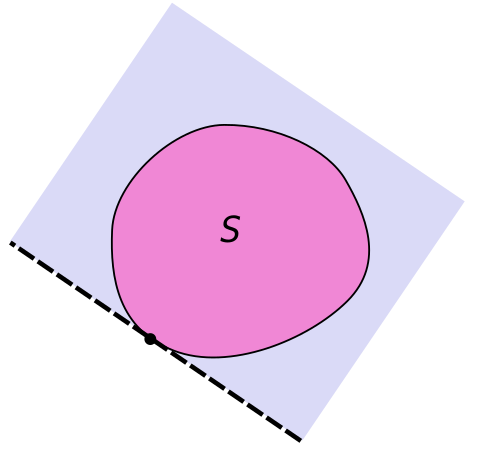
\includegraphics[width=.3\textwidth]{images/supporting-hyperplane.png}
     \caption{Supporting hyperplane for a set $S$.}
     \label{fig:supporting-hyperplane}
 \end{figure}
 
 \cor[supporting-hyperplane]{Supporting hyperplane theorem}{
     Let $K\subset \bbR^d$ be a convex set and $x\in\partial K$. Then, there exists a supporting hyperplane of $K$ containing $x_0$.
     That is, there exists $v\in\bbR^d$ and $\lambda\in\bbR$ such that $K\subset H_{v,\lambda}$ and $x_0\in \partial H_{v,\lambda}$.
 }
 
 When $K$ is a convex polygon, it is natural to expect it to be determined by its vertices. In order to formalize this intuition we need the following.
 
 \dfn{}{
     Let $K\subset\bbR^d$ be a convex set. A point $x\in K$ is an extremum of $K$ if for any $y,z\in K$ and $t\in (0,1)$ we have that
     \begin{equation}
         x = t y +(1-t) z \implies x=y=z.
     \end{equation}
     The set of exterma of $K$ is denoted by $\operatorname{extr}(K)$.
 }
 
 In particular, for a convex polygon $\operatorname{extr}(K)$ is the set of its vertices.
 
 \prop{}{
     Let $K\subset\bbR^d$ be a convex set that is compact. Then,
     \begin{equation}
         \operatorname{conv}(K)= \operatorname{conv}\left(\operatorname{extr}(K)\right).
     \end{equation}
 }
 
 \section{Cones}
 
 \dfn{}{
     A set $K\subset \bbR^d$ is a cone if
     \begin{equation}
         tx \in K \qquad \forall x\in K, \, t\ge 0.
     \end{equation}
 }
 
 Observe that every cone contains the origin.
 
 \ex{Cones}{
     \begin{itemize}
         \item The second order cone $$C = \{ x=(x',x_n)\in \bbR^{d}\times \bbR \mid \|x'\|_2 \le x_n\}.$$
         \item Positive orthant $\bbR_+^d = \{ x\in\bbR^d \mid x_i\ge 0, \quad \forall i\in \llbracket 1,d\rrbracket \}$.
         \item The set of positive semidefinite matrices $\operatorname{Sym}_+(\bbR^d)$.
     \end{itemize}
 }
 
 \dfn{}{
     The conic hull $\operatorname{cone}(\Omega)$ of a set $\Omega\subset \bbR^d$ is the smallest cone containing $\Omega$. Namely,
     \begin{equation}
         \operatorname{cone}(\Omega) = \left\{ \sum_{i=1}^n t_i x_i \mid t_i\ge 0\text{ and } x_i\in \Omega  \text{ for any } i \in \llbracket 1,n\rrbracket   \right\}.
     \end{equation}
 }
 
 \dfn[dual-cone]{}{
     The dual cone $K^*$ of a cone $K\subset\bbR^d$ is the set
     \begin{equation}
         K^* := \left\{ y\in\bbR^d \mid \langle x,y \rangle \ge 0 \quad \forall x\in K \right\}.
     \end{equation}
 }
 
 \begin{figure}[t]
     \centering
     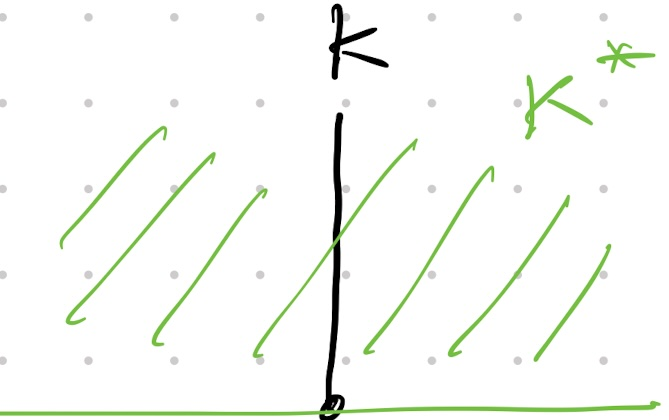
\includegraphics[width=.3\textwidth]{images/polar-cone-1}
     \hspace{.1\textwidth}
     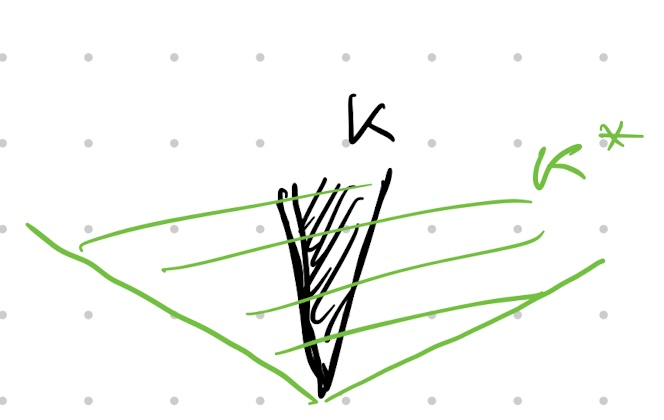
\includegraphics[width=.3\textwidth]{images/polar-cone-2}
     \caption{Two examples of polar cone.}
 \end{figure}
 
 We 	have the following properties for the polar cone.
 
 \prop{}{
     The dual cone $K^*$ is a closed, convex cone. If, moreover, the cone $K$ is closed and convex, then $K^{**}=K$.
 }
 
 \begin{proof}
     The fact that $K^*$ is closed follows immediately by continuity of $y\mapsto \langle x,y\rangle$ for any $x\in K$.
     To show that $K^*$ is convex, let $y,z\in K^*$, $x\in K$, and compute
     \begin{equation}
         \langle ty + (1-t)z, x\rangle = t \langle y, x\rangle +(1-t) \langle z,x\rangle \ge 0 \qquad \forall t\in [0,1].
     \end{equation}
 
     Consider now $x\in K$. By definition of $K^*$ we have that $\langle x,y\rangle\ge 0$ for all $y\in K^*$, which implies that $K\subset K^{**}$.
 
     In order to show the opposite inclusion, we will show that $x\notin K$ implies that $x\notin K^**$. Let $x\notin K$ and observe that then $\{x\}$ is a convex set whose interior is disjoint from $K$. By the Separation Theorem~\ref{th:separation}, there exists $v\in \bbR^d$ and $\lambda\in\bbR$ such that
     \begin{equation}
         \langle y,v \rangle\ge  \lambda\qquad \forall y\in K
         \qquad\text{and}\qquad
         \langle x,v \rangle < \lambda.
     \end{equation}
     Since $0\in K$, for the above to be true it has to hold $\lambda \le 0$, and hence it holds
     \begin{equation}
         \langle y,v \rangle\ge  0\qquad \forall y\in K
         \qquad\text{and}\qquad
         \langle x,v \rangle < 0.
     \end{equation}
     In particular, the first part of the above yields $v\in K^*$. Hence, the second part of the above yields $x\notin K^**$, as desired.
 \end{proof}
 
 \begin{remark}
     The convexity assumption in the above is essential, a counterexample is easily constructed by considering $K$ to be the union of two half-lines.
     In general, $K^{**} = \overline{\operatorname{conv}(K)^{**}}$.
 \end{remark}
 
 \section{Convex functions}
 
 We will work with extended functions $F:\bbR^d\to \bbR\cup\{+\infty\}$. The domain of an extended function is
 \begin{equation}
     \operatorname{dom}(F) = \{x\in \bbR^d\mid F(x)<+\infty\}.
 \end{equation}
 An extended function such that $\operatorname{dom}(F)\neq \varnothing$ is called \emph{proper}.
 
 Given a standard function $F:\Omega\to \bbR$, we can identify it with the extended function $\bar F:\bbR^d\to \bbR\cup\{+\infty\}$ defined by
 \begin{equation}
     \bar F(x) =
     \begin{cases}
         F(x)    & \text{if }x\in \Omega,                 \\
         +\infty & \text{if }x\in \bbR^d\setminus \Omega.
     \end{cases}
 \end{equation}
 
 \dfn{Convex functions}{
     Let $F:\bbR^d\to\bbR\cup\{+\infty\}$ be an extended function. Then,
     \begin{itemize}
         \item $F$ is convex if
               \begin{equation}
                   F(tx + (1-t)y) \le t F(x) + (1-t)F(y) \qquad \forall x,y\in \bbR^d,\, t\in [0,1].
               \end{equation}
         \item $F$ is strictly convex if
               \begin{equation}
                   F(tx + (1-t)y) < t F(x) + (1-t)F(y) \qquad \forall x,y\in \bbR^d,\, x\neq y, \, t\in [0,1].
               \end{equation}
         \item $F$ is strongly convex if there exists $\gamma>0$ such that
               \begin{equation}
                   F(tx + (1-t)y) \le t F(x) + (1-t)F(y) - \frac{\gamma}{2}t(t-1)\|x-y\|_2^2 \qquad \forall x,y\in \bbR^d,\, t\in [0,1].
               \end{equation}
     \end{itemize}
 
     We say that $F$ is \emph{concave} if $-F$ is convex.
 }
 
 Observe that it holds
 \begin{equation}
     \text{convex} \impliedby \text{strongly convex} \impliedby \text{strictly convex}
 \end{equation}
 
 We say that a standard function $F:K\to \bbR$ is convex, strictly convex, strongly convex, or concave, if the same is true for its extension $\bar F$. Observe that this requires $K$ to be convex.
 
 \ex{}{
     \begin{itemize}
         \item 	The prototypical convex function, used in the definition of strongly convex, is the quadratic function
               \begin{equation}
                   F(x) = \frac{\|x\|_2^2}{2} = \frac{1}{2}\sum_{i=1}^d |x_i|^2.
               \end{equation}
         \item More generally, every norm is convex.
         \item The norm $\ell_p$ is strictly convex if and only if $p\in (1,+\infty)$.
         \item $F(x) = x^\top A x$ is convex if $A$ is positive semidefinite (i.e.,  $A\in \operatorname{Sym}_{\ge 0}(\bbR^d)$), and strongly convex if $A$ is positive definite.
     \end{itemize}
 }
 
 \prop[epigraph]{}{
     A function $F:K\to\bbR$ is convex if and only if its epigraph $\operatorname{epi}(F)\subset \bbR^{d+1}$ is convex. Here, we let
     \begin{equation}
         \operatorname{epi}(F) = \{ (x,r) \mid r\ge F(x) \}.
     \end{equation}
 }
 
 \begin{figure}
     \begin{minipage}{.48\textwidth}
         \centering
         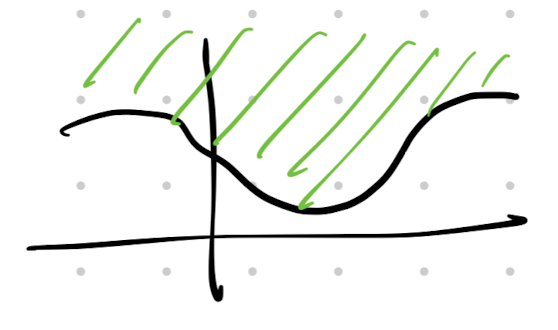
\includegraphics[width=.6\textwidth]{images/epigraph.png}
         \caption{Epigraph of a function.}
     \end{minipage}
     \begin{minipage}{.48\textwidth}
         \centering
         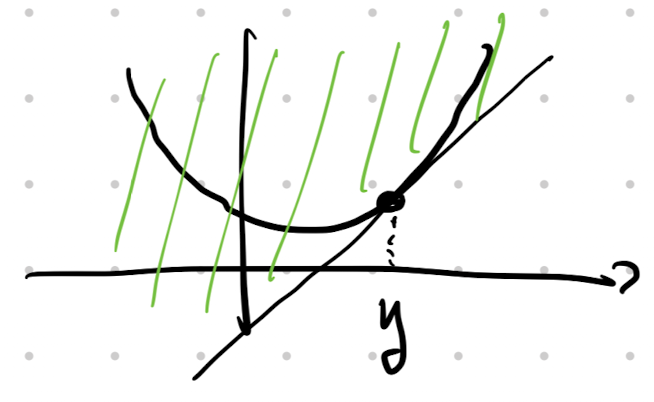
\includegraphics[width=.6\textwidth]{images/convexity-diff.png}
         \caption{Graphical representation of Proposition~\ref{prop:convexity-diff}.}
     \end{minipage}
 \end{figure}
 
 \begin{proof}
     Assume $F$ is convex and let $(x,r),(y,s)\in\operatorname{epi}(F)$.
     In particular, $r\ge F(x)$ and $s\ge F(y)$.
     Let $t\in [0,1]$ and observe that
     \begin{equation}
         t r +(1-t)s \ge t F(x)+(1-t)F(y) \ge  F(tx+(1-t)y).
     \end{equation}
     Hence, $t(x,r) + (1-t)(y,s)\in\operatorname{epi}(F)$. A similar reasoning proves the opposite implication.
 \end{proof}
 
 \prop[convexity-diff]{Differential characterisations of convexity}{
     Let $F:\bbR^d \to \bbR$ be an everywhere differentiable function. Then,
     \begin{itemize}
         \item $F$ is convex if and only if
               \begin{equation}
                   \label{eq:supporting-hyper-fct}
                   F(y) \ge F(x) + \langle \nabla F(x), y-x \rangle, \qquad \forall x,y\in \bbR^d.
               \end{equation}
         \item $F$ is strongly convex with parameter $\gamma>0$ if and only if
               \begin{equation}
                   F(y) \ge F(x) + \langle \nabla F(x), y-x \rangle + \frac{\gamma}{2}\|x-y\|^2_2, \qquad \forall x,y\in \bbR^d.
               \end{equation}
         \item If $F$ is everywhere twice differentiable, then it is convex if and only if
               \begin{equation}
                   \operatorname{Hess} F(x) \ge 0 \qquad \forall x\in\bbR^d,
               \end{equation}
               and strongly convex if and only if there exists $\gamma>0$ such that
               \begin{equation}
                   \operatorname{Hess} F(x) \ge \frac{\gamma}2 \qquad \forall x\in\bbR^d.
               \end{equation}
               Here, we denoted by $\operatorname{Hess}F(x)$ the Hessian of $F$ at $x$.
     \end{itemize}
 }
 
 \prop[convex-cont]{}{
     Let $F:K\to \bbR$ be convex. Then, $F$ is continuous on the interior of $K$.
 }
 
 \begin{proof}
     Let $x_0\in \operatorname{int}(K)$ and consider $r>0$ such that $B(x_0,r)\subset K$. Without loss of generality, we assume $x_0=0$ (otherwise, replace the function $F$ by its translation $G(x) = F(x)-F(x_0)$).
 
     Convexity will allow to bound the difference $F(y)-F(0)$ with the values of $F$ on the sphere $\partial B(0,r)$.
     However, without continuity, the function $F$ need not be bounded on the compact set $\partial B(0,r)$, and hence we need some additional care.
 
     Pick $d+1$ linearly independent points $v_0,\ldots v_{d+1}\in \partial B(0,r)$, and consider the corresponding symplex
     \begin{equation}
         \Delta = \operatorname{conv}\left(\{v_0,\ldots,v_{d+1}\}  \right)
         = \left\{  \sum_{i=1}^{d+1} t_i v_i \mid t_i\ge 0,\, \sum_i t_i=1 \right\}\subset B(0,r).
     \end{equation}
     Then, letting $M = \max_{i\in \llbracket1,d+1 \rrbracket} F(v_i)$, the fact that $F$ is convex yields that for any $x=\sum_{i=1}^{d+1} t_i v_i\in \Delta$ it holds
     \begin{equation}
         \label{eq:bdd}
         F(x) \le \sum_{i=1}^{d+1} t_i F(v_i) \le M.
     \end{equation}
     In particular, we can fix a radius $r'<r$ such that  $B(0,r')\subset \Delta$ where $F$ is bounded.
 
     We now proceed to bound the difference $F(x)-F(0)$.
     Let $x\in U\subset B(0,r')$ and set $t = \|x\|/r'$. In particular, $t\in [0,1]$ and the ray $\{sx\mid s\ge 0$ meets the sphere $\partial B(x_0,r')$ at the point
     \begin{equation}
         y= \frac{r'}{\|x\|}(x).
     \end{equation}
     In particular, $x=(1-t)0 + ty$. By convexity and \eqref{eq:bdd}, we have
     \begin{equation}
         \label{eq:upper}
         F(x) \le (1-t) F(0) + t F(y) \le. (1-t)F(0)+ t M
         \implies
         F(x)-F(0) \le t(M-F(0)).
     \end{equation}
 
     To derive a bound from below, we proceed similarly, considering
     \begin{equation}
         z = \frac{r'}{\|x\|-r'}x.
     \end{equation}
     Indeed, we then have $0 = (1-t)x + t x$, where $t=\|x\|/r'$ as above. Then, convexity and the fact that $z\in B(0,r')$ yield
     \begin{equation}
         \label{eq:lower}
         F(0)\le (1-t)F(x) +tM \implies F(x)-F(0)\ge -\frac{t}{1-t}(M-F(0)).
     \end{equation}
 
     Combining \eqref{eq:upper} and \eqref{eq:lower}, we obtain
     \begin{equation}
         - \frac{t}{1-t}(M-F(0)) \le F(x)-F(0) \le t(M-F(0)), \qquad t=\frac{\|x\|}{r'}
     \end{equation}
     Since $x$ was arbitrary in $B(0,r')$ we can take the limit as $x\to 0$, which implies $t\to 0$ and thus that
     \begin{equation}
         \lim_{x\to 0}|F(x)-F(0)|=0,
     \end{equation}
     concluding the proof.
 \end{proof}
 
 The following result is at the core of the relation between optimisation and convexity.
 
 \thm[min-convex]{}{
     Let $F:\bbR^d\to \bbR\cup\{+\infty\}$ be a convex extended function. Then,
     \begin{itemize}
         \item Any local minimum of $F$ is global.
         \item The set of minima of $F$ is convex.
         \item If $F$ is strictly convex and admits a minimum, this minimum is unique.
         \item If $F$ is real-valued and strongly convex, then it has a unique minimum.
     \end{itemize}
 }
 
 \begin{proof}
     Assume that $x^\star$ is a local minimum, i.e., there exists $r>0$ such that $F(x^\star)\le F(x)$ for any $x\in B(0,r)$.
     Let $y\in \bbR^d$ and consider a point on the ray starting at $x^\star$ and passing through $y$:
     \begin{equation}
         z = x^\star + s (y-x^\star) =   (1-s)x^\star + s y\qquad s\ge 0.
     \end{equation}
     Taking $s < \min\{1, r'/\|x^\star - y\|\}$ we have that $z\in B(0,r)$. Hence, by local minimality of $x^\star$ and convexity of $F$ we have
     \begin{equation}
         F(x^\star) \le F(z) \le (1-s)F(x^\star) + s F(y) \implies F(x^\star) \le F(y).
     \end{equation}
     This concludes the proof of the first point.
 
     Assume now that $x_1,x_2$ are minima for $F$. This clearly implies that $F(x_1)=F(x_2) =: m$, and thus, by convexity of $F$, for any $t\in [0,1]$ we have
     \begin{equation}
         m \le F(t x_1 + (1-t)x_2) \le t F(x_1) +(1-t) F(x_2) = m \implies F(t x_1 + (1-t)x_2).
     \end{equation}
     This implies that $t x_1 + (1-t)x_2$ is a minimum for any $t\in [0,1]$, thus proving the second point.
 
     The same argument as above in the case of a strictly convex function yields to
     \begin{equation}
         m \le F(tx_1+(1-t)x_2) < m \qquad \text{ if } x_1\neq x_2.
     \end{equation}
     This implies immediately that the minimum is unique.
 
     Assume, finally, that $F$ is strongly convex. Since it is strictly convex, we just need to prove the existence of a minimum.
     By Proposition~\ref{prop:convex-cont} we have that $F$ is continuos, and thus it suffices to prove its coercivity: $F(x)\to +\infty$ if $\|x\|\to +\infty$.
     We provide a proof of this fact in the case where $F$ is differentiable (the general case can be obtained similarly using Proposition~\ref{prop:subdifferential}, proven later on). In this case, by Proposition~\ref{prop:convexity-diff} we have that
     \begin{equation}
         F(y) \ge F(0)+\langle \nabla F(0),y\rangle +\frac\gamma2\|y\|_2^2 \qquad \forall y\in \bbR^d.
     \end{equation}
     Since $\langle \nabla F(0),y\rangle \le \|y\|_2$, the quadratic term on the right-hand side of the above equation, implies that the limit as $\|y\|_2\to +\infty$ is $+\infty$.
 \end{proof}
 
 \begin{remark}
     Strict convexity is not enough to ensure the existence of a minimum. Consider, for example, $F(x) = e^x$.
 \end{remark}
 
 \section{Convex conjugate and sub-differential}
 \label{sec:conjugate-fct}
 
 \dfn{}{
     The convex conjugate (of Fenchel dual)  of an extended function $F:\bbR^d\to \bbR\cup\{+\infty\}$ is the function $F^*:\bbR^d\to \bbR\cup\{+\infty\}$ defined by
     \begin{equation}
         F^*(y) = \sup_{x\in\bbR^d}\left[\langle x,y\rangle-F(x)\right].
     \end{equation}
 }
 
 Recall the following.
 
 \dfn{}{A function $F:\bbR^d\to \bbR$ is \emph{lower semicontinuous} (l.s.c.) if
     \begin{equation}
         \liminf_{x\to x_0} F(x) \ge F(x_0), \qquad \forall x_0\in\bbR^d.
     \end{equation}
     Equivalently, $F$ is l.s.c.~if its epigraph is closed.
 }
 
 \ex{}{
     \begin{itemize}
         \item Every continuous function is lower semicontinuous.
         \item For any set $\Omega\subset \bbR^d$, the $0-\infty$ characteristic function
               \begin{equation}
                   \label{eq:0-infty-char}
                   \chi_K=\begin{cases}
                       0       & \text{if } x\in\Omega, \\
                       +\infty & \text{otherwise},
                   \end{cases}
               \end{equation}
               is lower semicontinuous, but not continuous.
     \end{itemize}
 }
 
 
 \prop[convex-conj-prop]{}{
     Let $F:\bbR^d\to \bbR\cup\{+\infty\}$. Then,
     \begin{enumerate}
         \item The convex conjugate $F^*$ is a lower semicontinuous convex function.
         \item We have the Fenchel (or Young, or Fenchel-Young) inequality
               \begin{equation}
                   \langle x,y\rangle \le F(x)+F^*(y)
               \end{equation}
     \end{enumerate}
 }
 
 \begin{proof}
     For any $y_1,y_2\in\bbR^d$ and $t\in[0,1]$ we have
     \begin{equation}
         \langle x, ty_1+(1-t)y_2 \rangle-F(x) =
         t \left(\langle x, y_1\rangle-F(x)\right) + (1-t) \left(\langle x, y_2\rangle-F(x)\right).
     \end{equation}
     Taking the supremum for $x\in\bbR^d$ of the above, and recalling that $\sup(g(x)+h(x))\le \sup g(x)+\sup h(x)$ proves convexity of $F^*$.
 
     Lower semicontinuity of $F^*$ follows since it is the supremum for $x\in\bbR^d$ of $g_x(y):=\langle x,y\rangle -F(x)$, which is affine and in particular lower semicontinuous. Indeed, the supremum of a family of l.s.c.~functions is l.s.c..
 
     The second point (Fenchel inequality) is a direct consequence of the definition of $F^*$.
 \end{proof}
 
 
 
 
 \ex{}{
     \begin{itemize}
         \item Let $F(x)=\frac12 \|x\|_2^2$. Then, $F^*(y)=\frac12\|y\|_2^2=F(y)$. This is the only function with this property.
         \item Let $F=\chi_K$ be the $0-\infty$ characteristic function of a convex set $K\subset\bbR^d$ defined in \eqref{eq:0-infty-char}. Then,
               \begin{equation}
                   F^*(y)=\sup_{x\in K} \langle x,y\rangle.
               \end{equation}
     \end{itemize}
 }
 
 \dfn{}{
     The \emph{subdifferential} of a convex extended function $F:\bbR^d\to \bbR\cup\{+\infty\}$ at $x\in\bbR^d$ is the set
     \begin{equation}
         \partial F(x) = \left\{ v\in\bbR^d \mid F(y) \ge F(x)+\langle v,y-x \rangle, \qquad \forall y\in\bbR^d \right\}.
     \end{equation}
     A vector $v\in \partial F(x)$ is called a \emph{subgradient} for $F$ at $x$.
 }
 
 \begin{figure}
     \centering
     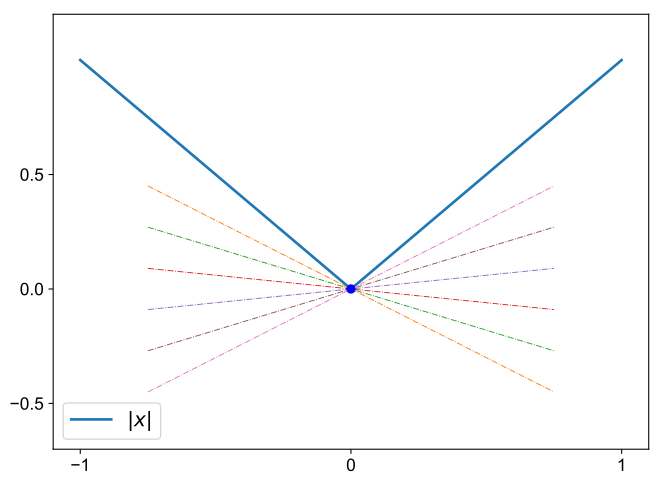
\includegraphics[width=.4\textwidth]{images/abs-subgrad.png}
     \caption{Visualization of the subgradients of $F(x)=|x|$ at $x=0$. Image from \href{https://tlienart.github.io/posts/2018/09/23-convex-optimisation-1/}{this website}.}
     \label{fig:subgrad-abs}
 \end{figure}
 
 \ex{}{
     Consider $F(x)=|x|$. Then,
     \begin{equation}
         \partial F(x) =
         \begin{cases}
             \{ \operatorname{sgn}(x) \} & \text{if }x\neq 0, \\
             [-1,1]                      & \text{if } x=0.
         \end{cases}
     \end{equation}
     Here, $\operatorname{sgn}(x) = x/|x|$ is the sign function.
     See Figure~\ref{fig:subgrad-abs}.
 }
 
 \thm[suff-cond-minimum]{}{
     Let $F:\bbR^d\to \bbR\cup\{+\infty\}$ be a convex function. Then, $x\in\bbR^d$ is a minimum for $F$ if and only if $0\in \partial F(x)$
 }
 
 \begin{proof}
     The fact that $x$ is a minimum means that $F(x)\le F(y)$ for any $y\in\bbR^d$, which is the definition of $0\in\partial F(x)$.
 \end{proof}
 
 We have the following.
 
 \prop[subdifferential]{}{
     Let $F:\bbR^d\to \bbR\cup \{+\infty\}$ be a convex function. Then,
     \begin{itemize}
         \item For any $x\in \bbR^d$ the subdifferential $\partial F(x)$ is non-empty.
         \item It holds that
               \begin{equation}
                   \partial F(x) = \left\{ v\in \bbR^d\mid F^*(v) + F(x) = \langle x,v\rangle  \right\}.
               \end{equation}
         \item If $F$ is differentiable at $x\in\bbR^d$, then $\partial F(x)=\{\nabla F(x)\}$.
     \end{itemize}
 }
 
 \begin{proof}
     The first part of the theorem is a consequence of the Supporting Hyperplane Theorem (see Corollary~\ref{th:supporting-hyperplane}) and Proposition~\ref{prop:epigraph}. Indeed, the latter implies that the epigraph $\operatorname{epi}(F)$ is convex and hence, by the former, any of its boundary point admits a supporting hyperplane. Using the fact that $\partial\operatorname{epi}(F)=\{(x,F(x))\mid x\in\bbR^d\}$ allows to conclude.
 
     To prove the second statement, observe that $v\in\partial F(x)$ is equivalent to
     \begin{equation}
         \langle y,v\rangle - F(y) \le \langle x,v\rangle-F(x), \qquad \forall y\in\bbR^d.
     \end{equation}
     Taking the sup for $y\in\bbR^d$ yields that $F^*(v)\le \langle x,v\rangle -F(x)$. The opposite inequality follows from Fenchel inequality (see Proposition~\ref{prop:convex-conj-prop}).
 
     Concerning the proof of the last statement, the fact that $\nabla F(x)\in \partial F(x)$ follows from the characterisation of convexity for differentiable functions given in Proposition~\ref{prop:convexity-diff}.
     To prove the opposite implication, let $v\in \partial F(x)$ and observe that by definition of subgradient the directional derivative $\partial_h F(x)$ of $f$ in the direction $h\in\bbR^d$ at $x$ satisfies
     \begin{equation}
         \partial_h F(x) = \lim_{t\to 0} \frac{F(x+th)-F(x)}{t} \ge \langle v, h\rangle.
     \end{equation}
     Since we know that $\partial_hF (x)=\langle \nabla F(x),h\rangle$, we have that
     \begin{equation}
         \langle \nabla F(x) - v,h\rangle \ge 0, \qquad \forall h\in\bbR^d.
     \end{equation}
     But this implies that $\nabla F(x)=v$, concluding the proof.
 \end{proof}
 
 
 
 Thanks to the previous result, we are in a position to prove the following property of the convex biconjugate.
 
 \thm[fenchel-moreau]{Fenchel-Moreau Theorem}{
     The biconjugate $F^{**}$ is the largest convex lower semicontinuous function satisfying $F^{**}(x)\le F(x)$ for any $x\in \bbR^d$. In particular, $F^{**}=F$ if $F$ is convex and proper.
 }
 
 \begin{proof}
     % We start by proving that for any extended function $F$ it holds
     % \begin{equation}
     % 	F^{**}(x)\le F(x), \qquad \forall x\in\bbR^d.
     % \end{equation}	
     % Indeed, w
     We have that $-F^*(y)=\inf_{x\in\bbR^d} \left(F(x)-\langle x,y\rangle\right)$, which implies that for any $y,z\in\bbR^d$ it holds
     \begin{equation}
         \langle z,y\rangle - F^*(y) \le \langle z-x,y\rangle +F(x), \qquad \forall x\in\bbR^d.
     \end{equation}
     In particular, considering $z=x$ we have
     \begin{equation}
         F^{**}(x) = \sup_{y\in\bbR^d} \left(\langle x,y\rangle - F^*(y)\right) \le F(x),
     \end{equation}
     proving the first part of the statement.
 
     Since $F^{**}$ is convex and l.s.c.~by Proposition~\ref{prop:convex-conj-prop}, in order to complete the proof it suffices to show that if $F$ is convex, then
     \begin{equation}
         F^{**}(x)\ge F(x),\qquad \forall x\in\bbR^d.
     \end{equation}
     Let $v\in \partial F(x)$, which exists thanks to Proposition~\ref{prop:subdifferential}. For such a $v$, using the characterisation of the subdifferential in Proposition~\ref{prop:subdifferential}, we have
     \begin{equation}
         F^*(v)=\langle x,v\rangle - F(x),
     \end{equation}
     so that $F^{**}(z)\ge \langle v,z-x\rangle+F(x)$ for any $z\in \bbR^d$. Picking $z=x$ allows to conclude.
 \end{proof}
 
 
 
 \prop{subdiff-conj}{
     Let $F:\bbR^d\to \bbR\cup\{+\infty\}$ be a convex function and $x,y\in \bbR^d$. Then, the following are equivalent:
     \begin{enumerate}
         \item[i.] $y\in \partial F(x)$.
         \item[ii.] $F(x)+F^*(y) = \langle  x,y\rangle$.
     \end{enumerate}
     If, additionally, $F$ is l.s.c.~, then the above are also equivalent to
     \begin{enumerate}
         \item[iii.] $x\in \partial F^*(y)$.
     \end{enumerate}
 }
 
 \begin{proof}
     To show that \emph{i} is equivalent to \emph{ii}, we just need to show that $y\in \partial F(x)$ is equivalent to
     \begin{equation}
         \label{eq:opp-fenchel-ineq}
         F(x)+F^*(y) \le \langle  x,y\rangle.
     \end{equation}
     Indeed, the opposite inequality is always true due to Fenchel's inequality (see Proposition~\ref{prop:convex-conj-prop}).
 
     Observe that the fact that $y\in\partial F(x)$ means that
     \begin{equation}
         \langle x,y\rangle F(x)
         \ge \langle z,y\rangle F(z), \qquad \forall z\in \bbR^d.
     \end{equation}
     That is, the function $z\mapsto \langle z,y\rangle F(z)$ attains its maximum at $z=x$. But, by definition of $F^*$, this is equivalent to \eqref{eq:opp-fenchel-ineq}, thus proving that \emph{i} is equivalent to \emph{ii}.
 
     To complete the proof, observe that by Theorem~\ref{th:fenchel-moreau} the lower semicontinuity of $F$ yield that $F^{**}=F$, so that \emph{ii} is equivalent to $F^{**}(x)+F^*(y)=\langle x,y\rangle$. Using the fact that \emph{i}$\iff$\emph{ii} with $F$ replaced by $F^*$ completes the proof.
 \end{proof}
 
 \section{Proximal operator}
 \label{sec:proximal}
 
 \dfn{Proximal operator}{
     Let $F:\bbR^d\to \bbR\cup \{+\infty\}$ be a convex function. The proximal operator associated with $F$ is
     \begin{equation}
         P_F(y) = \arg\min_{x\in\bbR^d}\left\{ F(x) + \frac12 \|x-y\|^2_2 \right\}.
     \end{equation}
 }
 
 The above definition makes sense, since $x\mapsto F(x) + \frac12 \|x-y\|^2$ is a strongly convex function and hence has a unique minimum by Theorem~\ref{th:min-convex}.
 
 \ex{Proximal operator of a convex set}{
     Let $F=\chi_K$ be the $0$-$\infty$ characteristic function of a convex set. Then, $P_K = P_{\chi_K}$ is the orthogonal projection onto $K$, that is
     \begin{equation}
         P_F(y) = \arg\min_{x\in K}\left\{ \|x-y\|^2 \right\}.
     \end{equation}
 }
 
 \ex[soft-thresholding]{Soft-thresholding}{
     Let $F(x) = |x|$ for $x\in\bbR$. Then, for any $\lambda>0$,
     \begin{equation}
         \label{eq:soft-thresholding}
         P_{\lambda F}(y):=S_\lambda(y) =
         \begin{cases}
             y+\lambda & \text{if } y \le -\lambda, \\
             0         & \text{ if } |y|<\lambda ,  \\
             y-\lambda & \text{if } y \ge\lambda,   \\
         \end{cases}
     \end{equation}
     This function is known as soft-thresholding. See Figure~\ref{fig:soft-thresholding}.
 }
 
 \begin{figure}
     \centering
     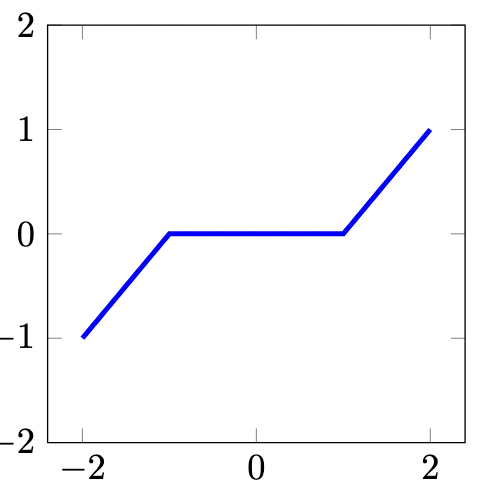
\includegraphics[width=.3\textwidth]{images/soft-thresholding.png}
     \caption{Soft-thresholding function.}
     \label{fig:soft-thresholding}
 \end{figure}
 
 
 The following proposition shows the relation between the proximal operator and the subdifferential, and justifies the notation
 \begin{equation}
     P_F = (\operatorname{Id} + \partial F)^{-1}.
 \end{equation}
 
 \prop[prox-subdiff]{}{
     Let $F:\bbR^d\to \bbR\cup \{+\infty\}$ be a convex function, then, for any $x,y\in\bbR^d$,
     \begin{equation}
         P_F(y) = x
         \iff
         y \in x + \partial F(x).
     \end{equation}
 }
 
 \begin{proof}
     By Theorem~\ref{th:suff-cond-minimum}, we have that $x=P_F(y)$ if and only if
     \begin{equation}
         0 \in \partial\left[ \frac12 \|\cdot-y\|_2^2 + F(\cdot)\right](x) = x - y +\partial F(x).
     \end{equation}
     Here, we used differentiability of $x\mapsto \|x-y\|_2^2$. This completes the proof.
 \end{proof}
 
 An important property of the proximal operator is the following.
 
 \prop[prox-non-exp]{Non-expansiveness of the proximal operator}{
     Let $F:\bbR^d\to \bbR\cup \{+\infty\}$ be a convex function, then the proximal operator is non-expansive. Namely,
     \begin{equation}
         \|P_F(y_1)-P_F(y_2)\|_2^2 \le \|y_1-y_2\|_2^2, \qquad \forall y_1,y_2\in\bbR^d.
     \end{equation}
 }
 
 \begin{proof}
     Let $x_i = P_F(y_i)$. Then, by Proposition~\ref{prop:prox-subdiff} we have $y_i \in x_i+\partial F(x_i)$. In particular, $y_i - x_i \in \partial F(x_i)$ and thus, by definition of subdifferential,
     \begin{gather}
         F(x_2) \ge F(x_1) + \langle y_1-x_1,x_2-x_1 \rangle
         \qquad\text{and}\qquad
         F(x_1) \ge F(x_2) + \langle y_2-x_2,x_1-x_2 \rangle .
     \end{gather}
     Summing up, we get $0\ge \langle x_1-y_1+y_2-x_1,x_1-x_2 \rangle$, which yields
     \begin{equation}
         \|x_1-x_2\|_2^2 \le \langle y_1-y_2,x_1-x_2\rangle.
     \end{equation}
     Applying Cauchy-Schwarz inequality allows to conclude.
 \end{proof}
 
 The following relates the proximal operator of $F$ and of its complex conjugate $F^*$, defined in Section~\ref{sec:conjugate-fct}.
 
 \thm[moreau-ident]{Moreau's Identity}{
     Let $F:\bbR^d\to \bbR\cup\{+\infty\}$ be a lower semicontinuous convex function. Then,
     \begin{equation}
         P_F(y) + P_{F^*}(y) = y, \qquad \forall y\in \bbR^d.
     \end{equation}
 }
 
 \begin{proof}
     Let $x = P_F(y)$ and set $z=y-x$. By Proposition~\ref{prop:prox-subdiff} we thus have $z\in \partial F(x)$. Since $F$ is lower semicontinuous, we have from Proposition~\ref{prop:subdiff-conj} that $x\in \partial F^*(z)$ Since this is equivalent to $y\in z + \partial F^*(z)$, Proposition~\ref{prop:prox-subdiff} implies that $z = P_{F^*}(y)$. Thus,
     \begin{equation}
         P_F(y) + P_{F^*}(y) = x + z = y.
     \end{equation}
 \end{proof}
 
 
 \chapter{Optimization problems}
 
 \section{Convex optimization problems}
 \label{chp:optimization-problems}
 
 \dfn{}{
     An optimization problem is a minimization problem of the form
     \begin{equation}
         \tag{OP}
         \label{eq:op}
         \min_{x\in \bbR^d} F_0(x)
         \qquad\text{subject to}\qquad
         Ax=y
         \qquad \text{and}\qquad
         F_j(x)\le 0, \qquad j\in\llbracket 1, M\rrbracket.
     \end{equation}
     Here,
     \begin{enumerate}
         \item $F_0:\bbR^d\to \bbR\cup\{+\infty\}$ is the \emph{objective function};
         \item $F_1,\ldots, F_M:\bbR^d\to \bbR\cup\{+\infty\}$ are the \emph{constraing functions};
         \item $A\in \bbR^{m\times n}$ and $y\in \bbR^m$ provide the \emph{equality constraints};
     \end{enumerate}
 
     The optimization problem is \emph{convex} (resp.~\emph{linear}) if $F_0,\ldots, F_M$ are convex (resp.~linear) functions.
 }
 
 \dfn{}{
     Consider an optimization problem \eqref{eq:op}. Then,
     \begin{itemize}
         \item The set $\feas\subset\bbR^d$ of points $x\in\bbR^d$ satisfying the constraints is the set of \emph{feasible points}. That is,
               \begin{equation}
                   \feas = \left\{ x\in \bbR^d \mid Ax = y, \qquad F_j(x)\le 0 \qquad \forall j\in \llbracket 1,M\rrbracket \right\}.
               \end{equation}
               In particular, $\feas$ is convex if \eqref{eq:op} is convex.
         \item Problem \eqref{eq:op} is \emph{feasible} if it admits at least a feasible point (i.e., $\feas\neq \varnothing$).
         \item The \emph{optimal value} is $p^\star = \min_{x\in\feas} F(x_0)$.
         \item A \emph{minimizer} is a feasible point $x^\star$ such that $F_0(x^\star)\le F_0(x)$ for all feasible $x\in \feas$. That is, $F_0(x^\star)=p^\star$.
     \end{itemize}
 }
 
 Observe that the constrained optimization problem \eqref{eq:op} is equivalent to the uncostrained optimization problem
 \begin{equation}
     \min_{x\in \bbR^d} F_0(x) + \chi_{\feas},
 \end{equation}
 where $\chi_{\feas}$ is the $0-\infty$ characteristic function defined in \eqref{eq:0-infty-char}.
 
 Let us introduce the notation
 \begin{equation}
     \bbR^M=\{\nu\in \bbR^M\mid \nu_j\ge 0\quad \forall j\in \llbracket 1,M\rrbracket\}.
 \end{equation}
 
 \dfn{Lagrange and Lagrange dual functions}{
     The \emph{Lagrange function} of the optimization problem \eqref{eq:op} is the function $F:\bbR^d \times \bbR^m \times \bbR^M_+\to \bbR\cup\{+\infty\}$ defined by
     \begin{equation}
         L(x,\xi,\nu) = F_0(x) + \langle \xi, Ax-y\rangle +\sum_{j=1}^m \nu_j F_j(x).
     \end{equation}
 
     The \emph{Lagrange dual function} is the function $H:\bbR^m\times \bbR^M_+ \to \bbR\cup\{-\infty\}\cup\{+\infty\}$, defined by
     \begin{equation}
         H(\xi,\nu) = \inf_{x\in \bbR^d} L(x,\xi,\nu).
     \end{equation}
 }
 
 \prop[weak-duality]{}{
     The dual function is always concave. Moreover, if $x^\star$ is a minimizer of \eqref{eq:op}, we have
     \begin{equation}
         H(\xi,\nu) \le F(x^\star), \qquad \forall \xi\in \bbR^m,\, \nu\in \bbR^M_+.
     \end{equation}
 }
 
 \begin{proof}
     Observe that $-H$ is the supremum w.r.t.~$x\in \bbR^d$ of the functions $g_x(\xi,\nu) = -L(x,\xi,\nu)$. The function $g_x$ is affine, and thus convex. Hence, $-H$ is the pointwise supremum of the family $\{g_x\}_{x\in\bbR^d}$ of convex function. It is immediate to check that it is convex, and thus that $H$ is concave.
 
     On the other hand, for any feasible point $x\in \Phi$, since $\nu_j\ge 0$ for any $j\in \llbracket1,M\rrbracket$, we have
     \begin{equation}
         \langle \xi, Ax-y\rangle +\sum_{j=1}^m \nu_j F_j(x) \le 0.
     \end{equation}
     Then, $L(x,\xi,\nu)\le F_0(x)\le F_0(x^\star)$ and, as a consequence,
     \begin{equation}
         H(\xi,\nu) \le \inf_{x\in\feas} L(x,\xi,\nu) \le F_0(x^\star).
     \end{equation}
     This completes the proof of the statement.
 \end{proof}
 
 The previous result suggests to introduce the following.
 
 \dfn{Primal and dual problem}{
     The \emph{dual problem} to \eqref{eq:op}, which is called the \emph{primal problem}, it the optimization problem
     \begin{equation}
         \tag{DP}
         \label{eq:dp}
         \max_{\xi \in \bbR^m,\, \nu \in \bbR^M} H(\xi,\nu)
         \qquad \text{subject to} \qquad
         \nu_j\ge 0 \quad \forall j\in \llbracket1,M\rrbracket.
     \end{equation}
 
     \begin{itemize}
         \item A pair $(\xi,\nu)\in \bbR^m\times \bbR^M_+$ is called \emph{dual feasible}.
         \item The \emph{dual optimal value} is the solution $d^\star$ of \eqref{eq:dp}.
         \item A \emph{dual optimal} or \emph{optimal Lagrange multiplier} is a feasible maximizer $(\xi^\star\nu^\star)\in \bbR^m\times \bbR^M_+$.
         \item A \emph{primal-dual optimal} is a triple $(x^\star,\xi^\star,\nu^\star)$ where $x^\star$ is a minimizer for \eqref{eq:op} and $(\xi^\star,\nu^\star)$ is a dual optimal.
     \end{itemize}
 }
 
 \dfn{Duality}{
     The primal-dual problems always satisfy \emph{weak duality}, that is $d^\star \le p^\star$ where $d^\star$ is the dual optimal value and $p^\star$ is the primal optimal value.
 
     We say that the problems enjoy \emph{strong duality} if it holds
     \begin{equation}
         p^\star = d^\star.
     \end{equation}
 }
 
 The above shows the interest of the dual problem: when strong duality holds, in order to solve the minimization problem \eqref{eq:op} it suffices to solve the dual problem \eqref{eq:dp}.
 
 The following is the most used criterion for strong duality.
 
 \thm[slater]{Slater's constraint quantification}{
     Assume that $F_0,\ldots, F_M$ are convex functions with domain $\operatorname{dom}(F_i)=\bbR^d$ for $i\in\llbracket1,M\rrbracket$. Then, strong duality holds if there exists $x\in \feas\subset \bbR^d$ such that $F_j(x)<0$ for any $j\in \llbracket 1,M\rrbracket$. In particular, strong duality always holds for feasible optimization problems with no inequality constraints.
 
     If, moreover, $F_0,\ldots,F_M$ are lower semicontinuous, then the existence of a prima-dual optimal is guaranteed.
 }
 
 For a proof of the above result, we refer to \cite[Section 5.3.2]{boydConvex2023}.
 
 \ex{$\ell_1$-minimization problem}{
 Consider the optimization problem
 \begin{equation}
     \min_{x\in \bbR^d} \|x\|_1 \qquad \text{subject to}\qquad Ax=y,
 \end{equation}
 for some $A\in \bbR^{m\times d}$ and $y\in \bbR^m$.
 
 The Lagrange function is independent of $\nu$, since there are no inequality constraints, and is
 \begin{equation}
     L(x,\xi) = \|x\|_1 + \langle \xi, Ax-y\rangle.
 \end{equation}
 We have that the dual Lagrange function is
 \begin{equation}
     H(\xi) =
     \begin{cases}
         -\langle \xi, y\rangle & \text{if }\|A^\top \xi\|_\infty \le 1, \\
         -\infty                & \text{otherwise}.
     \end{cases}
 \end{equation}
 Indeed, it holds
 \begin{equation}
     H(\xi) = \inf_{x\in\bbR^d} \left[ \|x\|_1 + \langle A^\top \xi,x\rangle - \langle \xi,y\rangle \right]
 \end{equation}
 If $\|A^\top \xi\|_\infty\le 1$ then $\langle A^\top\xi, x\rangle \ge -\|x\|_1$ and thus the infimum is attained for $x=0$, yielding $H(\xi)=-\langle\xi,y\rangle$. On the other hand, for $\|A^\top\xi\|_\infty>1$ let $i\in \llbracket1, m\rrbracket$ be the index such that $|(A^\top \xi)_i|=\|A^\top \xi\|$ and consider $x=-\operatorname{sgn}((A^\top \xi)_i)e_i$, so that $\langle A^\top\xi,x\rangle = -\|A^\top \xi\|_\infty$ and $\|x\|_1=1$. Thus, for any $\lambda>0$,
     \begin{equation}
         H(\xi) \le \lambda \left[ 1 - \|A^\top \xi\|_\infty \right] - \langle\xi,y\rangle
         \xrightarrow{\lambda\to +\infty} -\infty.
     \end{equation}
 
     Hence, the dual program is given by
     \begin{equation}
         \max_{\xi\in \bbR^m} (-\langle \xi,y\rangle) \qquad\text{subject to}\qquad \|A^\top \xi\|_\infty\le 1.
     \end{equation}
     By Theorem~\ref{th:slater} strong optimization holds for this primal-dual problems, provided the primal problem be feasible.
     }
 
 
 
     \subsection{Geometric interpretation}
     \label{sec:geometric-interpretation}
 
     Let us follow \cite[Section~5.3]{boydConvex2023} and present a geometric interpretation of the previous discussion.
     % 
     % Introduce the domain of the optimisation problem, which is the set $\mcD = \bigcap_{i=0}^M \operatorname{dom}(F_i)\subset \bbR^d$, and define
     % \begin{equation}
     % 	\mcG = \{ (F_1(x), \ldots, F_M(x),Ax-y, F_0(x))\in \bbR^M\times\bbR^m\times \bbR \mid x\in \mcD  \}.
     % \end{equation}
     % This is the set of values taken by the constraints and the objective function. The optimal value is then 
     % \begin{equation}
     % 	p^\star = \inf \left\{ t \mid (u,v,t) \in \mcG \text{ and } u\in \bbR^M_+ \right\}.
     % \end{equation}
     % But then, observing that $L(x,\xi,\nu) = (\nu,\xi,1)^\top (F_1(x),\ldots, F_M(x),Ax-y,F_0(x))$, we have that
     % \begin{equation}
     % 	H(\xi,\nu) = \inf \left\{ (\nu,\xi,1)^\top (u,v,t)\mid (u,v,t) \in \mcG \right\}.
     % \end{equation}
     % In particular, if the infimum is finite the inequality 
     % \begin{equation}
     % 	(\nu,\xi,1)^\top (u,v,t) \ge H(\xi,\nu),
     % \end{equation}
     % defines a supporting hyperplane for the set $\mcG$.
     % 
     Assume that there are no equality constraints and a single inequality constraint, and define
     \begin{equation}
         \mcG = \{ (F_1(x), F_0(x)) \mid x\in \bbR^d\}.
     \end{equation}
     By construction, the problem is feasible if and only if $\mcG$ intersects the left-half plane.
     Furthermore, we have
     \begin{equation}
         p^\star  = \min\{ t \mid (u,t)\in \mcG,\, u\le 0\}.
     \end{equation}
     Since $L(x,\nu) = (\nu,1)^\top (F_1(x),F_0(x))$, we also have
     \begin{equation}
         H(\nu) = \inf \{  (\nu,1)^\top (u,t) \mid (u,t)\in \mcG \}.
     \end{equation}
     Hence, if this infimum is finite, the inequality $(\nu,1)^\top (u,t)\ge H(\nu)$ defines a supporting hyperplane for $\mcG$.
 
     If the problem is convex, then $\mcG$ is convex and under Slater's condition its interior intersects the left-hand plane. This insures that strong duality holds.
 
     \begin{figure}
         \centering
         \begin{minipage}{.48\textwidth}
             \centering
             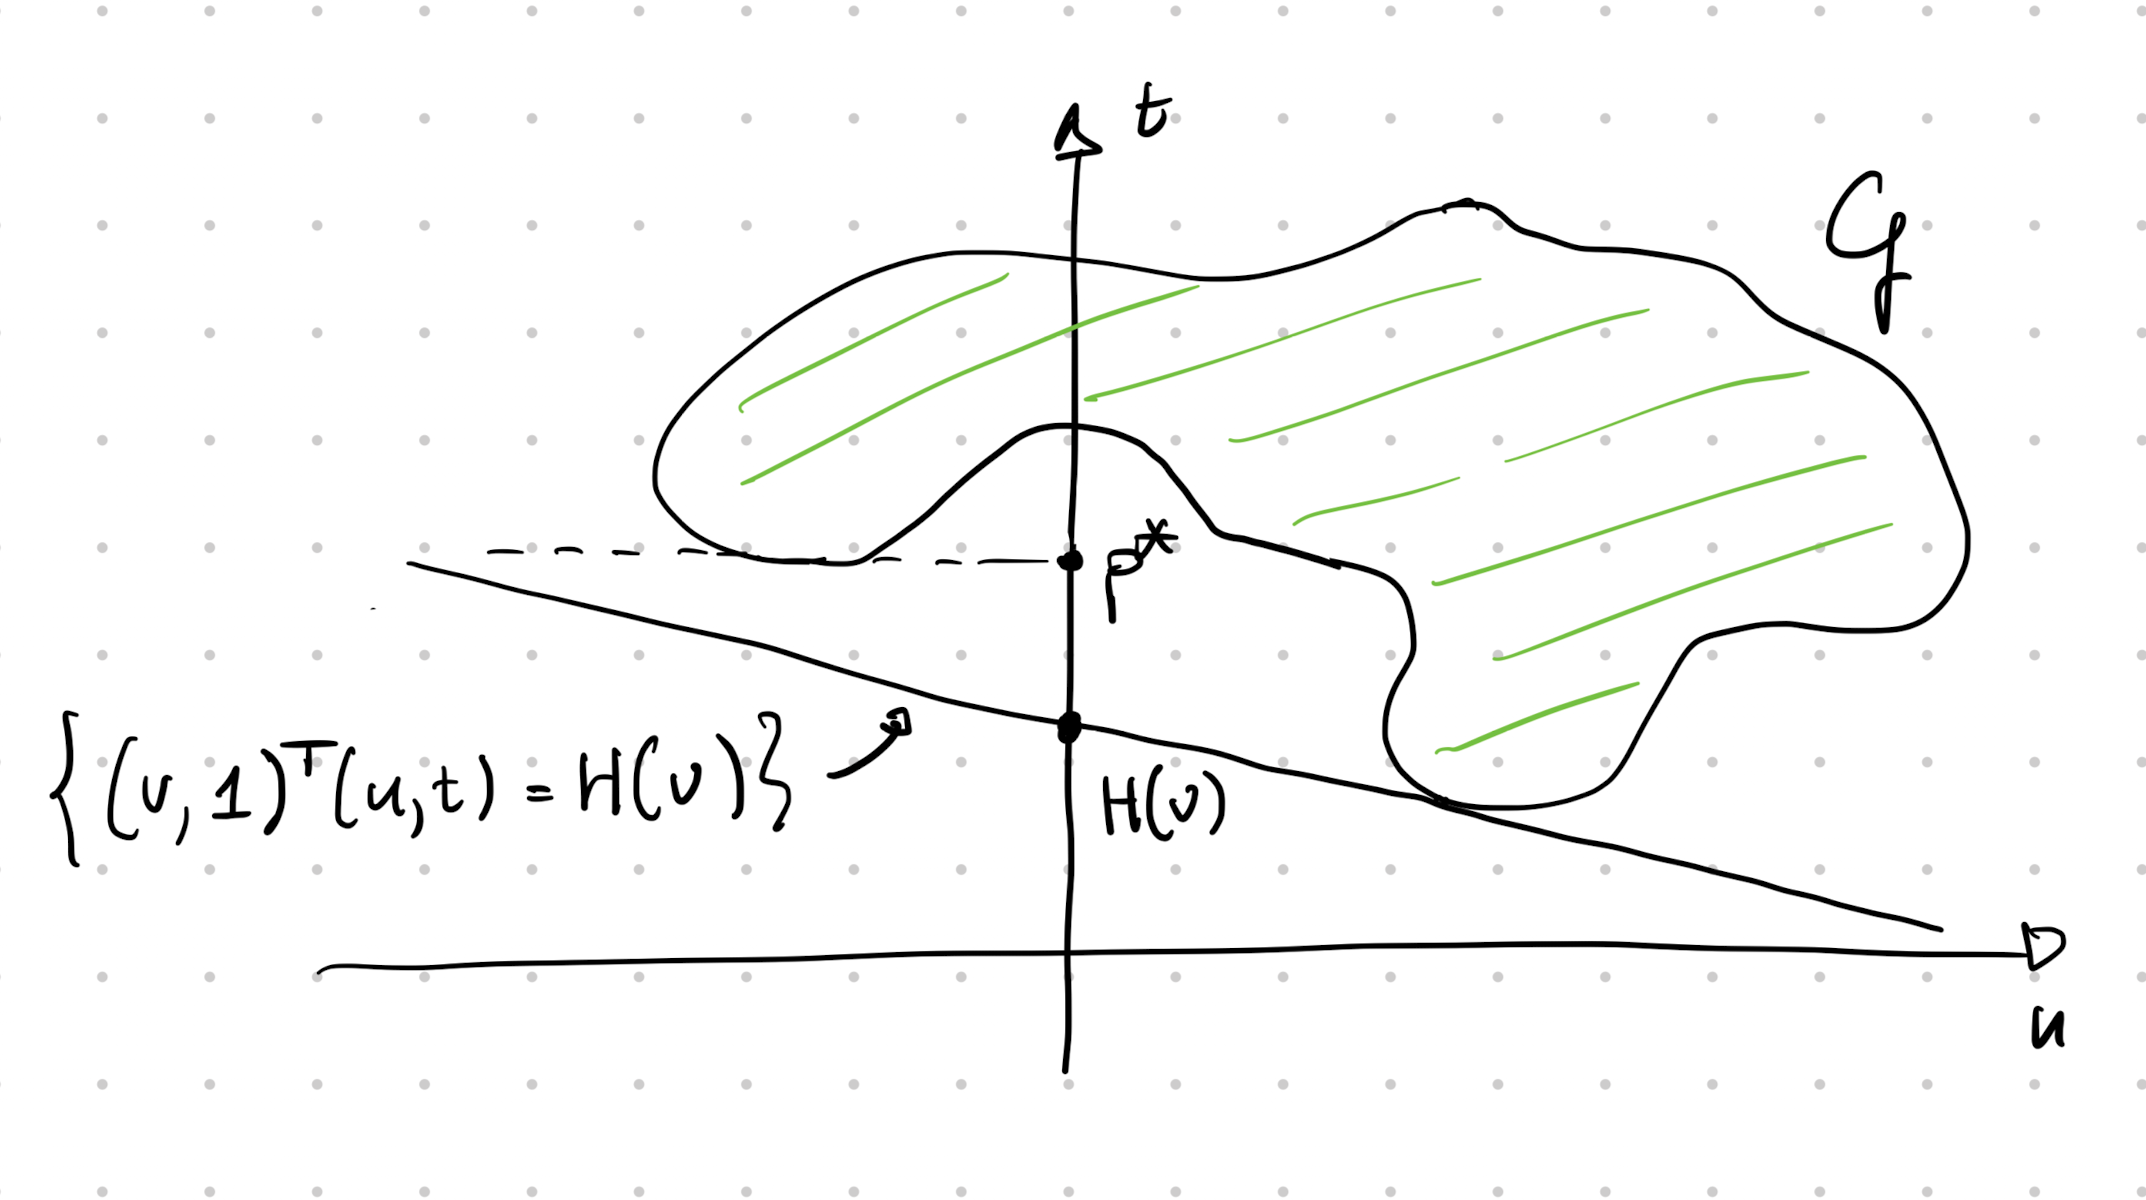
\includegraphics[width=.8\textwidth]{images/geometric-primal-dual-1.png}
             \caption{Geometric interpretation. The value of the dual function $H(\nu)$ identifies a supporting hyperplane for the set $\mcG$.}
             \label{fig:geom1}
         \end{minipage}
         \hfill
         \begin{minipage}{.48\textwidth}
             \centering
             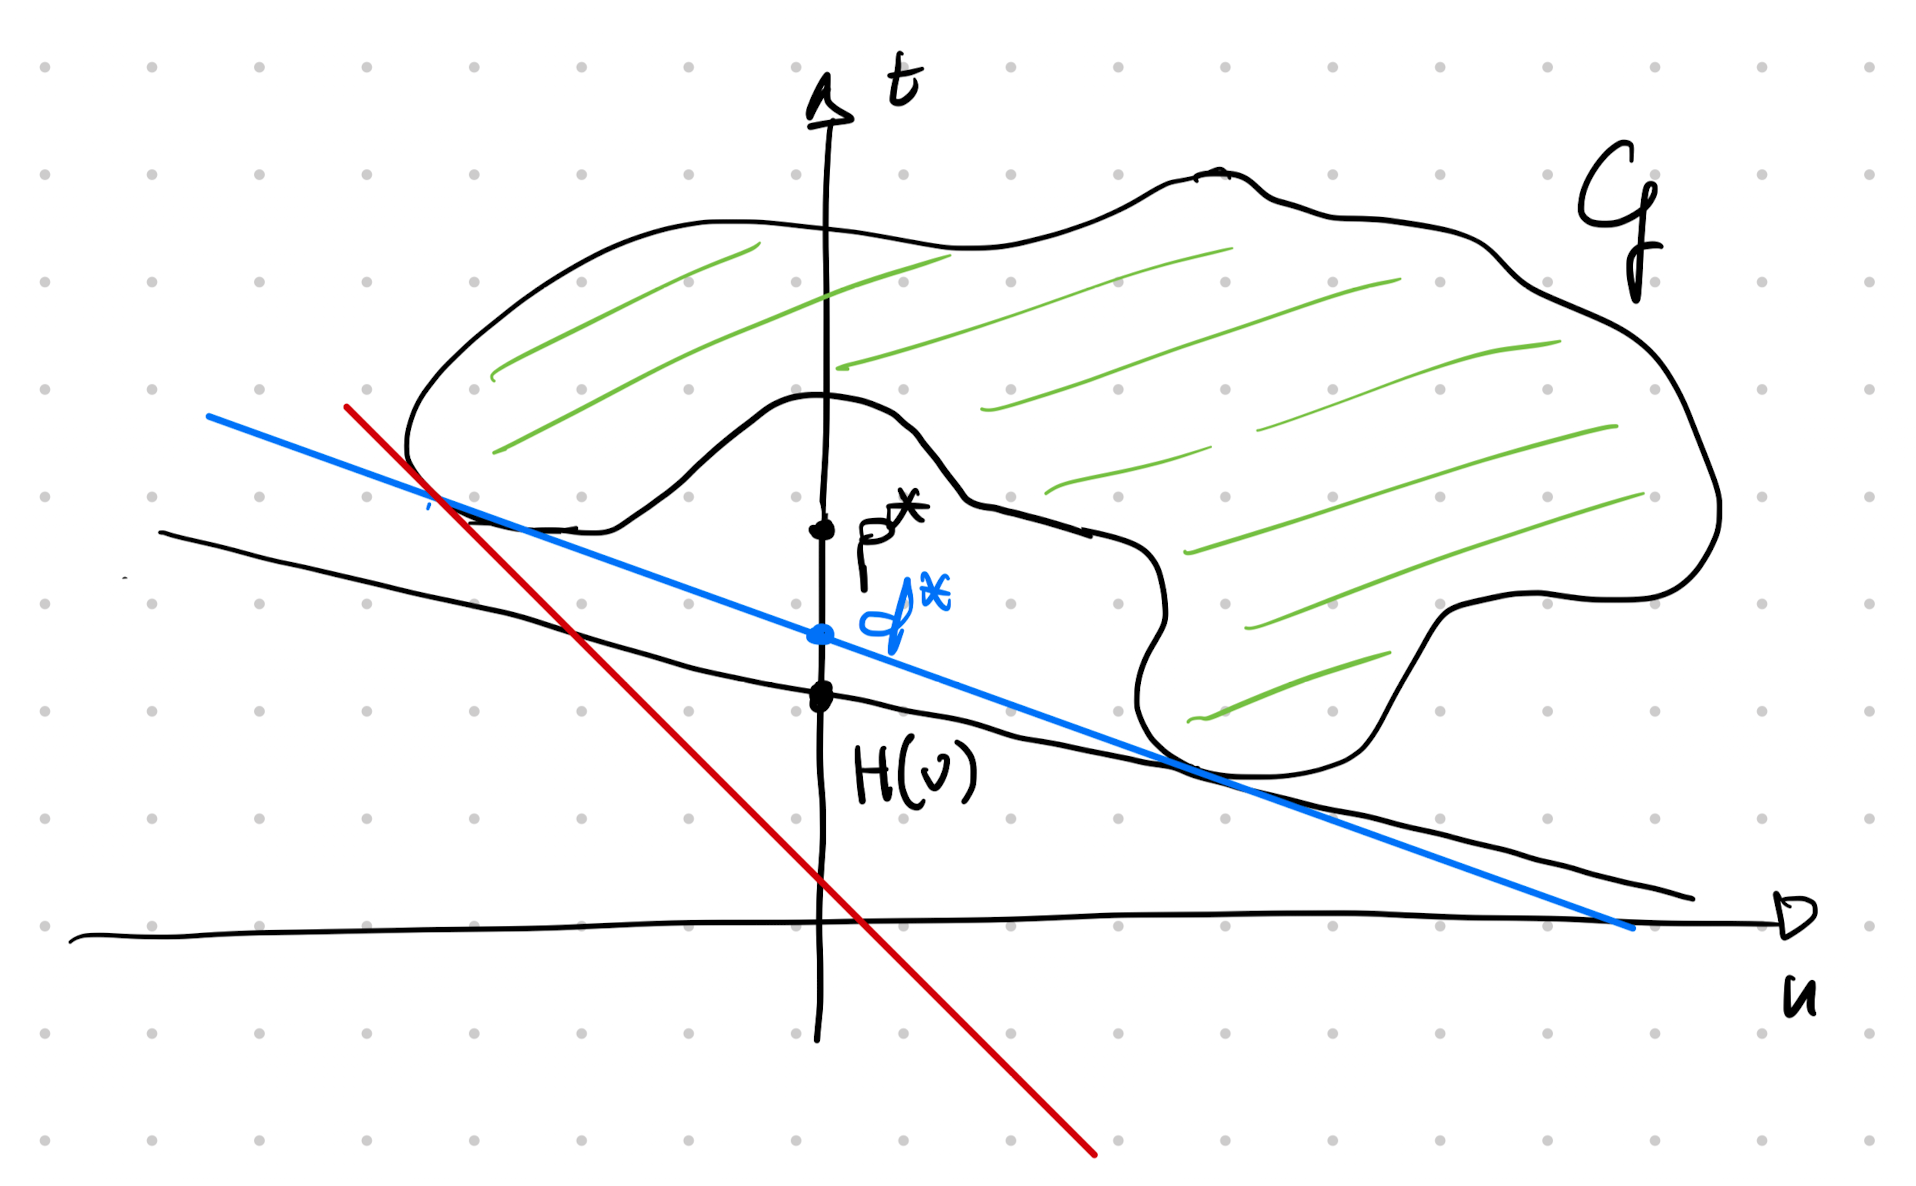
\includegraphics[width=.8\textwidth]{images/geometric-primal-dual-2.png}
             \caption{Geometric interpretation. Solving the dual problem yields the blue hyperplane. In this case $p^\star > d^\star$ and strong duality does not hold.}
             \label{fig:geom2}
         \end{minipage}
         \begin{minipage}{.48\textwidth}
             \centering
             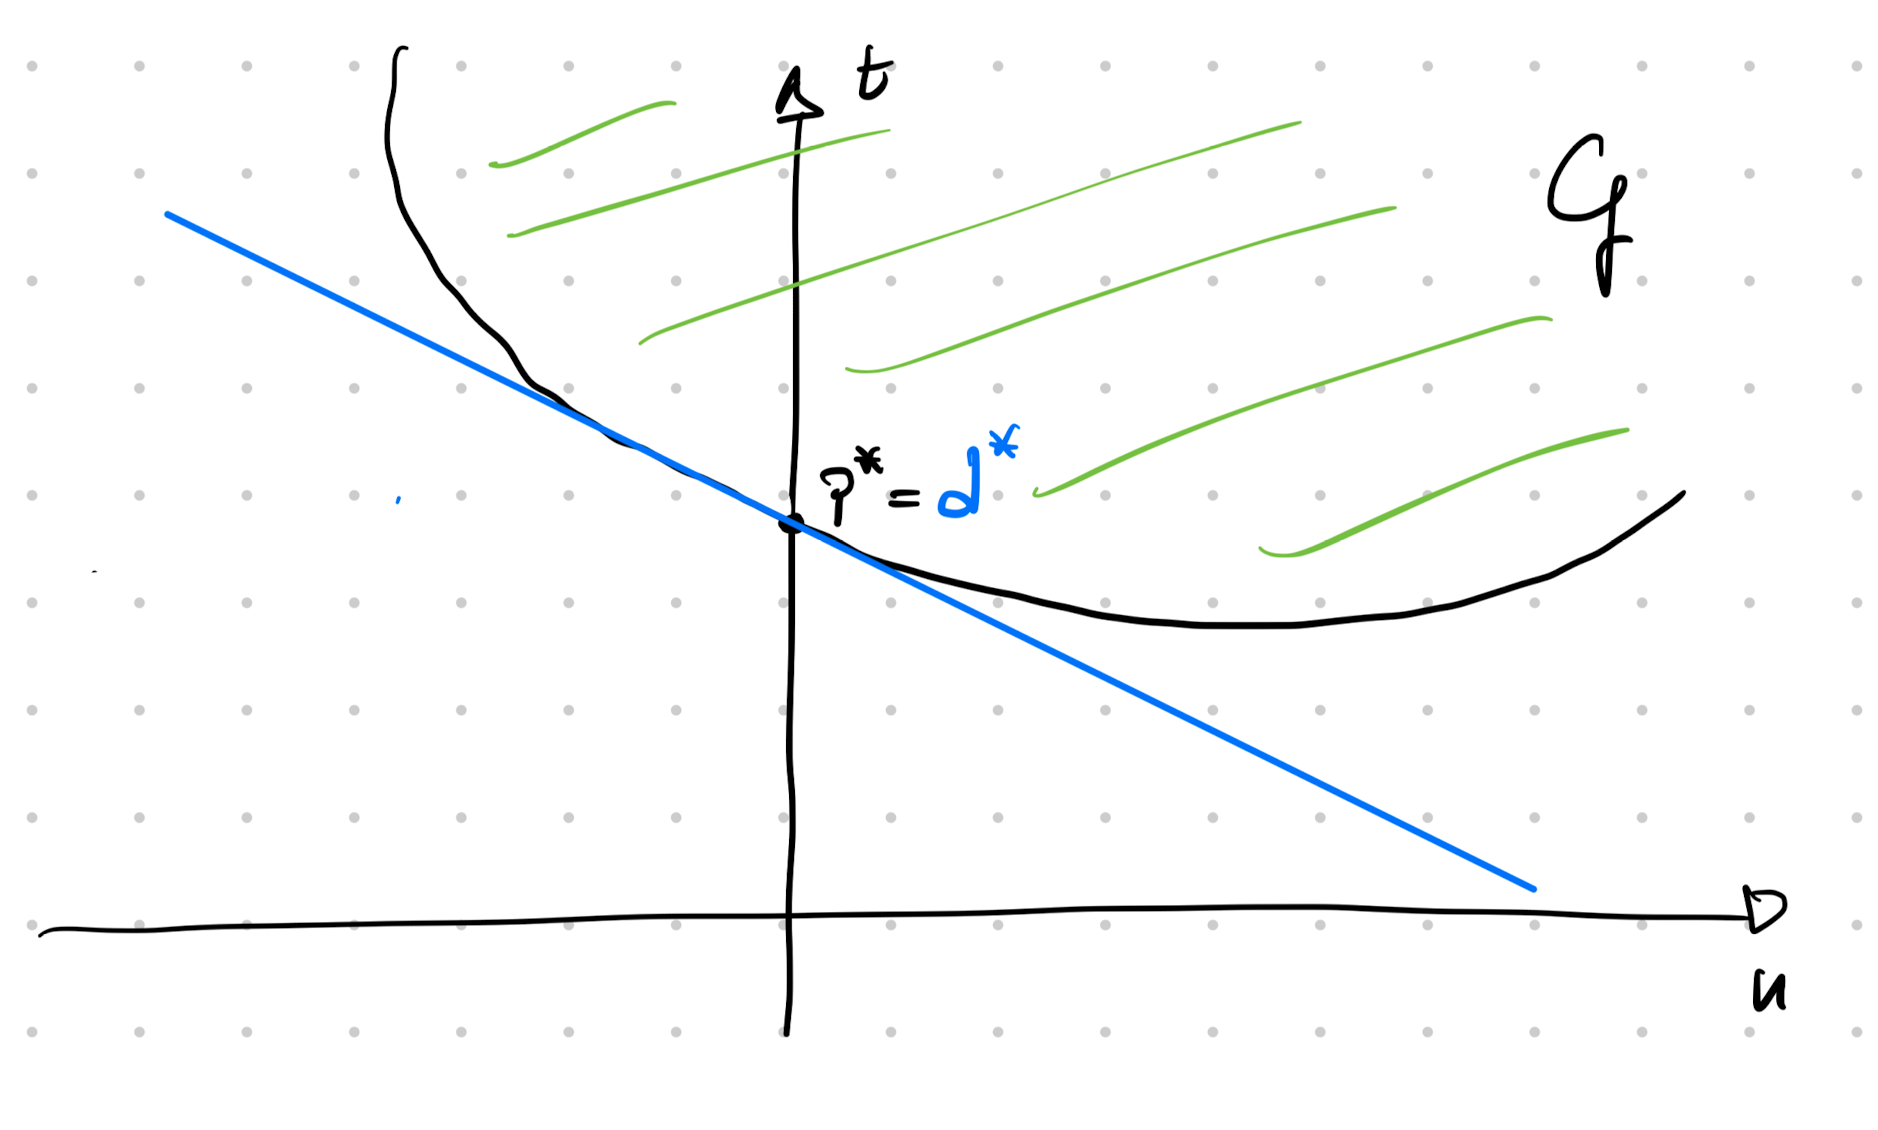
\includegraphics[width=.8\textwidth]{images/geometric-primal-dual-3.png}
             \caption{Geometric interpretation of Slater's condition. When the set $\mathcal G$ is convex and has interior that intersects the left-hand plane, the best supporting hyperplane yields the optimal value $p^\star$.}
             \label{fig:geom3}
         \end{minipage}
     \end{figure}
 
 
     \section{Conic optimization problems}
 
     \dfn{}{
         A \emph{conic optimization problem} is a minimization problem of the form
         \begin{equation}
             \tag{COP}
             \label{eq:cop}
             \min_{x\in \bbR^d} F_0(x)
             \qquad\text{subject to}\qquad
             x\in K
             \qquad \text{and}\qquad
             F_j(x)\le 0, \qquad j\in\llbracket 1, M\rrbracket.
         \end{equation}
         Here, $F_0,\ldots, F_M:\bbR^d\to \bbR\cup\{+\infty\}$ are convex functions and $K\subset \bbR^d$ is a convex cone.
     }
 
     Also conic optimization problems have their duality theory.
 
     \dfn{Duality for conic optimization problems}{
         The \emph{Lagrange function} of the optimization problem \eqref{eq:cop} is the function $F:\bbR^d \times \bbR^m \times \bbR^M_+\to \bbR\cup\{+\infty\}$ defined by
         \begin{equation}
             L(x,\xi,\nu) = F_0(x) - \langle \xi,x\rangle +\sum_{j=1}^m \nu_j F_j(x).
         \end{equation}
 
         The \emph{Lagrange dual function} is the function $H:\bbR^m\times \bbR^M_+ \to \bbR\cup\{-\infty\}\cup\{+\infty\}$, defined by
         \begin{equation}
             H(\xi,\nu) = \inf_{x\in \bbR^d} L(x,\xi,\nu).
         \end{equation}
 
         The dual problem associated with \eqref{eq:cop} is then
         \begin{equation}
             \max_{\xi\in \bbR^m, \nu \in \bbR^M}H(\xi,\nu)
             \qquad\text{subject to}\qquad
             \xi \in K^*,\, \nu\in \bbR_+^M.
         \end{equation}
         Here, $K^*$ is the dual cone of $K$ (see Definition~\ref{def:dual-cone})
     }
 
     The duality theory is set up in order to have weak duality.
 
     \prop[]{}{
         The dual function is always concave. Moreover, if $x^\star$ is a minimizer of \eqref{eq:cop}, we have
         \begin{equation}
             H(\xi,\nu) \le F(x^\star), \qquad \forall \xi\in \bbR^m,\, \nu\in \bbR^M_+.
         \end{equation}
     }
     The proof of this result can be done as for Proposition~\ref{prop:weak-duality}, taking into account the definition of dual cone.
 
     Similar conditions as in Slater's constraint qualification (Theorem~\ref{th:slater}) ensure strong duality for conic problems; for instance, if there exists a point in the interior of K such that all inequality constraints hold strictly, see e.g., \cite[Section~5.9]{boydConvex2023}.
 
     \ex{}{
         For a convex cone $K\subset\bbR^d$ and a vector $v\in \bbR^d$, consider the conic optimization problem
         \begin{equation}
             \min_{x\in\bbR^d} \langle x,v\rangle
             \qquad\text{subject to}\qquad
             x\in K,\, \|x\|_2^2\le 1.
         \end{equation}
 
         The Lagrange function is given by
         \begin{equation}
             L(x,\xi,\nu) = \langle x,v\rangle -\langle \xi,x\rangle +\nu(\|x\|_2^2 - 1), \qquad \xi\in K^*,\, \nu\ge 0.
         \end{equation}
         Minimizing the above w.r.t.~$x$ one immediately obtains
         \begin{equation}
             H(\xi,\nu) = -\nu -\frac{1}{4\nu}\|\xi-v\|_2^2, \qquad \xi\in K^*,\, \nu\ge 0.
         \end{equation}
         For fixed $\xi$ it is easy to maximize $H(\xi,\nu)$ w.r.t.~$\nu\ge 0$, yielding $\nu = \|\xi-v\|_2^2/2$. Thus, the dual problem simplifies to
         \begin{equation}
             \label{eq:dual-example}
             \max_{\xi\in \bbR^m} \left(-\frac{\|\xi-v\|_2}{2}\right)
             \qquad \text{subject to} \qquad
             \xi\in K^*.
         \end{equation}
         That is, the optimal value of the dual problem is the optimal value of the above, and any dual optimal $(\xi^\star,\nu^\star)$ is such that $\nu^\star=\|\xi^\star-v\|_2^2/2$ and $\xi^\star$ is optimal for the above.
 
         Observe, that minimizers for \eqref{eq:dual-example} are the orthogonal projections of $v$ on the dual cone $K^*$.
     }
 
     \section{Saddle-point interepretation and penalty method}
 
 
 
 
     \thm[saddle-point]{Saddle-point property}{
         Consider an optimisation problem (convex of conical). Then, the primal-dual optimal values $p^\star$ and $d^\star$ satisfy
         \begin{equation}
             \label{eq:saddle-point}
             p^\star = \inf_{x\in \bbR^d}\sup_{\xi\in \bbR^m,\, \nu\in \bbR^M_+} L(x,\xi,\nu)
             \qquad\text{and}\qquad
             d^\star = \sup_{\xi\in \bbR^m,\, \nu\in \bbR^M_+} \inf_{x\in \bbR^d} L(x,\xi,\nu).
         \end{equation}
         In particular,
         \begin{itemize}
             \item Strong duality is equivalent to the fact that
                   \begin{equation}
                       \inf_{x\in \bbR^d}\sup_{\xi\in \bbR^m,\, \nu\in \bbR^M_+} L(x,\xi,\nu)
                       =
                       \sup_{\xi\in \bbR^m,\, \nu\in \bbR^M_+}\inf_{x\in \bbR^d} L(x,\xi,\nu).
                   \end{equation}
             \item Primal-dual optimizer $(x^\star,\xi^\star,\nu^\star)$ are exactly the saddle points of $L$. That is,
                   \begin{equation}
                       L(x^\star, \xi,\nu) \le L(x^\star,\xi^\star,\nu^\star)\le L(x,\xi^\star,\nu^\star), \qquad \forall x\in \bbR^d, \, (\xi,\nu)\in \bbR^m\times \bbR^M_+.
                   \end{equation}
         \end{itemize}
     }
 
     \begin{proof}
         We consider a convex optimisation problem (the same considerations hold \emph{mutas mutandis} for conical problems).
 
         The fact that $d^\star$ satisfyies \eqref{eq:saddle-point} is a direct consequence of the definition.
         On the other hand, we have
         \begin{equation}
             \sup_{\xi\in\bbR^m, \nu\in \bbR^M_+} L(x,\xi,\nu) = F_0(x) + \sup_{\xi\in \bbR^m} \langle \xi,Ax-y\rangle + \sup_{\nu_j\ge 0} \sum_{j=1}^M \nu_j F_j(x)
             =
             \begin{cases}
                 F_0(x)  & \text{if } Ax=y\text{ and } F_j(x)\le 0 \, \forall j\in\llbracket1,M\rrbracket, \\
                 +\infty & \text{otherwise}.
             \end{cases}
         \end{equation}
         In other words, the above supremum is $+\infty$ if $x$ is not feasible (i.e., $x\notin\feas$). This shows that minimizing the above w.r.t.~$x\in \bbR^d$ yields $p^\star$.
     \end{proof}
 
     As a consequence of the saddle-point property, we recover a classical method (penalty method or Tychonoff regularization), that allows to transform constrained problems in different but equivalent unconstrained problems that are typically easier to solve.
 
     Given two parameters $\eta> 0$ and $\lambda \ge 0$, we consider the following two problems:
     \begin{equation}
         \label{eq:op-eta}
         \tag{PO$_2$($\eta$)}
         \min_{x\in\bbR^d}F_0(x)
         \qquad\text{subject to}\qquad
         F_1(x)\le \eta,
     \end{equation}
     and
     \begin{equation}
         \label{eq:op-lambda}
         \tag{PO$_2$($\lambda$)}
         \min_{x\in\bbR^d}F_0(x) + \lambda F_1(x).
     \end{equation}
 
     We have the following.
 
     \thm{Penalty method}{
         % Assume that \eqref{eq:op-eta} is strictly feasible, in the sense that there exists $x^\star\in\bbR^d$ such that $F_1(x^\star)<\eta$. 
         Assume that $F_0,F_1$ are lower semicontinuous, satisfy the assumptions of Theorem~\ref{th:slater}, and that $F_1(x)\ge 0$ for all $x\in \bbR^d$.
         Then, for $x^\star\in \bbR^d$ the following statements are equivalent:
         \begin{itemize}
             \item There exists $\eta\ge 0$ such that $x^\star$ is a minimizer of \eqref{eq:op-eta}.
             \item There exists $\lambda\ge 0$ such that $x^\star$ is a minimizer of \eqref{eq:op-lambda}.
         \end{itemize}
     }
 
     \begin{proof}
         Assume that $x^\star$ is a minimizer for \eqref{eq:op-eta}, and recall that for this problem
         \begin{equation}
             L(x,\nu) = F_0(x) +\nu (F_1(x)-\eta), \qquad x\in \bbR^d,\, \nu\ge 0.
         \end{equation}
         By Theorem~\ref{th:slater}, we have that strong duality holds for \eqref{eq:op-eta} and that there exists a primal-dual optimal $(x^\star,\nu^\star)$. By the saddle-point propery (Theorem~\ref{th:saddle-point}) it holds that $L(x^\star, \nu^\star)\le L(x, \nu^\star)$ for any $x \in\bbR^d$. Since the constant term $-\nu^\star\eta$ does not affect the minimization, this proves that $x^\star$ is a minimizer of \eqref{eq:op-lambda} with $\lambda=\nu$.
 
         For the converse statement, assume now that $x^\star$ is a minimizer of \eqref{eq:op-lambda}.
         Choose $\eta = F_1(x^\star)\ge 0$, so that the dual function of problem \eqref{eq:op-eta} satisfies
         \begin{equation}
             H(\lambda) = \inf_{x\in \bbR^d} L(x, \lambda) = \inf_{x\in \bbR^d} \left[ F_0(x) +\lambda F_1(x) \right] - \lambda F_1(x^\star)
             = F_0(x^\star).
         \end{equation}
         Here, we used that $x^\star$ is a minimizer for \eqref{eq:op-lambda}.
         % Observe that here we used the non-negativity of $F_1$.
         Since weak duality implies that $H(\lambda)\le F_0(x)$ for any feasible $x\in \bbR^d$, and $x^\star$ is feasible due to the choice of $\eta$, it follows that $x^\star$ is a minimizer of \eqref{eq:op-eta}.
     \end{proof}
 
     \begin{remark}
         The non-negativity assumption on $F_1$ can be removed by replacing $F_1(x)$ in \eqref{eq:op-lambda} by $\min\{0,F_1(x)\}$.
     \end{remark}
 
 
 
     % \dfn{Definition Topic}{Definition Statement}
     % \thm{Theorem Name}{Theorem Statement}
     % \cor[cori]{Corollary Name}{Corollary Statement}
     % \lem{Lemma Name}{Lemma Statement}
     % \clm{Claim Name}{Claim Statement}
     % \ex{Example Name}{Example explained}
     % \opn{Open Question Name}{Question Statement}
     % \qs{Question Name}{Question Statement}
     % \nt{Special Note}
     % \wc{Wrong Concept topic}{Explanation}
     % \pf{Proof}{Proof}
 
     \chapter{Numerical methods for (non)convex optimization}
 
     \section{Gradient descent}
 
     We are concerned with the following unconstrained minimization problem
     \begin{equation}
         \label{eq:unc-opt}
         \min_{x\in\bbR^d} f(x),
     \end{equation}
     where $f:\bbR^d\to \bbR$ is a sufficiently smooth (say $C^1$) function.
 
     Since the gradient $\nabla f(x)$ encodes the direction of maximal growth of $f$ at $x$, it is natural to expect that moving in the direction $-\nabla f(x)$ will lead to a minimum $x^\star$ \eqref{eq:unc-opt}.
 
     \dfn{Gradient flow}{
         Assume that $f\in C^1(\bbR^d)$.
         The associated gradient flow from $x_0\in \bbR^d$ is ordinary differential equation:
         \begin{equation}
             \label{eq:grad-flow}
             \dot x = -\nabla f(x), \qquad x(0)=x_0.
         \end{equation}
     }
 
     By Cauchy-Lipschitz theorem, \eqref{eq:grad-flow} admits local solutions.
     In order for them to be global, we assume the following.
 
     \ass[grad-lip]{}{
         The function $f\in C^{1}(\bbR^d)$ and, moreover, $\nabla f:\bbR^d\to \bbR^d$ is Lipschitz continuous with constant $L>0$. That is,
         \begin{equation}
             \label{eq:grad-lip}
             \|\nabla f(x)-\nabla f(y)\|_2 \le L \|x-y\|_2,\qquad \forall x,y\in\bbR^d.
         \end{equation}
     }
 
     Observe that if $f\in C^2(\bbR^d)$, the above assumption is verified by assuming that $\operatorname{Hess} f(x)\le L \operatorname{Id}$ in the sense of symmetric matrices (i.e.,  all eigenvalues of $\operatorname{Hess}f(x)$ are bounded above by $L$).
 
     Recall also that a function $f\in C^2(\bbR^d)$ that is strongly convex (i.e., there exists $\gamma>0$ such that $\operatorname{Hess}f(x)\ge \gamma/2$ for any $x\in \bbR^d$) always admits a unique minimizer (see Proposition~\ref{prop:convexity-diff} and Theorem~\ref{th:min-convex}).
 
     \thm[conv-grad-flow]{}{
         Assume that $f\in C^2(\bbR^d)$ is strongly convex function satisfying Assumption~\ref{ass:grad-lip}.
         Then, for any initial condition $x_0\in \bbR^d$, the gradient flow \eqref{eq:grad-flow} converges to the unique minimizer $x^\star = \arg\min_{x\in\bbR^d} f(x)$.
     }
 
     \begin{proof}
         Since $x^\star$ is unique, it is characterized by property $\nabla f(x^\star)=0$. In particular, the statement is trivial if $x_0=x^\star$.
         Otherwise, let $V(x) = \frac12\|\nabla f(x)\|_2^2$ and observe that $\nabla V(x) = \operatorname{Hess}f(x) \nabla f(x)$. Computing $V$ along a solution $t\mapsto x(t)$ of \eqref{eq:grad-flow} we have
         \begin{equation}
             \begin{split}
                 \frac{d}{dt}V(x(t))
                  & = \nabla V(x(t))^\top \dot x(t)                                  \\
                  & = \nabla f(x(t))^\top \operatorname{Hess}f(x(t)) \dot x(t)       \\
                  & = -\nabla f(x(t))^\top \operatorname{Hess}f(x(t)) \nabla f(x(t)) \\
                  & \le -\frac{\gamma}2 \|\nabla f(x(t))\|_2^2 = -\gamma V(x(t)).
             \end{split}
         \end{equation}
         Here, we used the fact that $\operatorname{Hess}f(x)\ge \gamma/2$.
         By integration of the above, we then obtain that for any $t\ge 0$ it holds
         \begin{equation}
             V(x(t)) \le V(x_0)e^{-\gamma t}
             \iff
             \|\nabla f(x(t))\|_2\le \|\nabla f(x_0)\|_2 e^{-\gamma t/2}.
         \end{equation}
         Recall that $\nabla f(x^\star)=0$, this implies that
         \begin{equation}
             \label{eq:estimate-grad}
             \lim_{t\to +infty} \|\nabla f(x(t)) - \nabla f(x^\star)\|_2 \le \|\nabla f(x_0)\|_2 \lim_{t\to +\infty} e^{-\gamma t/2} = 0.
         \end{equation}
 
         Let us now use the above to show that $x(t)\rightarrow x^\star$ as $t\to +\infty$.
         Indeed, we have
         \begin{equation}
             \begin{split}
                 \frac{d}{dt}\frac12\|x(t)-x^\star\|_2^2
                  & = \langle x(t)-x^\star, \dot x(t) \rangle                             \\
                  & = -\langle x(t)-x^\star, \nabla f( x(t)) \rangle                      \\
                  & = -\langle x(t)-x^\star, \nabla f( x(t)) - \nabla f(x^\star) \rangle.
             \end{split}
         \end{equation}
         By Theorem~\ref{th:co-coercivity}, to be proven later, this implies
         \begin{equation}
             \frac{d}{dt}\frac12\|x(t)-x^\star\|_2^2
             \le -\frac{1}{L} \|\nabla f(x(t))-\nabla f(x_0)\|_2^2
             \le 0.
         \end{equation}
         Integrating the above, we obtain $\|x(t)-x^\star\|_2 \le \|x_0-x^\star\|_2$, which implies that $x(t)\in \bar B(x^\star, \|x_0-x^\star\|_2)$ (i.e., the evolution $t\mapsto x(t)$ is uniformly bounded in time).
         By compactness, there exists a sequence of times $(t_n)_n\subset \bbR_+$ and a point $x_\infty$ such that $x(t_n)\rightarrow x_\infty$.
         However, the fact that $f\in C^2(\bbR^d)$ implies that $\nabla f(x(t_n))\rightarrow \nabla f(x_\infty)$, and thus  \eqref{eq:estimate-grad} yields that $\nabla f(x_\infty) = \nabla f(x^\star)=0$.
         By existence and uniqueness of the minimizer of $f$, this shows that $x_\infty=x^\star$.
     \end{proof}
 
     \thm[co-coercivity]{Co-coercivity}{
         Let $f\in C^1(\bbR^d)$ be convex and such that $\nabla f$ is Lipschitz continuous with constant $L>0$. Then, we have that
         \begin{enumerate}
             \item Quadratic upper bound (compare with Proposition~\ref{prop:convexity-diff}, this does not require convexity):
                   \begin{equation}
                       \label{eq:quad-low-bound}
                       f(y) \le f(x) + \langle \nabla f(x), y-x \rangle + \frac{L}2 \|y-x\|^2, \qquad \forall x,y\in \bbR^d.
                   \end{equation}
             \item If $x^\star$ is a minimizer for $f$,
                   \begin{equation}
                       \label{eq:previous}
                       \frac{1}{2L}\|\nabla f(y)\|_2^2 \le f(y) - f(x^\star) \le \frac{1}{2}\|y-x^\star\|_2^2, \qquad \forall y\in \bbR^d.
                   \end{equation}
             \item Co-coercivity:
                   \begin{equation}
                       \|\nabla f(x)-\nabla f(y)\|_2^2\le L \langle x-y, \nabla f(x)-\nabla f(y) \rangle,
                       \qquad \forall x,y\in \bbR^d.
                   \end{equation}
         \end{enumerate}
     }
 
     \begin{proof}
         The quadratic upper bound is a direct consequence of the fact that
         \begin{equation}
             f(y)
             =f(x)+\int_0^1 \frac{d}{dt} f(x+t(y-x)) \, dt
             =f(x)+\int_0^1 \langle\nabla f(x+t(y-x)), y-x \rangle\, dt.
         \end{equation}
         Indeed, the $L$-Lipschitz property of $\nabla f$ and the Cauchy-Schwarz inequality yields
         \begin{equation}
             \langle\nabla f(x+t(y-x)), y-x \rangle
             \le \langle\nabla f(x), y-x \rangle + L \|y-x\|^2.
         \end{equation}
 
         To prove the second part of the statement, since $\nabla f(x^\star) =0$ the right-hand inequality follows from the quadratic lower bound \eqref{eq:quad-low-bound} with $x=x^\star$. On the other hand, still by \eqref{eq:quad-low-bound} with $x=y$ and $y=z$ we obtain
         \begin{equation}
             \begin{split}
                 f(x^\star)
                  & = \inf_{z} f(z)                                                                                        \\
                  & \le \inf_z \left[ f(y) + \langle \nabla f(y), z-y \rangle + \frac{L}2 \|y-z\|^2 \right]                \\
                  & \le \inf_{\|v\|=1} \inf_{t\ge 0} \left[ f(y) + t\langle \nabla f(y), v \rangle + \frac{Lt^2}2  \right] \\
                  & = \inf_{\|v\|=1} \left[ f(y) - \frac{1}{2L} \left(\langle \nabla f(y),x\rangle\right)^2 \right]        \\
                  & = f(y) - \frac{1}{2L} \|\nabla f(y)\|_2^2.
             \end{split}
         \end{equation}
 
         To conclude the proof, let us fix $x\in \bbR^d$ and consider the two functions
         \begin{eqnarray}
             f_x(z) = f(z)-\langle \nabla f(x),z\rangle
             \qquad\text{and}\qquad
             f_y(z) = f(z)-\langle \nabla f(y),z\rangle.
         \end{eqnarray}
         It is immediate to check that $\nabla f_x(z) = \nabla f(z)-\nabla f(x)$ is Lipschitz continuous of constant $L$, and that $f_x$ is convex.
         Since $z=x$ minimizes $f_x$ by convexity, the left-hand inequality in \eqref{eq:previous} applied to $f_x$ at $x^\star =x$ shows that
         \begin{equation}
             f(y)-f(x)-\langle \nabla f(x),y-x \rangle = f_x(y)-f_x(x) \ge \frac{1}{2L}\|\nabla f_x(y)\|_2^2 = \frac{1}{2L}\|\nabla f(y)-\nabla f(x)\|_2^2.
         \end{equation}
         The same reasoning applied to $f_y$, which is minimized by $z=y$, yields
         \begin{equation}
             f(x)-f(y)-\langle \nabla f(y),x-y \rangle \ge \frac{1}{2L}\|\nabla f(y)-\nabla f(x)\|_2^2.
         \end{equation}
         Combining the two inequalities completes the proof.
     \end{proof}
 
     A natural time-discretization of the gradient flow \eqref{eq:grad-flow} is via the Explicit Euler scheme, which yields the gradient descent algorithm.
 
     \dfn[grad-desc]{Gradient descent algorithm}{
         The gradient descent algorithm for $f\in C^1(\bbR^d)$ starting at $x_0\in \bbR^d$ with parameters $(\alpha_n)_n\subset \bbR_+$, is
         \begin{equation}
             \label{eq:discr-grad-desc}
             x_{n+1} = x_n - \alpha_n \nabla f(x_n).
         \end{equation}
     }
 
     Here the parameters $\alpha_n$ are tyipically chosen adaptively with a line search. However, also a constant choice $\alpha = \alpha_n$ sufficiently small will suffice. Let us show now a result of convergence of the algorithm above.
 
     \thm[grad-desc]{}{
         Let $f\in C^1(\bbR^d)$ be coercive (i.e., $f(x)\to +\infty$ as $x\to +\infty$), and such that $\nabla f$ is Lipschitz continuous with constant $L>0$, and admitting a unique minimizer $x^\star$.
         Assume that
         \begin{equation}
             \sum_{n=0}^{+\infty} \alpha_n = +\infty
             \qquad\text{and}\qquad
             \alpha_n \le \frac{1}L,\quad
             \forall n\in \bbN.
         \end{equation}
         Then, the iterations of the algorithm \eqref{eq:discr-grad-desc} converge to $x^\star$ (i.e., $x_n\rightarrow x^\star$ as $n\to +\infty$).
     }
 
     \begin{proof}
         Fix $n\in\bbN$.
         % To ease the notation, set $x=x_n$, $\alpha = \alpha_n$, and $x^+=x_{n+1}=x-\alpha \nabla f(x)$. 
         Then, by the quadratic upper bound of Theorem~\ref{th:co-coercivity}, we have
         \begin{equation}
             \label{eq:first-step1}
             f(x_{n+1})
             \le f(x_n) + \langle \nabla f(x_n), x_{n+1}-x_n \rangle+\frac{L}2\|x_{n+1}-x_n\|_2^2
             = f(x_n)-\alpha_n \left(1-\frac{\alpha_n L}2\right) \|\nabla f(x_n)\|_2^2.
         \end{equation}
 
         The above implies that
         \begin{equation}
             \sum_{n=0}^{N-1} \alpha_n \left(1-\frac{\alpha_n L}2\right) \|\nabla f(x_n)\|_2^2 \le \sum_{n=0}^{N-1} \left(f(x_{n})-f(x_{n+1})\right) =f(x_0) - f(x_N) \le f(x_0)-f(x^\star).
         \end{equation}
         Since the r.h.s.~is independent of $N$ and $(1-L\alpha_n/2) \ge 1/2$, this shows that
         \begin{equation}
             \sum_{n=0}^{N-1} \alpha_n  \|\nabla f(x_n)\|_2^2 \le
             \frac12\sum_{n=0}^{N-1} \alpha_n \left(1-\frac{\alpha_n L}2\right) \|\nabla f(x_n)\|_2^2 < +\infty.
         \end{equation}
         Since $\sum_n \alpha_n = +\infty$ by assumption, one easily shows by contradiction that $\|\nabla f(x_n)\|_2\rightarrow 0$ as $n\to +\infty$.
 
         Observe that, by \eqref{eq:first-step1} and the assumption $\alpha_n\le 1/L$, we deduce that $f(x_{n+1})<f(x_n)$ for any $n\in \bbN$. In particular, by coercivity, there exists $R>0$ such that $x_n\in \bar B(0,R)$ for any $n\in \bbN$, and thus the same argument used at the end of the proof of Theorem~\ref{th:conv-grad-flow} shows that $\|\nabla f(x_n)\|_2^2$ implies convergence to the unique minimum.
     \end{proof}
 
     \begin{remark}
         The coercivity assumption can be relaxed by simply asking that the level set $\{x\mid f(x)\le f(x_0)\}$ be bounded.
         Is it also possible to remove the assumption of uniqueness of the minimum, in which case we have that every cluster point of the iterates is a minimum.
     \end{remark}
 
     Under additional assumptions on the function $f$, we can quantify its the rate of convergence.
 
     \thm[]{}{
         Under the assumptions of Theorem~\ref{th:grad-desc}, letting $\alpha_n = \alpha \le 1/L$, we have
         \begin{itemize}
             \item If $f$ is convex, the convergence is \emph{sublinear}: there exists $c>0$ such that
                   \begin{equation}
                       \label{eq:grad-desc-convex}
                       f(x_n)-f(x^\star) \le c{\|x_0-x^\star\|_2^2}
                   \end{equation}
             \item If $f$ is $\gamma$-strongly convex, the convergence is \emph{exponential}: there exists $c>0$ and $\mu\in(0,1)$ such that
                   \begin{equation}
                       \|x_n-x^\star\|_2 \le \mu^n\|x_0-x^\star\|_2, \qquad\forall n\in\bbN.
                   \end{equation}
         \end{itemize}
     }
 
     \begin{proof}
         By definition of $x_{n+1}$ we have
         \begin{equation}
             \label{eq:cosine-thm}
             \|x_{n+1}-x^\star \|_2^2
             = \|x_n - x^\star\|_2^2 - 2 \alpha \langle \nabla f(x_n),x_n-x^\star \rangle  + \alpha^2 \|\nabla f(x_n)\|_2^2 .
         \end{equation}
         Let us start by assuming that $f$ is convex, so that
         \begin{equation}
             f(x_n)-f(x^\star) \le \langle \nabla f(x_n), x_n-x^\star \rangle
             = \frac{1}{2\alpha} \left[ \|x_n - x^\star\|_2^2 + \alpha^2 \|\nabla f(x_n)\|_2^2  \right].
         \end{equation}
         Applying point 2 of Theorem~\ref{th:co-coercivity} to bound the gradient term, we thus get
         \begin{equation}
             \left(1-{\alpha}{L}\right) f(x_n)-f(x^\star) \le \frac{1}{2\alpha}\|x_n - x^\star\|_2^2 .
         \end{equation}
         Since $1-{\alpha}{L}> 0$, the statement follows by a recursion argument.
 
         Let us now assume that $f$ is $\gamma$-strongly convex. Using the fact that $\nabla f(x^\star)=0$, from the differential characterization of convexity (Theorem~\ref{prop:convexity-diff}) we obtain
         \begin{equation}
             \langle\nabla f(x_n),x_n-x^\star\rangle \ge \frac\gamma2\|x_n-x^\star\|_2^2.
         \end{equation}
         Hence, using also \eqref{eq:grad-lip}, from \eqref{eq:cosine-thm} we obtain
         \begin{equation}
             \|x_{n+1}-x^\star \|_2^2 \le \mu(\alpha)\|x_n - x^\star\|_2^2, \qquad \mu(\alpha) = 1 - \alpha \gamma + \alpha^2 L^2  .
         \end{equation}
         One easily checks that $\mu(\alpha)\in (0,1)$ for $\alpha\in (1,L^{-1})$. The statement follows by a recursion argument.
     \end{proof}
 
     \section{Stochastic gradient descent}
 
     For this section, we mainly refer to \cite{royerLecture}.
 
     The gradient descent algorithm of Definition~\ref{def:grad-desc} is simple to implement and widely used in machine learning. However, it requires to be able to compute $\nabla f(x)$ fairly efficiently at any point $x\in\bbR^d$.
 
     A situation frequently encountered in machine learning is when the objective function is of the form
     \begin{equation}
         \label{eq:loss}
         f(x) = \bbE \left[f(x,\cdot)\right] = \int_\Omega f(x,\omega)\, d\bbP(\omega),
     \end{equation}
     where $f(x,\cdot):\Omega\to \bbR$ are all random variables over a probability space $(\Omega,\mcF, \bbP)$.
     This probability space tipically represents the space of training data: each realization $f(\cdot,\omega)$ is a loss function on the specific sample $\omega\in \Omega$: it tells ``how bad'' picking the parameter $x\in\bbR^d$ for our model performs on this sample.
     Since $\Omega$ can be extremely large,  the computation of
     \begin{equation}
         \label{eq:full-grad}
         \nabla f(x) = \int_{\Omega} \nabla f(x,\omega) \, d\bbP(\omega),
     \end{equation}
     can become extremely expensive and the implementation of a gradient descent unreasonable.
     This is known as the \emph{curse of dimensionality}.
 
     \ex{}{
         If we are trying to learn a regression model, $\omega = (\hat z, \hat y)$ would be the observations, and the model would be $y=mz+q$, with parameter $x=(m,q)$.
         Then, the loss function for the sample $(\hat z,\hat y)$ is
         \begin{equation}
             \ell((m,q),(\hat z, \hat y)) = ( \hat y- m\hat z - q )^2.
         \end{equation}
         The final loss function over $N$ samples is then
         \begin{equation}
             \ell((m,q)) = \frac1N \sum_{i=1}^N \ell((m,q),(\hat z_i,\hat y_i)) = \frac{1}{N}\sum_{i=1}^N ( \hat y_i- m\hat z_i - q )^2.
         \end{equation}
 
         In this case, $\Omega = \{(\hat z_i,\hat y_i) \mid i\in \llbracket 1 ,N\rrbracket\}$ endowed with a uniform probability.
     }
 
     For this particular setting, there is a way out which stems from replacing the actual gradient $\nabla f(x)$ with a ``stochastic approximation'', obtained by sampling \eqref{eq:full-grad}.
 
     \dfn{Stochastic gradient descent}{
         Let $f$ be given as in \eqref{eq:loss}, with $f(\cdot,\omega)\in C^1(\bbR^d)$ for any $\omega\in \Omega$. The stochastic gradient descent algorithm starting at $x_0\in\bbR^d$ with parameters $(\alpha_n)_n\subset \bbR_+$ is
         \begin{equation}
             \label{eq:stoc-grad-desc}
             x_{n+1} = x_n -\alpha_k \nabla_x f(x_n,\omega_n),
         \end{equation}
         where $(\omega_n)_n\in \Omega$ is a sequence of indipendent and identically distributed random variables.
     }
 
     Due to the randomness in the choice of $\omega_n$, this algorithm is probabilistic. We can, however, control its average behavior. For this we need to require certain assumptions on the stochastic gradient.
 
     \ass[stoc-grad]{}{
         At any iteration $n\in \bbN$ of \eqref{eq:stoc-grad-desc}, the random variable $\omega_n$ satisfies
         \begin{enumerate}
             \item The stochastic gradient $\nabla f(x,\omega_n)$ is an unbiased estimator of the real gradient, meaning that $\bbE_{\omega_n}\left[ \nabla f(x,\omega_n) \right] = \nabla f(x)$ for any $x\in \bbR^d$.
             \item There exists $\sigma^2$ such that the following variance estimate holds
                   \begin{equation}
                       \bbE_{\omega_n}\left[ \|\nabla f(x,\omega_n)\|_2^2\right] \le \|\nabla f(x)\|_2^2 + \sigma^2,\qquad \forall x\in \bbR^d.
                   \end{equation}
         \end{enumerate}
     }
 
     \begin{remark}
         In the above, one has to pay attention to the fact that $\nabla f(x,\omega_n)$ is a random variable through $\omega_n$. E.g., in the case where $\Omega$ is discrete
         \begin{equation}
             \bbE_{\omega_n}\left[ \nabla f(x,\omega_n)\right] = \sum_{\omega \in \Omega} \nabla f(x,\omega) \bbP(\omega_n=\omega).
         \end{equation}
     \end{remark}
 
     \ex{Uniform sampling}{
         In the case where $\Omega = \llbracket 1,N\rrbracket$ and $\omega_n$ is just a uniform sampling over $\Omega$ (i.e., $\bbP(\omega_n=k)=1/N$ for any $k\in \Omega$), we have
         \begin{equation}
             \bbE_{\omega_n}\left[ \nabla f(x,\omega_n) \right] = \sum_{k=1}^N 	\nabla f(x,k) \bbP(\omega_n=k) = \frac{1}{N} \sum_{k=1}^N \nabla f(x,k) = \nabla f(x).
         \end{equation}
         In particular, this shows that the first requirement above is always satisfied in this case.
     }
 
     Under these assumptions we have the following.
 
     \prop[estimate-stoc-grad]{}{
         The objective function $f$ in \eqref{eq:loss} is $C^1(\bbR^d)$, strongly convex, and such that $\nabla f$ is Lipschitz continuous with constant $L>0$.
         Moreover, assume that Assumption~\ref{ass:stoc-grad} holds.
 
         Then, the $n$-th iterate of the stocastich gradient descent satisfies
         \begin{equation}
             \bbE_{\omega_n} [f(x_{n+1})] \le  f(x_n) - \alpha_n\left( 1 - \frac{L\alpha_n}{2}\right)\|\nabla f(x_n)\|_2^2+\frac{L\alpha_n}{2}\sigma^2.
         \end{equation}
     }
 
     \begin{proof}
         Fix $n\in\bbN$.
         Then, by the quadratic upper bound of Theorem~\ref{th:co-coercivity}, we have
         \begin{equation}
             \label{eq:first-step}
             f(x_{n+1})
             \le f(x_n) + \langle \nabla f(x_n), x_{n+1}-x_n \rangle+\frac{L}2\|x_{n+1}-x_n\|_2^2
             =  f(x_n) -\alpha_k \langle \nabla f(x_n), \nabla f(x_n,\omega_n) \rangle +\frac{L\alpha_n^2}2\|\nabla f(x_{n+1},\omega_n)\|_2^2
         \end{equation}
         Taking expectation w.r.t.~$\omega_n$ (recall that here $x_{n+1}$ depends on $\omega_n$, while $x_n$ does not) and applying Assumption~\ref{ass:stoc-grad} yields the statement.
     \end{proof}
 
     \begin{remark}
         Due to the independence of the $\omega_n$ and the fact that $x_n$ is independent of $\omega_k$ for $k\ge n$, it holds
         \begin{equation}
             \bbE(f(x_n)) = \bbE_{\omega_0} \left[ \bbE_{\omega_1} \left[ \ldots \bbE_{\omega_{n-1}}\left[ f(x_n) \right]\right] \right]
         \end{equation}
         Note that this quantity will be deterministic (fixed) with respect to every $\omega_k$ with $k\ge n$.
     \end{remark}
 
     We then have the following.
 
     \thm[stoc-grad-const-stepsize]{Stochastic gradient with constant stepsize}{
         Assume that the objective function $f$ in \eqref{eq:loss} is $C^1(\bbR^d)$, $\gamma$-strongly convex, and such that $\nabla f$ is Lipschitz continuous with constant $L>0$.
         Moreover, assume that Assumption~\ref{ass:stoc-grad} holds.
 
         Then, if $\alpha_n=\alpha$ with $0<\alpha\le 1/L$, the $n$-th iterate of the stocastich gradient descent satisfies
         \begin{equation}
             \bbE\left[ f(x_n)-f(x^\star) \right]
             \le \frac{\alpha L \sigma^2}{2\gamma} + (1-\alpha \gamma)^n \left[ f(x_0) - f(x^\star) - \frac{\alpha L \sigma^2}{2\gamma} \right].
         \end{equation}
     }
 
     \begin{remark}
         It follows from the above that for any $\varepsilon>0$ there exist $\alpha$ and $n_0$ such that
         \begin{equation}
             \bbE\left[ f(x_n)-f(x^\star) \right] \le \varepsilon \qquad \text{if }n\ge n_0.
         \end{equation}
         However, in general
         \begin{equation}
             \lim_{n\to +\infty} \bbE\left[ f(x_n)-f(x^\star) \right] \neq 0.
         \end{equation}
     \end{remark}
 
     \begin{proof}
         Fix $n\in\bbN$.
         By Proposition~\ref{prop:estimate-stoc-grad} and Theorem~\ref{th:co-coercivity}, we have
         \begin{equation}
             \bbE_{\omega_n}\left[ f(x_{n+1}) \right] -f(x_n)
             \le	\alpha\left( 1 - \frac{L\alpha}{2}\right)\|\nabla f(x_n)\|_2^2+\frac{L\alpha}{2}\sigma^2
             \le	2L\alpha\left( 1 - \frac{L\alpha}{2}\right)(f(x_n)-f(x^\star))+\frac{L\alpha}{2}\sigma^2
         \end{equation}
         Observe that $\bbE_{\omega_n}[f(x_n)]=f(x_n)$ and $\bbE_{\omega_n}[f(x^\star)]=f(x^\star)$. Hence,
         \begin{equation}
             \bbE_{\omega_n}\left[ f(x_{n+1}) \right] -f(x_n) = \bbE_{\omega_n}\left[ f(x_{n+1}) -f(x^\star)\right] -\left[f(x_n) - f(x^\star) \right].
         \end{equation}
         Plugging this into the preceding equation, by simple manipulations, similar to those for the deterministic case (see Theorem~\ref{th:grad-desc}), we obtain
         \begin{equation}
             \bbE_{\omega_n}\left[ f(x_{n+1}) -f(x^\star)\right]	-\frac{L\alpha}{2\gamma} \sigma^2 \le (1-\gamma\alpha)\left[  f(x_{n}) -f(x^\star)	-\frac{L\alpha}{2\gamma} \sigma^2 \right]
         \end{equation}
         Taking the expected value with respect to $\omega_{n-1}, \omega_{n-2},\ldots, \omega_0$ of the above yield
         \begin{equation}
             \label{eq:ciao}
             \bbE\left[ f(x_{n+1}) -f(x^\star)\right]	-\frac{L\alpha}{2\gamma} \sigma^2 \le (1-\gamma\alpha)\left[  \bbE\left[f(x_{n}) -f(x^\star)\right]	-\frac{L\alpha}{2\gamma} \sigma^2 \right]
         \end{equation}
         Finally, recursively applying the above allows to prove the statement.
     \end{proof}
 
     We present a simple result concerning variable stepsize, showing that a correct choice allows to have
     \begin{equation}
         \lim_{n\to +\infty} \bbE\left[ f(x_n)-f(x^\star) \right] = 0.
     \end{equation}
 
     \thm{Stochastic gradient with variable stepsize}{
         Assume that the objective function $f$ in \eqref{eq:loss} is $C^1(\bbR^d)$, $\gamma$-strongly convex, and such that $\nabla f$ is Lipschitz continuous with constant $L>0$.
         Moreover, assume that Assumption~\ref{ass:stoc-grad} holds.
 
         Consider the variable stepsize
         \begin{equation}
             \alpha_n = \frac{\beta}{\delta + n}, \qquad\forall n\in\bbN,
         \end{equation}
         where $\beta \ge 1/\gamma$ and $\delta>0$ is such that $\alpha_0=\beta/\delta < 1/L$.
         Then, the $n$-th iterate of the stocastich gradient descent satisfies
         \begin{equation}
             \bbE\left[ f(x_n)-f(x^\star) \right]
             \le \frac{\nu}{\delta+n},
             \qquad\text{where}\qquad
             \nu = \max \left\{ \delta\left[ f(x_0)-f(x^\star) \right], \frac{\beta^2L\sigma^2}{2(\beta\gamma-1)}\right\}.
         \end{equation}
     }
 
     \begin{proof}
         Proceeding as in the proof of the constant stepsize case (see Theorem~\ref{th:stoc-grad-const-stepsize}), we arrive at \eqref{eq:ciao} with $\alpha_n$ instead of $\alpha$, that we rearrange as
         \begin{equation}
             \bbE\left[ f(x_{n+1}) -f(x^\star)\right] \le (1-\gamma\alpha_n)  \bbE\left[f(x_{n}) -f(x^\star)\right]	-\frac{L\alpha_n^2}{2} \sigma^2 .
         \end{equation}
         To complete the proof of the statement it suffices to apply a recurrence over $n\in\bbN$.
     \end{proof}
 
     \section{Proximal methods}
 
     Often times the objective function is not smooth, or at least not entirely smooth.
     Indeed, a common problem encountered in optimization is the following
     \begin{equation}
         \label{eq:f+g-prox}
         \min_{x\in\bbR^d} f(x) + g(x),
     \end{equation}
     where $f$ is sufficiently smooth (say, $C^1$ with Lipschitz gradient), while $g$ is not smooth but ``simple''.
 
     \ex{}{
         \begin{itemize}
             \item Constrained optimization: for a set $K$, letting $\chi_K$ be its $0$-$\infty$ characteristic function \eqref{eq:0-infty-char}, consider
                   \begin{equation}
                       \min_{x\in K} f(x)  = \min_{x\in \bbR^d} f(x) + \chi_K(x) .
                   \end{equation}
             \item Lasso regression:
                   \begin{equation}
                       \min_{x\in\bbR^d} \|Ax - b\|_2^2 + \lambda \|x\|_1.
                   \end{equation}
         \end{itemize}
     }
 
     Here, we will use the proximal operator introduced in Section~\ref{sec:proximal}, by considering the following algorithm.
 
     \dfn{Proximal gradient method}{
         The proximal gradient method for \eqref{eq:f+g-prox}, with $f\in C^1(\bbR^d)$ and $g$ convex, starting at $x_0\in\bbR^d$ with parameters $(\alpha_n)_n\subset \bbR_+$, is
         \begin{equation}
             \label{eq:proximal-method}
             x_{n+1} = P_{\alpha_n g}\left[ x_n - \alpha_n\nabla f(x_n) \right].
         \end{equation}
     }
 
     \begin{remark}
         Observe that if $g$ is smooth, the above reduces to
         \begin{equation}
             x_{n+1} =  x_n - \alpha_n\left( \nabla f(x_n) + \nabla g(x_{n+1})\right).
         \end{equation}
         In particular, this becomes \emph{implicit} (the right-hand side depends on $x_{n+1}$), and does not reduce to the gradient descent.
 
         On the other hand, if $g=\chi_K$ for some convex set $K\subset \bbR^d$, the above reduces to the \emph{projected gradient descent} (see exercises).
     \end{remark}
 
     The idea of the above algorithm is the following.
     \begin{enumerate}
         \item As a first guess, do a gradient descent step on the smooth part :
               \begin{equation}
                   y_{n+1} =x_n - \alpha_n\nabla f(x_n).
               \end{equation}
         \item Replace this first guess with
               \begin{equation}
                   x_{n+1} = P_{\alpha_n g}(y_n) = \arg\min_{x\in \bbR^{d}}\left[ g(x) + \frac{1}{2\alpha_n}\|x-y_{n+1}\|_2^2 \right].
               \end{equation}
               Notice that $x_{n+1}$ is a point near $y_{n+1}$ (due to the $\|x-y_{n+1}\|_2^2$ in the above minimization) that makes $g$ small.
     \end{enumerate}
 
     Let us prove convergence in the constant step-size case.
 
     \thm{}{
         Let $g:\bbR^d\to \bbR$ be convex and lower semicontinuous, and $f\in C^1(\bbR^d)$ be  such that $\nabla f$ is Lipschitz with constant $L>0$.
         Assume, moreover that \eqref{eq:f+g-prox} admits a unique minimizer $x^\star$.
         % 
         Then, the iteration of \eqref{eq:proximal-method} with $\alpha_n = \alpha < 1/L$ converges to $x^\star$.
 
         Moreover, the same conclusions as in Theorem~\ref{th:th:grad-desc-rates} holds for the rate of convergence.
     }
 
     \begin{proof}
         To be added. We refer to \cite{fawziLecture}, for the moment.
 
         Let $n\in\bbN$, and denote $x^+=x_{n+1}$ and $x=x_n$.
         We will bound the two parts of the objective function separately.
         By definition of proximal operator, we have that for any $z$ it holds
         \begin{equation}
             g(x^+) + \frac{1}{2\alpha}\|x^+-(x - \alpha \nabla f(x))\|_2^2
             \le g(z) + \frac{1}{2\alpha}\|z-(x - \alpha \nabla f(x))\|_2^2.
         \end{equation}
         Pick $z=x$ to obtain
         \begin{equation}
             g(x^+) + \frac{1}{2\alpha}\|x^+-x - \alpha \nabla f(x)\|_2^2
             \le g(x) + \frac{\alpha}{2}\|\nabla f(x)\|_2^2.
         \end{equation}
         Rearranging the terms and expanding the squared norm allows to obtain
         \begin{equation}
             \label{eq:bound-g}
             g(x^+) - g(x)
             \le\frac{\alpha}{2}\|\nabla f(x)\|_2^2 - \frac{1}{2\alpha}\|x^+-x - \alpha \nabla f(x)\|_2^2
             = -\frac{1}{2\alpha} \|x^+-x\|_2^2 -\langle \nabla f(x),x^+-x\rangle.
         \end{equation}
 
 
         Recall that, by the quadratic upper bound of Theorem~\ref{th:co-coercivity}, we have
         \begin{equation}
             f(x^+) \le f(x) + \langle\nabla f(x),x^+-x\rangle + \frac{L}{2}\|x^+-x\|_2^2.
         \end{equation}
         Summing up with \eqref{eq:bound-g}, this yields
         \begin{equation}
             f(x^+)+g(x^+) \le f(x)+g(x) +\frac{1}2\left(L-\frac1\alpha\right) \|x^+-x\|_2^2.
         \end{equation}
 
         Since $c=L-\alpha^{-1}>0$, one can then sum over $n$ to obtain
         \begin{equation}
             \sum_{n=1}^{+\infty}\|x_{n+1}-x_n\|_2^2  \le \lim_{n\to+\infty} \frac{f(x_0)-f(x_n)}{c} \le\frac{f(x_n)-f(x^\star)}{c}  <+\infty.
         \end{equation}
         In particular, $\|x_{n+1}-x_n\|_2\rightarrow 0$ as $n\to +\infty$.
 
         Let now $x_\infty$ be a cluster point of $(x_n)_n$, i.e., there exists $(x_{n_k})_k\subset (x_n)_n$ such that $x_{n_k} \rightarrow x_\infty$.
         Since $x_{n+1}=P_{\alpha g}(x_n-\alpha \nabla f(x_n))$, reinterpreting the optimality condition for the definition of proximal operator in subgradient form we have
         \[
             -\nabla f(x_n)-\frac{1}{\alpha}\|x_{n+1}-x_n\|^2_2\in\partial h(x_{n+1}),
         \]
         and passing to a convergent subsequence implies that
         \begin{equation}
             0 \in \nabla f(x_\infty)+\partial g(x_\infty).
         \end{equation}
         Here, we use that the graph of $\partial g$ is closed due to the lower semicontinuity of $g$. But by Theorem~\ref{th:suff-cond-minimum}, this implies that $x^\star = x_\infty$, completing the proof.
 
         Let us now assume that $f$ is strongly convex and twice differentiable (we refer to \cite{fawziLecture} for a proof in the convex case). In particular, $\gamma\operatorname{Id}\le \operatorname{Hess}f(x)\le L\operatorname{Id}$ by Proposition~\ref{prop:convexity-diff} and the $L$-Lipschitz condition on $\nabla f$.
 
         We use the non-expansiveness of the proximal operator (Theorem~\ref{prop:prox-non-exp}), to obtain
         \begin{equation}
             \label{eq:aaa}
             \|x_{n+1}-x_n\|_2 = \|P_{\alpha g}(x_n-\alpha \nabla f(x_n))-P_{\alpha g}(x_{n-1}-\alpha \nabla f(x_{n-1}))\|_2
             \le \|x_n-x_{n-1}-\alpha (\nabla f(x_n)- \nabla f(x_{n-1}))\|_2 .
         \end{equation}
         Observe that we have
         \begin{equation}
             \nabla f(x_n)- \nabla f(x_{n-1})
             =\int_0^1 \frac{d}{dt}\nabla f(tx_n+(1-t)x_{n-1})\, dt
             =\left[\int_0^1 \operatorname{Hess}f (tx_n+(1-t)x_{n-1})\, dt\right] (x_n-x_{n-1})
             =: M (x_n-x_{n-1}),
         \end{equation}
         where $\gamma\operatorname{Id}\le M\le L\operatorname{Id}$.
         Continuing from \eqref{eq:aaa}, we obtain
         \begin{equation}
             \|x_{n+1}-x_n\|_2 = \|(\operatorname{Id}-\alpha M)(x_n-x_{n-1})\|_2 \le \|M\|\|x_n-x_{n-1}\|_2.
         \end{equation}
         Since $\|M\|=\max\{|1-\alpha \gamma|,|1-\alpha L|\}<1$, a recursion argument completes the proof.
     \end{proof}
 
 
 
     \ex{Regression with $\ell_1$ regularization (Lasso)}{
         Consider the problem
         \begin{equation}
             \label{eq:lasso}
             \min_{x \in \mathbb{R}^n}  \|Ax - b\|_2^2 + \lambda \|x\|_1,
         \end{equation}
         where $A \in \mathbb{R}^{m \times d}$ and $b \in \mathbb{R}^d$.
         The $\|x\|_1$ term in the objective promotes sparsity in the solution $x^\star$.
 
         This fits the template \eqref{eq:f+g-prox} with
         \begin{equation}
             f(x) = \|Ax - b\|_2^2
             \quad \text{and} \quad
             g(x) = \lambda \|x\|_1.
         \end{equation}
         We saw in Example~\ref{ex:soft-thresholding} that the proximal operator of $g$ is the soft-thresholding operator.
 
         The proximal gradient method applied to this problem is called the
         \emph{iterative shrinkage-thresholding algorithm (ISTA)} and takes the form
         \[
             x_{k+1} = S_{\alpha \lambda}\left(x_k - 2t A^\top (A x_k - b)\right),
         \]
         where $S_{\alpha \lambda}$ is the soft-thresholding operator \eqref{eq:soft-thresholding} with parameter $\alpha \lambda$.
     }
 
     \section{Dual methods}
 
     We saw in Chapter~\ref{chp:optimization-problems} that to any convex optimization problem is possible to associate a dual problem.
     In some cases, the dual problem has a structure that is more amenable to algorithms than the original, primal, problem. We explore the possibility of applying various optimization methods to the dual problem.
 
     Similarly to the previous section, we focus on optimization problems in the form
     \begin{equation}
         \label{eq:f+gA-dual}
         \min_{x\in\bbR^d} f(x) + g(Ax).
     \end{equation}
     Here,  $A\in \bbR^{m\times d}$, while $f$ and $g$ are convex function, with $f$ typically smooth, and $g$ non-smooth.
 
     If $P_{g\circ A}$ is simple to compute, this problem can be solved by applying the proximal gradient method of the previous section.
     However, we can encounter situations where, although $g$ has a simple proximal operatr, the proximal operator of ${g\circ A}$ is very hard to compute.
     In this section we see that, however, considering the dual problem allows to circumvent this issue.
 
     \ex{Signal denoising using total variation}{
         Consider the problem of denoising a 1d signal $u \in \mathbb{R}^d$ with total-variation regularization:
         \begin{equation}
             \min_{x \in \mathbb{R}^d}
             \| x - u \|_2^2+ \lambda \sum_{i=1}^{d-1} |x_{i+1} - x_i|.
         \end{equation}
         This problem can be put in the form \eqref{eq:f+gA-dual} with
         \begin{equation}
             f(x) = \|x - u\|_2^2, \qquad\text{and}\qquad
             g(x) = \|x\|_1,
         \end{equation}
         and $A$ the discrete difference operator
         \[
             Ax =
             \begin{bmatrix}
                 x_2 - x_1 \\
                 x_3 - x_2 \\
                 \vdots    \\
                 x_n - x_{d-1}
             \end{bmatrix}.
         \]
     }
 
     Observe that \eqref{eq:f+gA-dual} is easily rewritten as
     \begin{equation}
         \label{eq:f+g+A-dual}
         \min_{(x,y)\in\bbR^{d\times m}} f(x) + g(y)
         \qquad\text{subject to}\qquad
         y = Ax.
     \end{equation}
     We have the following.
 
     \prop{}{
         The dual problem to \eqref{eq:f+g+A-dual} is
         \begin{equation}
             \label{eq:dual-f+g+A}
             \max_{\xi\in\bbR^m} \left[ - f^*(-A^\top \xi) - g^*(\xi) \right].
         \end{equation}
         Here, $f^*$ and $g^*$ are the convex conjugate functions defined in Section~\ref{sec:conjugate-fct}.
     }
 
     \begin{proof}
         The Lagrange function is $L:\bbR^d\times\bbR^d\times \bbR^m$
         \begin{equation}
             L(x,y,\xi) = f(x)+h(y) +\langle \xi, Ax-y\rangle.
         \end{equation}
         The dual function then reads
         \begin{equation}
             \begin{aligned}
                 H(z)
                  & = \min_{x,y} L(x,y,z)                                                                    \\
                  & = \min_{x,y} \left\{ f(x) + \langle z, Ax \rangle + g(y) - \langle z, y \rangle \right\} \\
                  & = \min_{x} \left\{ f(x) + \langle z, Ax \rangle \right\}
                 + \min_{y} \left\{ g(y) - \langle z, y \rangle \right\}                                     \\
                  & = - f^*(-A^\top z) - h^*(z).
             \end{aligned}
         \end{equation}
         This completes the proof.
     \end{proof}
 
     We see that the dual problem concerns now the function $f^*\circ (-A^\top)$, which inherits the good properties of $f$, and $g^*$, whose proximal operator is easy to compute. Indeed, thanks to Moreau's identity (Theorem~\ref{th:moreau-ident}) we have
 \begin{equation}
     P_{g^*}(y) = y - P_g(y), \qquad \forall y\ in \bbR^d.
 \end{equation}
 We thus have the following.
 
 \thm{Dual proximal gradient}{
     Let $g$ be convex, and $f\in C^1(\bbR^d)$ be $\gamma$-strongly convex.
     Then, the proximal gradient method \eqref{eq:proximal-method} applied to the dual problem \eqref{eq:dual-f+g+A} reads
     \begin{equation}
         \begin{cases}
             x_{n+1} = \arg\min_{x\in \bbR^d} \left[ f(x) + \langle z_n, Ax \rangle \right],                             \\
             y_{n+1} = \arg\min_{y\in\bbR^m} \left[ g(y) -\langle z_n, y\rangle + \frac{\alpha_n}2\|Ax_n-y\|_2^2\right], \\
             z_{n+1} = z_n + \alpha_n ( A x_n - y_n ).
         \end{cases}
     \end{equation}
 
     In particular, if \eqref{eq:f+gA-dual} admits a unique minimizer $x^\star$, and $\alpha_n = \alpha <\gamma /\|A\|$, the iterates $(z_n)_n$ converge to $x^\star$.
 }
 
 \begin{remark}
     For the signal denoising example, it is possible to derive a closed form expression for $x_n$ and $y_n$.
 \end{remark}
 
 \begin{proof}
     Since $f$ is $\gamma$-strongly convex, it is straightforward to show that $y\mapsto -f^*(A^\top y)$ is $C^1$ and has Lipschitz constant $\gamma/\|A\|$ (here, we consider $\|A\|=\sup_{x\neq 0} \|Ax\|_2/\|x\|_2$).
 
     The proximal method applied to the dual reads
     \begin{equation}
         \label{eq:prox-1}
         z_{n+1} = P_{\alpha_n g}\left[ z_n + \alpha_n A \nabla f^*(-A^\top z_n) \right].
     \end{equation}
     It is possible to show that the strong convexity of $f$ implies
     \begin{equation}
         \nabla f^* (v) = \arg\max_{x\in\bbR^d} \left[\langle v,x\rangle - f(x) \right]
         = \arg\min_{x\in\bbR^d} \left[f(x)-\langle v,x\rangle \right]
     \end{equation}
     Thus, \eqref{eq:prox-1} read
     \begin{equation}
         \begin{cases}
             x_{n+1} =\arg\min_{x\in\bbR^d} \left[f(x)+\langle z_n,Ax\rangle \right] , \\
             z_{n+1}=P_{\alpha_n g}\left[ z_n + \alpha_n A x_n \right].
         \end{cases}
     \end{equation}
 
     The statement follows by using Moreau's identity (Theorem~\ref{th:moreau-ident}) and the following simple equalities for the conjugate and the proximal operator:
     \begin{equation}
         (\alpha g)^*(y) = \alpha g(y / \alpha)
         \qquad\text{and}\qquad
         P_{\alpha g(\cdot/\alpha)} (x) = \alpha P_{\alpha^{-1}g}(x/\alpha),
         \qquad \forall\alpha>0.
     \end{equation}
 \end{proof}
 

	\part{Control}
	\chapter{Controllability}

For this chapter we follow \cite{trelatControl2024}.
% Unless specified otherwise, missing proofs can be found in 

\section{Control systems}

\dfn[]{Control system}{
    A control system in $\bbR^n$ is the differential equation 
    \begin{equation}
        \label{eq:cs-edo}
        \dot x = f(t,x,u),
    \end{equation}
    where
    \begin{itemize}
        \item The \emph{state} is a the function $x: \bbR \to \bbR^n$;
        \item $f:\bbR\times \bbR^n \times \bbR^m \to \bbR^n$ is  of class $C^1$ w.r.t.~$(x,u)\in \bbR^n\times \bbR^m$, and locally integrable w.r.t.~$t\in \bbR$;
        \item The \emph{control} $u:\bbR \times U$ is a measurable and essentially bounded function of time, taking values in $U\subset \bbR^m$.
    \end{itemize}

    The control system is 
    \begin{itemize}
        \item \emph{Linear} is $f(t,x,u) = A(t)x + B(t)u+r(t)$ for $A:\bbR\to \bbR^{n\times n}$, $B:\bbR\to \bbR^{n\times m}$, $r:\bbR\to \bbR^n$. In this case, we assume these functions to be of class $L^\infty$ on every compact interval.
        \item \emph{Autonomous} if $f(t,x,u)=f(x,u)$ is independent of time. Otherwise, the system is \emph{instationary} or \emph{time-varying}.
    \end{itemize}
}

Once a control $u$ and an initial condition $x_0\in\bbR^n$ are fixed, the existence and uniqueness of solutions to the non-autonomous equation \eqref{eq:cs-edo} is guaranteed by the following.

\thm[]{Carathéodory Existence Theorem}{
    Consider the Cauchy problem 
    \begin{equation}
        \label{eq:cauchy-prob}
        \begin{cases}
            \dot x = f(t,x),\\
            x(0)=x_0\in \bbR^n.
        \end{cases}
    \end{equation}
    Assume that $f:\bbR\times \bbR^n\to \bbR^n$ satisfies the following conditions
    \begin{itemize}
        \item $f(t,\cdot)$ is Lipschitz continuous for any $t\in \bbR$ with Lispchitz constant $L(t)$ that is locally integrable;
        \item $f(\cdot,x)$ is measurable for any $x\in \bbR^n$;
        \item there exists $r,M>0$ such that $\|f(t,x)\|_2\le M$ for any $(t,x)\in (-r,r) \times B(0,r)$.
    \end{itemize}
    Then, there exists a unique solution to \eqref{eq:cauchy-prob}, maximally defined on some open interval $I\subset\bbR$ such that $0\in \bbR$.
}

When considering the control system on an interval $[0,T]$, we need its solutions to not blow up before the time $T$. 

\dfn[]{Admissible controls}{
    Let $x_0\in \bbR^n$ and $T>0$. A control $u\in L^\infty([0,T],U)$ is \emph{admissible} on $[0,T]$ at $x_0$ if the associated trajectory $x_u$ of \eqref{eq:cs-edo} such that $x_u(0)=x_0$ is well-defined on $[0,T]$.
    We let 
    \begin{equation}
        \mcU_{x_0,T} = \{ u\in L^\infty([0,T],U) \mid u \text{ is admissible} \}.
    \end{equation}
}

\dfn[]{Controllability}{
    The \emph{end-point mapping} $\End_{x_0,T}$ is defined by
    \begin{equation}
        \End_{x_0,T} :\mcU_{x_0,T}\to \bbR^n ,\qquad 
        \End_{x_0,T}(u) = x_u(T).
    \end{equation}
    The \emph{reachable (or accessible) set} from $x_0$ in time $T>0$ is
    \begin{eqnarray}
        \reach_{x_0,T} =\End_{x_0,T}(\mcU_{x_0,T}) .
    \end{eqnarray}

    The system \eqref{eq:cs-edo} is
    \begin{itemize}
        \item \emph{Globally controllable} from $x_0$ in time $T>0$ if $\End_{x_0,T}$ is surjective, that is,
              \begin{equation}
                  \reach_{x_0,T}= \bbR^n.
              \end{equation}
        \item \emph{Locally controllable} from $x_0$ in time $T>0$ around $x_1\in \reach_{x_0,T}$ if $x_1$ is in the interior of $\reach_{x_0,T}$. That is, if $\End_{x_0,T}$ is locally surjective near $x_1$.
    \end{itemize}
}

\ex[trivial-control]{Trivial control system}{
    Consider the control system, for $x\in \bbR^d$,
    \begin{equation}
        \dot x= u, \qquad u\in L^\infty([0,T],\bbR^d).
    \end{equation}
    Then,
    \begin{equation}
        \End_{x_0,T}(u) = x_0 + \int_0^T u(s)\, ds.
    \end{equation}
    In particular, the system is globally controllable from any $x_0\in \bbR^d$ and in any time $T>0$.
    Indeed, for any $x_1\in \bbR^d$, the constant control 
    \begin{equation}
        u(t) = \frac{x_1 - x_0}{T}, \qquad t\in [0,T],
    \end{equation}
    steers the system from $x_0$ to $x_1$ in time $T$.
}

\ex[]{Not globally controllable system}{
    Consider the control system, for $x\in \bbR$,
    \begin{equation}
        \label{eq:not-globally-contr}
        \dot x = u, \qquad u\in L^\infty([0,T],[0,+\infty)).
    \end{equation}
    Since $\dot x \ge 0$, the system cannot be globally controllable from $x_0\in \bbR$ in any time $T>0$.
    Indeed, proceeding as in Example~\ref{ex:trivial-control} one shows that 
    \begin{equation}
        \reach_{x_0,T}=[x_0,+\infty), \qquad \forall x_0\in\bbR,\,  T>0.
    \end{equation}
    In particular, the system is locally controllable around any $x_1>x_0$.
}

% \ex[]{Not globally controllable system}{
%     Consider the control system, for $x\in \bbR$,
%     \begin{equation}
%         \label{eq:not-globally-contr}
%         \dot x = |x| + u, \qquad u\in L^\infty([0,T],[-1,1]),
%     \end{equation}
%     with initial condition $x_0=0$.
%     Let us show that 
%     \begin{equation}
%         \reach_{0,T} =(-1,+\infty) \qquad  \forall T>0,
%     \end{equation}
%     In particular, the system is not globally controllable from $0$ in any time $T>0$. 
    
%     We start by claiming that $x(t)> -1$ for any $t\ge 0$. 
%     To see this, assume by contradiction that
%     \begin{equation}
%         t_1 := \inf\{ t\ge 0 \mid x(t)<-1\} < +\infty.
%     \end{equation}
%     In particular, by continuity of $x$, there exists $\varepsilon>0$ such that $x(t)<0$ for $t\in [t_1,t_1+\varepsilon]$.
%     Letting 
%     \begin{equation}
%         t_2 := \sup\{t\in [0,t_1]\mid x(s)<0, \, \forall s\in [t,t_1]\},
%     \end{equation}
%     we then have that $x(t)\in[-1,0]$ for $t \in [t_2,t_1+\varepsilon]$, and $x(t_2)=0$. This implies $\dot x \ge -x + 1$ on $[t_2,t_1+\varepsilon]$, and thus
%     \begin{equation}
%         x(t) \ge -1 + e^{-(t-t_2)} > -1 \qquad \forall s\in [t_2,t_1+\varepsilon].
%     \end{equation}
%     This contradicts the definition of $t_1$, and thus proves that $\reach_{0,T} \subset (-1,+\infty)$.

%     To show the converse inclusion, let us exhibit a control steering the system from $x_0=0$ to $x_1$ in time $T>0$.
% }

\section{Controllability of linear autonomous systems}

In this section we consider the linear autonomous control system
\begin{equation}
    \label{eq:cs-linear}
    \dot x = Ax + Bu.
\end{equation}
It is possible to show that there is no blow-up in finite time for linear systems, and thus $\mcU_{x_0,T} = L^\infty([0,T], U)$.

An essential tool for the study of these systems is the variation of constants formula (or Duhamel formula) for its solutions:
\begin{equation}
    \label{eq:duhamel-formula}
    x_u(t) = e^{tA}x_0 + \int_0^t e^{(t-s)A}Bu(s)\, ds, 
    \qquad \forall t\in [0,T], \,  u\in L^\infty([0,T], U).
\end{equation}

We also need to recall the following celebrated result.

\thm[cayley-hamilton]{Cayley-Hamilton Theorem}{
    Let $A\in \bbR^{n\times n}$ be a matrix with characteristic polynomial 
    \begin{equation}
        \chi_A(z) = \det(z\idty - A) = z^n + a_1 z^{n-1}+\ldots +a_{n-1}z + a_n.
    \end{equation}
    Then, letting $p_A(A)$ be the number obtained by replacing the unknown $z$ with the matrix $A$ in this expression, we have $p_A(A)=0$. 
    That it,
    \begin{equation}
        A^n + a_1 A^{n-1} + \ldots + a_{n-1} A + a_n =0.
    \end{equation}
}

In the case of linear systems, it turns out that controllability can be verified via a purely algebraic condition.

\dfn[]{Kalman rank condition}{
    We say that the pair $(A,B)\in \bbR^{n\times n}\times \bbR^{n\times m}$ satisfies the \emph{Kalman rank condition} if the Kalman matrix 
    \begin{eqnarray}
        K=[ B, AB, \ldots, A^{n-1}B] \in \bbR^{  n \times nm},
    \end{eqnarray}
    is of maximal rank $n$.
}

\thm[kalman-thm]{Kalman Theorem}{
    Assume that $U=\bbR^n$. Then, \eqref{eq:cs-linear} is controllable from $x_0\in\bbR^n$ and in time $T>0$ if and only if $(A,B)$ satisfies the Kalman rank condition.

    In particular, if a linear system is controllable from $x_0$ in time $T>0$, then it is controllable from any initial point and in any time.
}

\begin{proof}
    By the variation of constants formula \eqref{eq:duhamel-formula}, we see that controllability is equivalent to the surjectivity of the linear operator 
    \begin{equation}
        \label{eq:Lu}
        L : L^\infty([0,T],\bbR^m) \to \bbR^n, 
        \qquad 
        Lu =\int_0^T e^{-As}Bu(s)\, ds .
    \end{equation}
    Here, we used that the exponential matrix $e^{TA}$ is always invertible.

    Let us prove that the fact that $L$ invertible implies $\rank K=n$. We proceed by contradiction and assume that $\rank K<n$. That is, there exists $p\in \bbR^n$, $p\neq 0$, such that 
    \begin{equation}
        \label{eq:AiB}
        p^\top K = 0 
        \iff
        p^\top A^i B = 0, \qquad \forall i\in \llbracket 1,n\rrbracket.
    \end{equation}
    Recall that by Cayley-Hamilton Theorem, we can write $A^j$ as a linear combination of $\idty, A,\ldots, A^{n-1}$. That is, for any $j\in\bbN$, there exists $a_{0},\ldots, a_{n-1}$ such that
    \begin{equation}
        A^j = \sum_{i=0}^{n-1}a_i A^i.
    \end{equation}
    This implies that \eqref{eq:AiB} actually holds for any $i\in \bbN$, which yields
    \begin{equation}
        p^\top e^{-As}B =  \sum_{j=0}^{+\infty} p^\top \frac{(-As)^j}{j!}B = 0.
    \end{equation}
    In particular, this shows that $p^\top Lu=0$ for any $u\in L^\infty([0,T],\bbR^m)$ proving that $L$ is not surjective.

    To prove the opposite implication, assume that there exists $p\in \bbR^n$, $p\neq0$, such that 
    \begin{equation}
        \label{eq:pLu}
        p^\top Lu=0\qquad \forall u\in L^\infty([0,T],\bbR^m). 
    \end{equation}
    Consider, for $i\in \llbracket 1,n\rrbracket$ and $\tau\in [0,T]$, the control 
    \begin{equation}
        u(\tau) = 
        \begin{cases}
            e_i, & \text{ if } t\in[0,\tau],\\
            0 & \text{ otherwise.}
        \end{cases}
    \end{equation}
    Here, $e_i$ is the $i$-th element of the canonical basis of $\bbR^n$. Thus, we have
    \begin{equation}
        Lu = \int_0^\tau e^{-As}Bu\,ds = \left[\frac{\idty - e^{-\tau A}}{A}\right] B u, \qquad
        \text{where}\qquad 
        \frac{\idty - e^{-\tau A}}{A} = \sum_{j=1}^{+\infty} \frac{(-1)^{j-1}\tau^j}{j!}A^{j-1}.
    \end{equation}
    Assumption \eqref{eq:pLu} then yields 
    \begin{equation}
       0 = p^\top\left[\frac{\idty - e^{-\tau A}}{A}\right]Bu = \sum_{j=1}^{+\infty} \frac{(-1)^{j-1}\tau^j}{j!}p^{\top}A^{j-1}Bu , 
       \qquad \forall \tau\in [0,T].
    \end{equation}
    By analyticity\footnote{Equivalently, one can observe that $$0=\frac{d^k}{d\tau^k}\left[\sum_{j=1}^{+\infty} \frac{(-1)^{j-1}\tau^j}{j!}p^{\top}A^{j-1}Bu\right]_{\tau =0} = p^\top A^{k-1}Bu, \qquad \forall k\in\bbN.$$} w.r.t.~$\tau$ of the right-hand side, this implies that $p^\top A^{j-1}Bu=0$, that is $\rank K<n$.
\end{proof}

\cor[local-contr-with-control-constraint]{Controllability with control constraints}{
    Assume that $0\in \Int(U)$, and that the Kalman condition holds true. Then, the control system is locally controllable around $e^{TA}x_0$ for any $x_0\in \bbR^n$ and any $T>0$. Namely,
    \begin{equation}
        e^{TA}x_0\in \Int\reach(x_0,T) .
    \end{equation}
}

\begin{proof}
    By the variation of constant formula \eqref{eq:duhamel-formula}, we have (for the unconstrained system)
    \begin{equation}
        \End_{x_0,T}(u) = e^{TA}x_0 + Lu,
    \end{equation}
    where $L$ is the operator defined in \eqref{eq:Lu}. 
    Observe that $L$ is a continuous linear map, since 
    \begin{equation}
        \|Lu\|_2 \le T \max_{s\in [0,T]} \|e^{-As}B\| \, \|u\|_\infty.
    \end{equation}
    In particular, $L$ is an open mapping and hence for any neighborhood $V\subset U$ of the origin, we have that $\End_{x_0,T}(V)$ is a neighborhood of $\End_{x_0,T}(0)= e^{TA}x_0\in\reach(x_0,T)$.
\end{proof}


\thm[]{Hautus Test}{
    The following assertions are equivalent 
    \begin{enumerate}
        \item The pair $(A,B)$ satisfies the Kalman rank condition.
        \item $\rank [\lambda\idty - A, B] = n$ for any $\lambda\in \bbC$.
        \item $\rank [\lambda\idty - A, B] = n$ for any $\lambda\in \Spec A$.
        \item For any eigenvector $z$ of $A^\top$, we have $B^\top z \neq 0$.
        \item There exists $c>0$ such that 
        \begin{equation}
            \label{eq:lambda-c}
            \|(\lambda\idty - A^\top) z \|_2^2 + \|B^\top z\|_2^2 \ge c\|z\|_2^2, 
            \qquad
            \forall z\in \bbR^n,\, 
            \forall \lambda\in \bbC.
        \end{equation}
    \end{enumerate}
}

\begin{proof}
    We start by showing the equivalence of assertions 2 to 5.

    \emph{$2\iff 3$} Since $\Spec A \subset \bbC$, we have that assertion 2 implies assertion 3.
    On the other hand, if assertion 3 holds we obtain assertion 2 by recalling that $\lambda\idty - A$ is invertible for any $\lambda \in \bbC\setminus \Spec A$.


    \emph{$3\iff 4$}
    If assertion 4 does not hold for an eigenvector $z$ associated to $\lambda\in \Spec A$, we clearly have $z^\top (\lambda\idty - A)  =z^\top B=0$, which contradicts assertion 3. A similar reasoning shows the opposite implication.

    \emph{$2\iff 5$} If assertion 2 does not hold, we contradict assertion 5 as above. To prove the other implication, let
    \begin{equation}
        M_\lambda = (\bar \lambda\idty - A)(\lambda \idty - A^\top ) + BB^\top.
    \end{equation}
    The matrix $M_\lambda$ is symmetric and it holds
    \begin{equation}
        \label{eq:lambda-c}
        \|(\lambda\idty - A^\top) z \|_2^2 + \|B^\top z\|_2^2 \ge z^\top M_\lambda z
        \qquad
        \forall z\in \bbR^n.
    \end{equation}
    Hence, letting $\mu(\lambda)$ be the smallest eigenvalue of $M_\lambda$, we have assertion 5 with $c = \inf_{\lambda \in \bbC} \mu(\lambda)$. We have that $c>0$ since $\lambda\mapsto \mu(\lambda)$ is continuous and $\mu(\lambda) \rightarrow + \infty$ as $|\lambda|\to +\infty$.

    \emph{$1\iff 4$}
    We are left to showing that assertion 1 is equivalent to the other equivalent assertions. 
    It is immediate to observe that if assertion 4 does not hold, the same is true for assertion 1. 
    To show the opposite implication,  set
    \begin{equation}
        N = \{ z\in\bbR^n\mid z^\top A^k B = 0\, \forall k\in \bbN\}.
    \end{equation}
    In particular, $N = \{0\}$ if and only if $(A,B)$ satisfies the Kalman rank condition. Assume this is not the case. Then, since $N$ is non-trivial $A^\top$ invariant (i.e., $A^\top N \subset N$) subspace, we have that $A^\top$ has at least one non-zero eigenvalue $z\in N\setminus\{0\}$. But then, $B^\top z=0$ by definition of $N$, contradicting assertion 4.
\end{proof}

\subsection{Similar systems and normal forms}

In this section we look at what happens if we perform a change of basis $x_2 = Px_1$ for some $P\in \operatorname{GL}_2(\bbR)$.

\dfn{Similar systems}{
    The linear control systems 
    \begin{equation}
        \dot x_1 = A_1x_1 + B_1 u_1
        \qquad\text{and}\qquad
        \dot x_2 = A_2x_2 + B_2 u_2,
    \end{equation}
    are \emph{similar} if there exists $P\in \operatorname{GL}_2(\bbR)$ such that $A_2= PA_1P^{-1}$ and $B_2 = PB_1$. 
    In this case we say that the pairs $(A_1,B_1)$ and $(A_2,B_2)$ are similar.
}

Observe that the Kalman property is intrinsic, i.e., is invariant under the similarity transformation $P$.
Indeed, letting $K_1$ and $K_2$ be the Kalman matrices associated to two similar systems, we have $K_2=PK_1$.

An important application of similar systems is the existence of various normal forms, i.e., a change of coordinates (and sometimes a change of inputs) that transforms a nonlinear or linear control system into a simpler, standardized structure, where its controllability, observability, or stabilization properties become explicit.

The following result goes in that direction, and can be seen as an extension of Kalaman Theorem (Theorem~\ref{th:kalman-thm}) to non-controllable systems.

\prop[]{}{
    Consider a linear system \eqref{eq:cs-linear} whose Kalman matrix $K$ satisfies $\rank K = r$. Then, letting $y=(y_1,y_2)^\top\in \bbR^{r\times (n-r)}$, the system is similar to 
    \begin{eqnarray}
        \dot y_1 &=& A_1' y_1 + B_1 u + A_3' y_2 \\
        \dot y_2 &=& A'_2 y_2.
    \end{eqnarray}
    In particular, this splits the original system in a controllable part (the variable $y_1$) and an uncontrollable one (the variable $y_2$).
}

\begin{proof}
    Let us assume that $\rank K < n$, otherwise there is nothing to prove.
    Consider the subspace $F=\operatorname{Ran} K$, and observe that it holds 
    \begin{equation}
        F =\operatorname{Ran} B + \operatorname{Ran} AB + \ldots +\operatorname{Ran} A^{n-1}B.
    \end{equation}
    Then, $\dim F=r$ and, using the Cayley-Hamilton Theorem is straightforward to verify that $F$ is invariant under $A$ (i.e., $AF\subset F$).
    Hence, $\bbR^n = F\oplus G$ for some subspace $G$ such that $\dim G=n-r$.
    Pick   a basis $(f_1,\ldots, f_r)$ of $F$, and a basis $(f_{r+1},\ldots, f_n)$ of $G$, and let $P$ be the matrix encoding the change of basis from $(f_1,\ldots, f_n)$ to the canonical basis of $\bbR^n$.

    Using the invariance of $F$ w.r.t.~$A$, we obtain that 
    \begin{equation}
        A' = PAP^{-1} =
        \begin{pmatrix}
            A_1' & A_3' \\ 
            0 & A_2'
        \end{pmatrix},
    \end{equation}
    where $A_1'\in \bbR^{r\times r}$. Moreover, since $\operatorname{Ran} B \subset F$, we have that 
    \begin{equation}
        B' = P B = 
        \begin{pmatrix}
            B_1'\\0
        \end{pmatrix}.
    \end{equation}
\end{proof}

\thm[brunovski-single-input]{Brunovski normal form, single-input case}{
    Consider the linear system \eqref{eq:cs-linear} with scalar input (i.e., $m=1$ so that $B\in \bbR^{n\times 1}$), and assume that $(A,B)$ satisfies the Kalman rank condition.
    Then, letting the characteristic polynomial of $A$ be 
    \begin{equation}
        \chi_A(z) = \det(z\idty - A) = z^n + a_1 z^{n-1} + \ldots + a_{n-1}z + a_n,
    \end{equation}
    the control system is similar to the following chained form 
    \begin{equation}
        \begin{cases}
            \dot x_1 = x_2 \\
            \quad \vdots \\
            \dot x_{n-1} = x_n \\
            \dot x_n = -a_n x_1 - a_{n-1} x_2 -\cdots -a_1 x_n + u.
        \end{cases}
    \end{equation}
}

\begin{proof}
    It suffices to show that the pair $(A,B)$ is similar to $(\tilde A, \tilde B)$ given by 
    \begin{equation}
        \tilde A = 
        \begin{pmatrix}
            0 & 1 &  \cdots & 0 \\
            \vdots & \ddots & \ddots & \vdots \\
            0 & \cdots &  0 & 1 \\
            -a_n & -a_{n-1} &  \cdots & -a_1 
        \end{pmatrix}
        \qquad\text{and}\qquad
        \tilde B = 
        \begin{pmatrix}
            0\\ \vdots \\ 0 \\ 1
        \end{pmatrix}.
    \end{equation} 
    
    Let us define the vectors 
    \begin{equation}
        v_n = B, \, v_{n-1} = A B,\, \ldots ,\, v_1 = A^{n-1}B.
    \end{equation}
    These form a basis, since the Kalman matrix $K = [v_n,\ldots, v_1]$ is full rank. 
    By definition of $v_n$ it is immediate to observe that $B$ transforms to $\tilde B$ under the change of basis defined by $\{v_1,\ldots,v_n\}$.

    Let us check that this is true also for $\tilde A$ with respect to $A$.
    By definition, it trivially holds that 
    \begin{equation}
        A v_{j} = A \left(A^{n-j}B\right) = A^{n-(j-1)}B =  v_{j-1}, \qquad \forall j\in \llbracket 2,n\rrbracket.
    \end{equation}
    In other words, in the basis $\{v_1,\ldots, v_n\}$ the matrix $A$ acts as $\tilde A$ on the last $n-1$ coordinates.
    To compute $A v_1$, we apply Cayley-Hamilton Theorem (Theorem~\ref{th:cayley-hamilton}) to obtain
    \begin{equation}
        A v_1 = A^n B = (-a_{1}A^{n-1}- \ldots - a_{n-1}A-a_n)B = -a_1 v_1 - \ldots -a_n v_n.
    \end{equation}
    This shows that indeed $\tilde A$ corresponds to the matrix $A$ under the change of basis $\{v_1,\ldots,v_n\}$. 
\end{proof}

In the general case $m > 1$, the system decomposes into $m$ \emph{controllability chains} (also called \emph{Jordan chains of the couple} $(A,B)$).
This, however, requires to perform also a linear change of input.
More precisely, we have the following.

\thm[]{Brunovski normal form, general case}{
    Consider the linear system \eqref{eq:cs-linear} and assume that $(A,B)$ satisfies the Kalman rank condition.
    Then there exist invertible matrices
    $P \in \mathbb{R}^{n \times n}$ (change of state coordinates)
    and $R \in \mathbb{R}^{m \times m}$ (change of input coordinates)
    such that, under the transformations
    \[
        x = P \tilde x,
        \qquad
        u = R \tilde u,
    \]
    the system becomes
    \[
        \dot{\tilde x} = A_c \tilde x + B_c \tilde u,
        \qquad\text{with}\qquad
        A_c = T^{-1} A T,
        \qquad
        B_c = T^{-1} B R.
    \]
    Here $(A_c,B_c)$ has the block-diagonal \emph{Brunovský form}
    \[
        A_c =
        \begin{bmatrix}
            A_1    & 0      & \cdots & 0      \\
            0      & A_2    & \cdots & 0      \\
            \vdots & \vdots & \ddots & \vdots \\
            0      & 0      & \cdots & A_m
        \end{bmatrix},
        \qquad
        B_c =
        \begin{bmatrix}
            B_1    & 0      & \cdots & 0      \\
            0      & B_2    & \cdots & 0      \\
            \vdots & \vdots & \ddots & \vdots \\
            0      & 0      & \cdots & B_m
        \end{bmatrix},
    \]
    where each block $(A_i,B_i)$ is a single-input Brunovský block of size $r_i$, as in Theorem~\ref{th:brunovski-single-input}.
    The integers $r_1,\dots,r_m$ are the \emph{controllability indices} of $(A,B)$ and satisfy
    \[
        r_1 + \cdots + r_m = n.
    \]
}

\section{Controllability of time-varying linear systems}

We now turn to time-varying control systems 
\begin{equation}
    \label{eq:cs-linear-time-var}
    \dot x = A(t)x + B(t)u,
\end{equation}
where $A:\bbR \to \bbR^{n\times n}$ and $B:\bbR\to \bbR^{n\times m}$.

\dfn[]{State-transition matrix}{
    The \emph{state-transition matrix} $R:\bbR\times\bbR \to \bbR^{n\times n}$ of sytem $\dot x = A(t)x$ is the unique solution of 
    \begin{equation}
        \frac{\partial}{\partial t} R(t,s) = A(t) R(t,s), \qquad R(s,s) = \idty.
    \end{equation}
}

We have the following standard result.

\prop[state-transition-matrix]{}{
    Let $R$ be the state-transition matrix of $\dot x = A(t)x$. We have
    \begin{itemize}
        \item In the autonomous case (i.e., $A(t)\equiv A$), we have $R(t,s) = e^{(t-s)A}$.
        \item Semigroup property: It holds 
        \begin{equation}
            R(t,s)R(s,\tau) = R(t,\tau) \qquad \forall t,s,\tau\in\bbR.
        \end{equation}
        In particular, $R(t,s)^{-1}=R(s,t)$.
        \item Solutions to \eqref{eq:cs-linear-time-var}: For any $x_0\in \bbR^n$, $T>0$, and $u\in \mathcal U_{x_0,T}$, we have 
        \begin{equation}
            x(t) = R(t,0)x_0 + \int_0^t R(t,s)Bu(s)\, ds.
        \end{equation}
    \end{itemize}
}

Due to the time-varying nature of the system, a reasonable generalization of Kalman rank condition would be that the Kalman matrix $K(t)$ of $(A(t),B(t))$ be full rank at each time $t>0$. 
This is however too strong, as the following shows.

\ex[]{}{
    Consider the time-varying linear system with $n=2$ and $m=1$:
    \begin{equation}
        \dot x = B(t)u(t), \qquad
        B(t) =
        \begin{cases}
             (1,0)^\top 
             & \text{ if } t\in [0,1], \\
             (0,1)^\top
             & \text{ if } t>1.
        \end{cases}
    \end{equation}
    Since $A(t)=0$ for all times, the instananeous Kalman matrix $K(t)$ is not full-rank. However, it is straightforward to explicitly show that $\reach(x_0,T)=\bbR^2$ for all $T>1$.
}

Indeed, in the time-varying case, the instantaneous lack of controllability for certain directions at a time $t_0$ is not an issue if at later times these directions are controllable. To formalize this idea, we introduce the following.

\dfn[]{Controllability Gramian}{
    The \emph{Gramian matrix} of system \eqref{eq:cs-linear-time-var} at time $T>0$ is the matrix
    \begin{equation}
        G_T := \int_0^T R(T,t)B(t)B(t)^\top R(T,t)^\top \, dt \in \bbR^{n\times n}.
    \end{equation}
}

Before proving the controllability theorem, let us make the following observation.

\prop[gram-matrix-observability]{Observability inequality}{
    Let $T>0$. The Gramian matrix is a symmetric non-negative matrix, whose invertibility is equivalent to the following \emph{observability inequality}: There exists $C_T>0$ such that
    \begin{equation}
        \label{eq:observability}
        \int_0^T \|B(t)^\top R(T,t)^\top \psi\|_2^2 \, dt \ge C_T \|\psi\|_2^2
        \qquad \forall \psi\in\bbR^n.
    \end{equation}
}

\begin{proof}
    The symmetry of $G_T$ is immediate from the definition. Moreover,
    \begin{equation}
        \psi^\top G_T \psi = \int_0^T \psi^\top R(T,t)B(t) B(t)^\top R(T,t)^\top \psi\, dt = \int_0^T \|B(t)^\top R(T,t)^\top \psi\|_2^2 \, dt \ge 0.
    \end{equation}
    This proves both the non-negativity and the equivalence between the invertibility of $G_T$ and \eqref{eq:observability}.
\end{proof}

\begin{remark}
    Inequality \eqref{eq:observability} is called an observability inequality for the following reason. Consider the \emph{adjoint system} to \eqref{eq:cs-linear-time-var}, which is
    \begin{equation}
        \dot z = -A(t)^\top  z, \qquad z(T) = \psi,
    \end{equation}
    and assume that the output $y(t) = B(t)^\top z(t)$ is measured.
    In particular, the energy of this output over $[0,T]$ is the quantity
    \begin{equation}
        E(T) = \int_0^T \|y(t)\|_2^2\, dt.
    \end{equation}
    But, since $y(t) = B(t)^\top R(T,t)^\top \psi$, this coincide with the left-hand side of \eqref{eq:observability}, which can then be recast as
    \begin{equation}
        \int_0^T \|y(t)\|_2^2 \, dt \ge C_T \|z(T)\|_2^2.
    \end{equation}
    Namely, the output $y(t)$ controls the size of the final state $z(T)$.
    In particular, if $y(t)\neq 0$ for all $t\in [0,T]$ we are sure that $z(T)=0$.
    More generally, one can show that this inequality allows to reconstruct the state $z(T)$ from the measurements $y:[0,T]\to \bbR$.
% 
    This property is called \emph{observability of the adjoint system}. 
\end{remark}

The following theorem shows that the observability property introduced above is actually equivalent to the controllability of the original system.

\thm[]{}{
    Assume that $U=\bbR^m$. Then, the control system \eqref{eq:cs-linear-time-var} is controllable from $x_0\in \bbR^n$ in time $T>0$ if and only if the Gramian matrix $G_T$ is invertible.
    In particular, if a linear time-varying system is controllable from $x_0$ in times $T>0$, then it is controllable for any time $T'>T$ and from any initial point.
}

\begin{proof}
    By Proposition~\ref{prop:state-transition-matrix}, given a control $u$ we have that
    \begin{equation}
        \label{eq:end-point-formula}
        \End_{x_0,T}(u) = x_u(T) = x^\star + Lu,
        \qquad \text{where}\qquad
        x^\star = R(T,0)x_0,
        \quad\text{and}\quad
        Lu = \int_0^T R(T,t)B(t)u(t)\, dt
    \end{equation}


    Assume that $G_T$ be invertible and let us prove that $\End_{x_0,T}$ is surjective (i.e., that the system is controllable).
    Fix $x_1\in \bbR^n$ and let us construct a control $u$  of the form $u(t) = B(t)^\top R(t,T)^\top \psi$ for some $\psi\in \bbR^n$ such that $\End_{x_0,T}(u)=x_1$.
    Since this choice of $u$ implies that $Lu = G_T\psi$, we have
    \begin{equation}
        \End_{x_0,T}(u) = x^\star + G_T \psi.
    \end{equation}
    By invertibility of $G_T$ it then suffices to choose $\psi = G^{-1}_T (x_1-x^\star)$.

    Conversely, let us assume that $G_T$ is not invertible. By Proposition~\ref{prop:gram-matrix-observability} we then have that there exists $\psi\in \bbR^n$, $\psi\neq 0$, such that
    \begin{equation}
        \int_0^T \|B(t)^\top R(T,t)^\top \psi\|_2^2 \, dt = 0
        \implies
        B(t)^\top R(T,t)^\top \psi = 0 \qquad \text{for a.e.\ } t\in [0,T].
    \end{equation}
    It follows that
    \begin{equation}
        \psi^\top Lu = 0,
        \qquad \forall u\in L^\infty([0,T],\bbR^m),
    \end{equation}
    where $L$ is defined in \eqref{eq:end-point-formula}.
    Hence,
    \begin{equation}
        \psi^\top \End_{x_0,T}(u) = \psi^\top (x^\star + Lu) = \psi^\top x^\star, \qquad \forall u \in L^\infty([0,T],\bbR^m).
    \end{equation}
    In particular, the range of $\End_{x_0,T}$ is contained in a proper affine subspace of $\bbR^n$:
    \begin{equation}
        \operatorname{ran}\End_{x_0,T} \subset \{ z \in \bbR^n\mid \psi^\top (z-x^\star) = 0\}.
    \end{equation}
    This contradicts the surjectivity of $\End_{x_0,T}$.
\end{proof}

The same argument used to derive Corollary~\ref{th:local-contr-with-control-constraint} can be used to derive the following.

\cor[]{Controllability with control constraints}{
    Assume that $0\in \operatorname{int}(U)$ and that the Gramian matrix $G_T$ is invertible for some $T>0$. 
    Then, the control system is locally controllable around $x_0\in \bbR^n$ in time $T>0$.
}


We conclude this section by stating a proper generalization of the Kalman rank condition to the time-varying case.

\thm[Time-varying Kalman theorem]{}{
    Consider \eqref{eq:cs-linear-time-var} with $U=\bbR^m$ and such that $t\mapsto A(t)$ and $t\mapsto B(t)$ are of class $C^\infty$.
    Define the sequence of matrices 
    \begin{equation}
        B_0(t) = B(t),
        \qquad 
        B_{j+1} = A(t)B_j(t) - \frac{d}{dt}B_j(t), \qquad j\in \bbN.
    \end{equation}
    Then, the system is controllable if there exists $t_0\in [0,T]$ such that 
    \begin{equation}
        \bigcup_{j\in \bbN} \operatorname{ran} B_j(t_0)= \bbR^n.
    \end{equation}
    If, moreover, $t\mapsto A(t)$ and $t\mapsto B(t)$ are analytic, then the above property is equivalent to controllability and independent of $t_0\in [0,T]$.
}


\chapter{Optimal control theory for linear systems}

Given a control system 
\begin{equation}
    \dot x = f(t,x,u), \qquad x(0)=x_0,
\end{equation}
that is controllable at $x_1$ in a certain time $T>0$, it is natural to wonder which control $u\in \mathcal U_{x_0,T}$ is the ``best'' to reach $x_1$.
To answer this question, we need to introduce a cost functional $J:\mathcal U_{x_0,T} \to \bbR$, and then look for a control $u^\star$ minimizing $J$ among all controls that steer $x_0$ to $x_1$ in time $T$.
This is the goal of optimal control theory.

\dfn[]{Optimal control problem}{
Given $x_0\in\bbR^d$, $T>0$, and $x_1\in \reach_{x_0,T}$, the \emph{optimal control problem} associated with a cost functional $J:\mathcal U_{x_0,T}\to \bbR$ is
\begin{equation}
    \label{eq:ocp}
    \begin{cases}
        \dot x = f(t,x,u) \\
        x(0)=x_0 \\
        x(T) = x_1 \\
        J(u) \rightarrow \min.
    \end{cases}
\end{equation}
}
Many variants of this problem exist, e.g., where the initial or final positions are not fixed but belong to a certain subset of the state space, or where the final time is free.

\dfn[]{Admissible controls for \eqref{eq:ocp}}{
The set of \emph{admissible controls} to \eqref{eq:ocp} is 
\begin{equation}
    \Omega_{x_0,x_1,T} = \{ u\in \mathcal U_{x_0,T}\mid x_u(T) = x_1 \}.
\end{equation}
}
Then, \eqref{eq:ocp} can be recast as an (infinite-dimensional) optimization problem under constraints. Namely,
\begin{equation}
    \min_{u\in \Omega_{x_0,x_1,T}} J(u).
\end{equation}

\section{Linear-quadratic optimal control problems}

In this chapter, we follow \cite{jurdjevicGeometric1997}, and we only consider linear autonomous control systems of the form \eqref{eq:cs-linear}.
For this kind of systems, we consider the following quadratic cost functional
\begin{equation}
    J(u) = \int_0^T c(x_u(t),u(t))\, dt,
\end{equation}
where $c:\bbR^n\times \bbR^m \to \bbR$ is a quadratic form. That is,
\begin{equation}
    c(x,u) = \frac12 u^\top Pu + u^\top Qx + \frac12 x^\top R x,
    \qquad P\in \sym(\bbR^{m}), \, Q \in \bbR^{m\times d},\, R\in \sym(\bbR^d).
\end{equation}

The first question to be answered is the existence of solutions to the corresponding linear-quadratic (LQ) optimal control problem:
\begin{equation}
   \label{eq:ocp-linear}
   \begin{cases}
    \dot x = A x + Bu \\
    x(0)=x_0 \\
    x(T) = x_1 \\
    J(u) = \int_0^T c(x_u(t),u(t))\, dt \rightarrow \min.
   \end{cases} 
\end{equation}

\thm[ocp-existence-linear]{Existence of solution to \eqref{eq:ocp-linear}}{
    An optimal solution for \eqref{eq:ocp-linear} exists if and only if 
    \begin{equation}
        J(u) \ge 0 \qquad \forall u \in \Omega_{0,0,T}.
    \end{equation}
    If, moreover, there exists $\alpha>0$ such that $J(u)>\alpha\|u\|_2^2$ for all $u\in \Omega_{0,0,T}$ then the optimal solution is unique.
}

\begin{proof}
    The idea is to use controls in $\tilde u \in \Omega_{0,0,T}$ as variations to test the optimality of $u\in \Omega_{x_0,x_1,T}$.
    Indeed, by linearity of the control system, the control $u_\lambda = u + \lambda \tilde u$ belongs to $\Omega_{x_0,x_1,T}$ for any $\lambda\in \bbR$, i.e., it steers the system from $x_0$ to $x_1$ in time $T$.
    Indeed, by the variation of constants formula \eqref{eq:duhamel-formula} we have
    \begin{equation}
        \End_{x_0,T}(u_\lambda) = e^{TA}x_0 + \int_0^T e^{(T-s)A}B(u + \lambda \tilde u(s))\, ds = x_1 + \lambda \underbrace{\int_0^T e^{(T-s)A}B\tilde u(s)\, ds}_{\End_{0,T}(\tilde u)=0} = x_1.
    \end{equation}
    In particular, letting $x$ (resp.~$\tilde x$, and $x_\lambda$) be the trajectory corresponding to $u$ (resp.~$\tilde u$, and $u_\lambda$), it then follows that $x_\lambda = x + \lambda \tilde x$.
    Then, by the expression of $c(x,u)$, we have
    \begin{equation}
        \label{eq:aaaa}
        c(x_\lambda,u_\lambda)
        = \lambda^2 c(\tilde x, \tilde u) + \lambda \left[\frac12\tilde u^\top P u + \tilde u^\top Q x + u^\top Q \tilde x + \tilde x^\top Rx \right] + c(x, u),
        \qquad \forall t\in [0,T]
    \end{equation}
    
    Assume that $u$ is optimal. In particular, $J(u_\lambda)\ge J(u)$ for all $\lambda\in \bbR$ and $\tilde u\in \Omega(0,0,T)$. Hence, integrating \eqref{eq:aaaa} over $[0,T]$, we then have 
    \begin{equation}
       \lambda^2 \underbrace{\int_0^T c(x_0, \tilde u)\, ds}_{=J(\tilde u)} + \lambda \int_0^T \left[\frac12\tilde u^\top P u^\star + \tilde u^\top Q x^\star + (u^\star)^\top Q x_0 + x_0^\top Rx^\star \right] \, ds \ge 0, 
       \qquad \forall \lambda\in \bbR, \, \tilde u\in \Omega(0,0,T).
    \end{equation}
    This immediately yields $J(\tilde u)\ge 0$ for all $\tilde u\in \Omega(0,0,T)$.

    Let us now prove the converse implication.
    Assume that $J(\tilde u)\ge 0$ for all $\tilde u\in \Omega_{0,0,T}$.
    Up to fixing any $u_0\in \Omega_{x_0,x_1,T}$, we have that for any $u\in \Omega_{x_0,x_1,T}$ it holds $u - u_0 \in \Omega_{0,0,T}$, i.e., $u=u_0+\tilde u$ for some $\tilde u\in \Omega_{0,0,T}$. Hence, minimizing $J$ over $\Omega_{x_0,x_1,T}$ is equivalent to minimizing the functional $J(u_0+\tilde u)$ over $\tilde u\in \Omega_{0,0,T}$.
    From \eqref{eq:aaaa} with $\lambda=1$, this is equivalent to minimizing the functional $\phi:\Omega_{0,0,T}\to \bbR$ defined as
    \begin{equation}
        \phi(\tilde u) = J(\tilde u) + L \tilde u, 
        \qquad \text{where } 
        L \tilde u :=\int_0^T \left[\frac12\tilde u^\top P u_0 + \tilde u^\top Q x + u_0^\top Q \tilde x + \tilde x^\top Rx \right] \, dt, 
    \end{equation}
    Here, $J$ is a quadratic form and $L$ is a linear functional. 
    Even though the problem is posed on $\Omega_{0,0,T}\subset L^\infty([0,T],\bbR^m)$, we can equivalently consider it on the Hilbert space $X\subset L^2([0,T],\bbR^m)$ of $L^2$ controls steering the system from $0$ to itself in time $T$, since $L^\infty$ is dense in $L^2$ and both $J$ and $L$ extends continuously to the latter.
    Let $N = \ker(J) \subset L^2([0,T],\bbR^m)$ and observe that $\ker(L)\supset N$. Indeed, if this was not the case $J(u_0+\lambda \tilde u)$ would be unbounded from below for $\tilde u\in N$ such that $L\tilde u <0$ and $\lambda\to +\infty$, contradicting the non-negativity of $J$ on $\Omega_{0,0,T}$.

    Let now $N^\perp$ be the orthogonal complement of $N$ in $X$.
    Since $J$ is non-negative by assumption, it is strictly positive on $N^\perp$. 
    Thus, $\phi$ is continous, coercive and strictly convex on $N^\perp$. 
    In particular, there exists a unique $\tilde u^\star \in N^\perp$ such that 
    \begin{equation}
        \phi(\tilde u^\star) = \min_{\tilde u\in N^\perp} \phi(\tilde u).
    \end{equation}
    Since $\phi$ is zero on $N$, it follows that $\tilde u^\star$ is a minimizer of $\phi$ on the whole $X$.
    To conclude the proof of the converse implication it then suffices to observe that $\tilde u^\star\in \Omega_{0,0,T}$. We omit a precise argument for this fact, but this can be done exploiting the necessary conditions for optimality of the Pontryiagin Maximum Principle, to be presented in the next section.

    Finally, if $J(u)\ge \alpha\|u\|_2^2$ for all $u\in \Omega_{0,0,T}$, then $J$ is strictly convex on $\Omega_{0,0,T}$, thus on $X$, and thus the minimizer is unique.
\end{proof}

We henceforth consider the following assumptions.

\ass[]{}{
    \begin{itemize}
        \item The pair $(A,B)$ satisfies the Kalman rank condition.
        \item There exists $T_{\max}>0$ such that the functional $J$ is non-negative on $\Omega_{0,0,T_{\max}}$.
        \item The system is \emph{dissipative}, i.e., for any $T\in (0,T_{\max}]$ there exists a control $u\in \Omega_{0,0,T}$ such that $J(u)>0$.
    \end{itemize}
}

The first assumption ensures that the system is controllable, and thus that the optimal control problem \eqref{eq:ocp-linear} can have a solution. 
By Theorem~\ref{th:ocp-existence-linear}, the second assumption guarantees the existence of a solution to \eqref{eq:ocp-linear} for any $T<T_{\max}$ and any $x_0,x_1\in \bbR^d$.
The third assumption is a technical condition, and it guarantees the uniqueness of the solution.

An important consequence of the third assumption is the following.

\prop[dissipativity]{}{
    Let $u\in \Omega_{x_0,x_1,T}$. Then, for any $\varepsilon>0$ there exists a control $u_\varepsilon\in \Omega_{x_0,x_1,T}$ such that 
    \begin{equation}
        J(u_\varepsilon)= J(u)+\varepsilon.
    \end{equation}
}

\begin{proof}
    Let $\bar u \in \Omega_{0,0,T}$ be such that $J(\bar u)>0$, which exists by the dissipativity assumption.
    Then, for any $\lambda\in\bbR$ the control $u_\lambda = u+\lambda\bar u$ belongs to $\Omega_{x_0,x_1,T}$.
    Then, $\lambda\mapsto J(u_\lambda)$ is continuous and strictly increasing, with $J(u_0)=J(u)$ and $\lim_{\lambda\to +\infty} J(u_\lambda) = +\infty$.
    The conclusion follows by the intermediate value theorem.
\end{proof}

Observe that the second assumption is always satisfied if $P$ is non-negative definite (i.e., $c(x,u)$ is strictly convex in $u$ for any fixed $x$).
It turns out that this is actually necessary.

\prop[P-semi-def]{}{
    We have that $P\in \sym_{\ge0}(\bbR^m)$.
}

\begin{proof}
    Assume by contradiction that there exists a splitting $E_1\oplus E_2 = \bbR^m$ such that $P$ is negative definite on $E_2$.
    Then, there exists $K>0$ such that $u^\top P u \le -K \|u\|_2^2$ for all $u\in E_2$.
    This implies that 
    \begin{equation}
        c(x,u) \le -\frac{K}2 \|u\|_2^2 + \|u\|_2\|Q\|\|x\|_2 + \frac12 \|R\|\|x\|_2^2 \qquad \forall (x,u)\in \bbR^d\times E_2.
    \end{equation}
    % As a consequence, there exists $T_0,c>0$ such that for any $T<T_0$ and any control $u\in L^\infty([0,T],E_2)$, with $u\in \Omega_{0,0,T}$ we have $J(u)\le -c\|u\|_{L^2}^2<0$.
    By controllability, for any $T>0$ there exists a control $u\in \Omega_{0,0,T}$ with values in $E_2$ and arbitrarily large $L^2$ norm. 
    But then, the above inequality implies that $J(u)$ can be made arbitrarily negative, contradicting the non-negativity of $J$ on $\Omega_{0,0,T}$.
\end{proof}

\subsection{Pontryagin Maximum Principle for LQ problems}

Let us consider the extended system on $(x,\bar x)\in \bbR^d\times \bbR$, given by 
\begin{equation}
    \begin{cases}
        \dot x = Ax + B u,\\
        \dot{\bar x} = c(x,u).
    \end{cases}
    \qquad 
    (x(0),\bar x(0)) = (x_0,0).
\end{equation}
Denote the corresponding reachable set at time $T>0$ by $\reach^{\text{ext}}_{x_0,T}$.
We then have the following, to be compared with the geometric interpretation for optimality, presented in Section~\ref{sec:geometric-interpretation}.

\thm[]{Optimality and extended system}{
    Assume that the control $u^\star\in \Omega_{x_0,x_1,T}$ is an optimal solution to \eqref{eq:ocp-linear}. 
    Then,
    \begin{equation}
        \label{eq:extended-optimality}
        (x_1, J(u^\star)) \in \partial \reach^{\text{ext}}_{x_0,T}.
    \end{equation}
    Conversely, every point $(x_1,\bar J)\in \partial \reach^{\text{ext}}_{x_0,T}$ corresponds to an optimal solution $u^\star\in \Omega_{x_0,x_1,T}$ with $J(u^\star) = \bar J$.
}

\begin{proof}
    The key observation is that any point $(x_,\bar J)\in \reach^{\text{ext}}_{x_0,T}$ is of the form $(x_u(T), J(u))$ for some $u\in \mathcal U_{x_0,T}$.

    Then, if $u^\star$ is optimal, the extended terminal point $(x_1,J(u^\star))$ must be the lowest point of the line $\{x_1\}\times \bbR$ to belong to $\reach^{\text{ext}}_{x_0,T}$. In particular, this implies \eqref{eq:extended-optimality}.
    
    Conversely, assume that $(x_1,\bar J(\bar u))\in \partial \reach^{\text{ext}}_{x_0,T}$ for some control $\bar u\in \Omega_{x_0,x_1,T}$, but that $v$ is not optimal for \eqref{eq:ocp-linear}.
    Then, there exists a control $v\in \Omega_{x_0,x_1,T}$ such that $J(v)=J(\bar u)-\varepsilon$ for a certain $\varepsilon>0$.
% 
    Given $\delta>0$, let $V_\delta = \{ u \in L^\infty([0,T],\bbR^m)\mid \|u-v\|_\infty<\delta\}$. 
    % Then, the map 
    % \begin{equation}
    %     F:u \in V_\delta \mapsto (x_u(T),J(u)) \in \bbR^{n+1},
    % \end{equation} 
    % is a continous map. 
    Since the system is controllable (see Corollary~\ref{th:local-contr-with-control-constraint}), $\End_{x_0,T}$ is an open mapping, and thus $\End_{x_0,T}(V_\delta)$ covers a neighborhood of $x_1$ in $\bbR^d$.
    This implies that there exists $\delta>0$ sufficiently small such that 
    \begin{equation}
        J(u) \le J(v)+\frac\varepsilon2 = J(\bar u)-\frac{\varepsilon}2, \qquad \forall u\in V_\delta.
    \end{equation}
    In particular, by Proposition~\ref{prop:dissipativity}, for any $y\in \End_{x_0,T}(V_\delta)$ and any $\alpha\in [J(\bar u)-\frac{\varepsilon}2,J(\bar u)+\frac{\varepsilon}2]$ there exists $u_\alpha\in \Omega_{x_0,x_1,T}$ such that $J(u_\eta) = J(\bar u)-\frac{\varepsilon}2 + \eta$. Namely,
    \begin{equation}
       W:=\left[J(\bar u)-\frac{\varepsilon}2,J(\bar u)+\frac{\varepsilon}2\right] \times  \End_{x_0,T}(V_\delta) \subset \reach^{\text{ext}}_{x_0,T}.
    \end{equation}
    Since $W$ is a neighborhood of $(x_1,J(\bar u))$, this contradicts the fact that $(x_1,J(\bar u))\in \partial \reach^{\text{ext}}_{x_0,T}$.
\end{proof}

\ex[]{Convex LQ systems}{
    The LQ optimal control problem \eqref{eq:ocp-linear} is \emph{convex} if $c:\bbR^d\times\bbR^m\to \bbR$ is a convex function. This is the case, e.g., if $P\in \sym_{>0}(\bbR^m)$, $R\in \sym_{\ge0}(\bbR^d)$, and $Q=0$.

    An LQ optimal control problem always satisfies $c(x,u)\ge 0$. Moreover, in this case the reachable set $\reach^{\text{ext}}_{x_0,T}$ is convex.
}


\thm[pmp]{Pontryagin Maximum Principle for LQ problems}{
    Let $u^\star\in \Omega_{x_0,x_1,T}$ be an optimal solution to \eqref{eq:ocp-linear}, and let $x^\star$ be the corresponding trajectory.
    Then, there exists a nontrivial Lipschitz function $p:[0,T]\to \bbR^d$ such that 
    \begin{equation}
        \begin{cases}
            \dot x^\star = Ax^\star + Bu^\star, \\
            \dot p = -A^\top p + Rx^\star + Q^\top u^\star,
        \end{cases}
        \qquad
        \text{and}\qquad
        u^\star(t) = \arg\max_{v\in \bbR^m} H(x^\star(t),p(t),v),
    \end{equation}
    where the Hamiltonian $H:\bbR^d\times \bbR^d\times \bbR^m\to \bbR$ is given by
    \begin{equation}
        H(x,p,u) =p^\top (Ax + Bu) -c(x,u).
    \end{equation}
}

\begin{proof}
    We have that $(x_1,J(u^\star))\in \partial \reach^{\text{ext}}_{x_0,T}$. 
    Let us consider variations of the form $u_\lambda = u^\star + \lambda \tilde u$, where $\tilde u\in L^\infty([0,T],\bbR^m)$.
    Then, by the same argument used in the proof of Theorem~\ref{th:ocp-existence-linear}, we have that $x_\lambda = x^\star + \lambda \tilde x$, where $\tilde x$ is the trajectory corresponding to $\tilde u$ with initial condition $\tilde x(0)=0$. Observe that $x_\lambda(T)\neq x_1$ in general and that, as in \eqref{eq:aaaa}, 
    \begin{equation}
        \label{eq:aaaa2}
        J(u_\lambda) = J(u^\star) + \lambda \int_0^T \left[ \frac{\partial}{\partial u} c(x^\star, u^\star) \,\tilde u + \frac{\partial}{\partial x}c(x^\star, u^\star) \, \tilde x  \right] \, dt + \lambda^2 J(\tilde u).
    \end{equation}

    Consider the map $F:L^\infty([0,T],\bbR^m) \to \bbR^{d+1}$ given by
    \begin{equation}
        F(u) = (x_u(T), J(u)).
    \end{equation}
    Then, $F(u_\lambda) = (x_\lambda(T), J(u_\lambda))$ belongs to $\reach^{\text{ext}}_{x_0,T}$ for all $\lambda\in \bbR$. 
    We compute its directional derivative $L(\tilde u):=DF_{u^\star}(\tilde u) 
        = \lim_{\lambda\to 0} \frac{F(u_\lambda)-F(u^\star)}{\lambda}$ at $u^\star$ in the direction $\tilde u$, obtaining
    \begin{equation}
        L(\tilde u)
        = \left( \tilde x(T), \int_0^T \left[ \frac{\partial}{\partial u} c(x^\star, u^\star) \, \tilde u + \frac{\partial}{\partial x}c(x^\star, u^\star) \, \tilde x  \right] \, dt   \right).
    \end{equation}

    The key observation is then the following: there exists a linear form $p_T:\bbR^d\to \bbR$ such that 
    \begin{equation}
        \label{eq:L-der}
        L(\tilde u) = (\tilde x(T),p_T(\tilde x(T))), \qquad \forall \tilde u\in L^\infty([0,T],\bbR^m).
    \end{equation}
    Indeed, $L$ is a linear map from the infinite-dimensional space $L^\infty([0,T],\bbR^m)$ to the finite-dimensional space $\bbR^{d+1}$, and thus $\operatorname{ran} L$ is a linear subspace of $\bbR^{d+1}$ of dimension at most $d+1$. But, on one hand, controllability implies that $\operatorname{ran} L$ contains the subspace $\bbR^d\times \{0\}$, which has dimension $d$. On the other hand, if $\operatorname{ran} L = \bbR^{d+1}$ then for any $\alpha>0$ there would exists $v$ such that $L(v) = (0,-\alpha)$. 
    In particular, the corresponding trajectory $y$ satisfies $y(T)=0$ and hence $x_\lambda (T) = x^\star(T) +\lambda y(T) = x_1$. 
    As a consequence, \eqref{eq:aaaa2} yields 
    \begin{equation}
    J(u_\lambda) = J(u^\star)-\lambda \alpha+ \lambda^2 J(v), \qquad \forall \lambda\in\bbR 
    \implies J(u_\lambda) < J(u^\star), \qquad \lambda \ll 1.
    \end{equation} 
    This contradicts the optimality of $u^\star$. Hence, $\operatorname{ran} L$ has dimension exactly $d$, and thus it is the graph of a linear form $p_T:\bbR^d\to \bbR$.

    To complete the proof, we need to show that $p_T$ is of the form $p_T(\tilde x(T)) = p(T)^\top \tilde x(T)$ for some absolutely continuous function $p:[0,T]\to \bbR^d$ satisfying the adjoint equation $\dot p = -A^\top p + Rx^\star$.
    \begin{equation}
        \label{eq:adjoint-eq-proof}
        \dot p =-A^\top p + Rx^\star + Q^\top u^\star =  -A^\top p + \frac{\partial}{\partial x}c(x^\star, u^\star).
    \end{equation}
    Let us consider a solution to the above with terminal condition $p(T)=p_T$.
    Then, recalling that $\tilde x = A\tilde x + B \tilde u$ and that $\tilde x(0)=0$, by \eqref{eq:L-der} we obtain
    \begin{equation}
       \int_0^T \left[ \frac{\partial}{\partial u} c(x^\star, u^\star) \, \tilde u + \frac{\partial}{\partial x}c(x^\star, u^\star) \, \tilde x  \right] \, dt 
       = p(T)^\top (x(T)) 
       = \int_0^T \frac{d}{dt} \left[p^\top x\right]\, dt 
       = \int_0^T \left[ \dot p^\top x + p^\top (Ax + Bu) \right]\, dt.
    \end{equation}
    Replacing \eqref{eq:adjoint-eq-proof} in the above, we obtain 
    \begin{equation}
        \int_0^T \left[\frac{\partial}{\partial u} c(x^\star, u^\star) - B^\top p \right]\, \tilde u = 0, \qquad \forall \tilde u\in L^\infty([0,T],\bbR^m). 
    \end{equation} 
    That is, 
    \begin{equation}
       \frac{\partial}{\partial u} c(x^\star, u^\star) - B^\top p = 0 \qquad \text{for a.e.\ } t\in [0,T],  
    \end{equation}
    which is equivalent to the maximization condition $u^\star(t) = \arg\max_{v\in \bbR^m} H(x^\star(t),p(t),v)$, since
    \begin{equation}
        \frac{\partial}{\partial u} H(x,p,u) = \frac{\partial}{\partial u} c(x,u) - B^\top p,
    \end{equation}
    and $H$ is concave in $u$ for any fixed $(x,p)$ due to the fact that $P\in \sym_{\ge0}(\bbR^m)$ by Proposition~\ref{prop:P-semi-def}.
\end{proof}

% \subsection{Lagrangian interpretation of PMP for LQ problems}

% Let $\Lip([0,T], \bbR^d)$ be the space of Lipschitz functions $x:[0,T]\to \bbR^d$ endowed with the norm $\|x\|_{\Lip}=\|x\|_\infty + L_x$, where $L_x$ denotes the Lipschitz constant of $x$. 
% Let us consider the extended cost functional 
% \begin{equation}
%     J: \Lip([0,T],\bbR^d) \times L^\infty([0,T],\bbR^m) \to \bbR, \qquad
%     J(x,u) = \int_0^T c(x(t),u(t))\, dt.
% \end{equation}
% Then, the optimal control problem \eqref{eq:ocp-linear} can be rephrased as the following infinite-dimensional optimization problem with dynamical constraints:
% \begin{equation}
%     \min_{(x,u) \in \Lip([0,T],\bbR^d) \times L^\infty([0,T],\bbR^m)} J(x,u) \qquad\text{subject to}\qquad \dot x = Ax + Bu,\, x(0)=x_0,\, x(T)=x_1.
% \end{equation}
% Assume for simplicity that $Q=0$, so that $c(x,u)=\frac12\left(u^\top P u + x^\top Rx\right)$.
% Following the ideas presented in Chapter~\ref{chp:optimization-problems}, we then introduce the Lagrangian $\mathcal L:\Lip([0,T],\bbR^d) \times L^\infty([0,T],\bbR^m) \times \Lip([0,T],\bbR^d) \to \bbR$ given by
% \begin{equation}
%     \begin{split}
%         \mathcal L (x,u, p)
%          & =  \frac12\int_0^T \left(u^\top P u + x^\top Rx\right)\,dt + \int_0^T p^\top \left(\dot x - Ax-Bu\right)\, dt                                \\
%          & =  \frac12\int_0^T \left(u^\top P u + x^\top Rx\right)\,dt - \int_0^T p^\top \left(Ax+Bu-(x_1-x_0)\right)\, dt -\int_0^T \dot p^\top x\, dt. \\
%     \end{split}
%     \end{equation}
% Here $p\in \Lip([0,T],\bbR^d)$ is the Lagrange multiplier associated with the dynamical constraint $\dot x = Ax + Bu$, and in the last equality we have integrated by parts the term $\int_0^T p^\top \dot x\, dt$ and used the boundary conditions $x(0)=x_0$ and $x(T)=x_1$.

% An optimal solution $(x^\star, u^\star)$ should then satisfy the stationarity condition 
% \begin{equation}
%     \frac{\partial}{\partial (x,u)} \mathcal L(x^\star, u^\star, p) = 0, \qquad \text{for some } p \in\Lip([0,T],\bbR^d).
% \end{equation}
% But this yields:
% \begin{itemize}
%     \item Variation w.r.t.~$u$:
%     \begin{equation}
%         0= \frac{\partial}{\partial u} \mathcal L(x^\star, u^\star, p) = Pu + B^\top p.
%     \end{equation}
%     This yields the control law $u^\star = - P^{-1} B^\top p$.
%     \item Variation w.r.t.~$x$: 
%     % in order to do this, we need to integrate by parts the term $\int_0^T p^\top \dot x\, dt$:
%     % \begin{equation}
%     %     \int_0^T p^\top \dot x\, dt = \left[ p^\top x \right]_0^T - \int_0^T \dot p^\top x\, dt = p^\top (x_1 - x_0) - \int_0^T \dot p^\top x\, dt.
%     % \end{equation}
%     % Then, we obtain 
%     \begin{equation}
%         0 = \frac{\partial}{\partial x} \mathcal L(x^\star, u^\star, p) = R x - \dot p - A^\top p.
%     \end{equation}
%     This yields the adjoint equation $\dot p = -A^\top  p + Rx$.

% \end{itemize}

\subsection{Lagrangian interpretation of PMP for LQ problems}

For simplicity, in this section we assume $Q=0$, so that the running cost takes the form
\[
c(x,u) = \frac{1}{2} \left( x^\top R x + u^\top P u \right).
\]
Let $\Lip([0,T], \mathbb{R}^d)$ denote the space of Lipschitz functions $x:[0,T]\to \mathbb{R}^d$, endowed with the norm 
\[
\|x\|_{\Lip} := \|x\|_\infty + L_x,
\] 
where $L_x$ is the Lipschitz constant of $x$. Consider the extended cost functional
\begin{equation}
    J: \Lip([0,T],\mathbb{R}^d) \times L^\infty([0,T],\mathbb{R}^m) \to \mathbb{R}, 
    \qquad
    J(x,u) = \int_0^T c(x(t),u(t))\, dt.
\end{equation}
Then, the linear–quadratic optimal control problem \eqref{eq:ocp-linear} can be rewritten as an infinite-dimensional optimization problem with dynamical constraints:
\begin{equation}
    \min_{(x,u) \in \Lip([0,T],\mathbb{R}^d) \times L^\infty([0,T],\mathbb{R}^m)} 
    J(x,u)
    \quad \text{subject to} \quad
    \dot x = A x + B u, \quad x(0)=x_0, \quad x(T)=x_1.
\end{equation}

Following the ideas of Chapter~\ref{chp:optimization-problems}, we introduce the Lagrangian
\begin{equation}
    \mathcal{L}(x,u,p) := \frac12 \int_0^T \big( x^\top R x + u^\top P u \big)\, dt
    + \int_0^T p^\top (\dot x - A x - B u)\, dt,
\end{equation}
where $p \in \Lip([0,T], \mathbb{R}^d)$ is the Lagrange multiplier associated with the dynamical constraint $\dot x = Ax + Bu$. 

Integrating the term $\int_0^T p^\top \dot x\, dt$ by parts and using the boundary conditions $x(0)=x_0$, $x(T)=x_1$ gives
\begin{equation}
    \mathcal{L}(x,u,p) 
    = \frac12 \int_0^T \big( x^\top R x + u^\top P u \big)\, dt
    - \int_0^T p^\top (A x + B u)\, dt
    + p(T)^\top x_1 - p(0)^\top x_0 - \int_0^T \dot p^\top x \, dt.
\end{equation}

An optimal solution $(x^\star, u^\star)$ should satisfy the stationarity condition
\begin{equation}
    \frac{\partial}{\partial (x,u)} \mathcal{L}(x^\star, u^\star, p) = 0
    \qquad \text{for some } p \in \Lip([0,T], \mathbb{R}^d).
\end{equation}
By considering appropriate variations of $\mathcal{L}$ with respect to $x$ and $u$, concentrated on small time intervals, it is possible to show that the above condition is equivalent to the corresponding pointwise conditions (i.e., without integration in time).

This yields the following conditions:

\begin{itemize}
    \item {Variation with respect to $u$:} 
    \begin{equation}
        0 %= \frac{\partial \mathcal{L}}{\partial u}(x^\star, u^\star, p)
          = P u^\star + B^\top p,
    \end{equation}
    which gives the optimal feedback law
    \[
        u^\star = - P^{-1} B^\top p.
    \]
    
    \item {Variation with respect to $x$:} 
    \begin{equation}
        0 %= \frac{\partial \mathcal{L}}{\partial x}(x^\star, u^\star, p)
          = R x^\star - \dot p - A^\top p,
    \end{equation}
    which yields the adjoint (costate) equation
    \[
        \dot p = - A^\top p + R x^\star.
    \]
\end{itemize}

Thus, the Pontryagin Maximum Principle (PMP) for the linear–quadratic problem can be interpreted as a first-order stationarity condition for the Lagrangian $\mathcal{L}$, with the adjoint $p$ serving as the Lagrange multiplier for the dynamics.

\section{Linear-quadratic problems with unconstrained terminal state}

The PMP given in Theorem~\ref{th:pmp} for problem \eqref{eq:ocp-linear} presents an important drawback: even though the control $u^\star$ is completely determined by the pair $(x^\star,p^\star)$, the ODE determining the latter cannot be easily solved due to the fact that the boundary conditions are on $x^\star(0)=x_0$ and $x^\star (T)=x_1$. 
Namely, $p^\star$ is determined implicitly and is typically found by ``shooting'' methods (i.e., one chooses initial conditions $x^\star(0)=x_0$ and $p^\star(0)=\lambda$ and then looks for $\lambda$ such that $x^\star(T)=x_1$).

In this section, to circumvent this problem, we consider the following relaxed version of \eqref{eq:ocp-linear}:
\begin{equation}
   \label{eq:ocp-linear-no-terminal}
   \begin{cases}
    \dot x = A x + Bu \\
    x(0)=x_0 \\
    J(u) = \int_0^T c(x_u(t),u(t))\, dt \rightarrow \min.
   \end{cases} 
\end{equation}
Since no terminal condition is required, to avoid trivial optimal solutions $u\equiv 0$ one needs to adjust the cost $J$ by adding a ``final cost'' as
\begin{equation}
    \label{eq:J-no-terminal}
    J(u) = \int_0^T c(x,u)\, dt + x(T)^\top W x(T).
\end{equation}
Here, $W\in \sym_{\ge 0}(\bbR^d)$ is a matrix. 
(Compare with the penalty methods discussed in Section~\ref{sed:saddle-point}.)

For simplicity we consider the following.

\ass[]{}{
    \begin{itemize}
        \item The pair $(A,B)$ satisfies the Kalman rank condition.
        \item The running cost is given by 
        \begin{equation}
            c(x,u)= \frac12 u^\top P u + \frac12 x^\top R x, 
        \end{equation}
        with $P\in \sym_{>0}(\bbR^d)$ and $R\in \sym_{\ge 0}(\bbR^d)$.
    \end{itemize}
}

The results previously discussed still hold in this case (observe that $J(u)>0$ for any non-zero control). 
We resume them in the following and refer to \cite{trelatControle2005} for the proofs.

\thm[pmp-no-terminal]{Pontryiagin Maximum Principle for LQ systems with terminal cost}{
There exists a unique optimal solution $u^\star$ to \eqref{eq:ocp-linear-no-terminal}, with corresponding trajectory $x^\star$. Moreover, there exists a nontrivial Lipschitz function $p^\star:[0,T]\to \bbR^d$ such that
\begin{equation}
    \begin{cases}
        \dot x^\star = Ax^\star + Bu^\star,  \qquad x^\star(0)=x_0\\
        \dot p = -A^\top p + Rx^\star , \qquad p^\star(T)=-Wx(T),
    \end{cases}
\end{equation}
and yielding 
\begin{equation}
    u^\star = P^{-1}B^\top p, \qquad \text{on }[0,T].
\end{equation}
}

We also need the following concept.

\dfn[]{Value function}{
    The \emph{value function} associated with the optimal control problem \eqref{eq:ocp-linear} with final time $T>0$ is the map $V_T:\bbR^d \to \bbR$ defined as
    \begin{equation}
        V_T(x_0) = \inf \left\{ J(u) \mid x_u(0)=x_0\right\}.
    \end{equation}
}

\prop[value-fct]{}{
    For any $T>0$ there exists $c>0$ such that 
    \begin{equation}
        V_s(x_0)\le c\|x_0\|_2^2, \qquad \forall x_0\in \bbR^d, \, s\in [0,T].
    \end{equation}
}

\begin{proof}
    Fix $x_0\in \bbR^d$ and let us consider the control $u\equiv 0$ on $[0,s]$. Then, the corresponding trajectory satisfies $x(t) =e^{tA}x_0$. 
    Observing that $\|x(t)^\top Rx(t)\|_2^2 \le \|R\|\|x(t)\|_2^2$ and that $\|x(t)\|\le \|e^{tA}\|\|x_0\|_2^2$, we get
    \begin{equation}
        |J(0)| =\left| \frac12 \int_0^s x(t)^\top R x(t)\, dt + x(s)^\top W x(s)\right| 
        \le \left[ \frac12\int_0^s \|e^{tA}\|^2 \|R\|\, dt + \|W\|\|e^{sA}\|  \right]\|x_0\|^2_2.
    \end{equation}
    The statement follows since $V_s(0)\le J(0)$.
\end{proof}

\subsection{The Riccati equation and the optimal feedback law}

Although the PMP provides necessary conditions for optimality, it does not directly yield an explicit expression for the optimal control $u^\star$ in terms of the state $x^\star$.
However, in the case of linear–quadratic problems, it is actually possible to express the adjoint state $p^\star$ as a function of the state $x^\star$ via the solution of a matrix differential equation known as the Riccati equation. 
In particular, this allows us to derive an explicit feedback law for the optimal control, i.e., an expression of the form $u^\star(t) = K(t) x^\star(t)$ for some time-varying gain matrix $K(t)$.



We have the following.

\thm[riccati]{Riccati Equation}{
    The unique optimal solution $u^\star$ to \eqref{eq:ocp-linear} is given by %
    \begin{equation}
        \label{eq:optimal-control-riccati}
        u^\star(t) = -P^{-1} B^\top E(t) x^\star(t).
    \end{equation}
    Here, $x^\star$ is the corresponding optimal trajectory, and $E:[0,T]\to \sym(\bbR^d)$ is the unique solution to the matrix Riccati differential equation
    \begin{equation}
        \label{eq:riccati}
        \begin{cases}
            \dot E  =R- A^\top E - E A - E B P^{-1} B^\top E, \\
            E(T) = -W,
        \end{cases}
    \end{equation}
    In particular, the value function is given by 
    \begin{equation}
        \label{eq:value}
        V_T(x_0) = x_0^\top E(0) x_0.
    \end{equation}
}

\begin{proof}
    % By Theorem~\ref{th:ocp-existence-linear}, the positive definiteness of $P$ implies the existence and uniqueness of the optimal control $u^\star\in \Omega_{x_0,x_1,T}$.
    Let $x^\star$ be the optimal trajectory corresponding to the unique optimal control $u^\star$, and let $p^\star$ be the associated adjoint state, satisfying the PMP conditions of Theorem~\ref{th:th:pmp-no-terminal}.
    In particular, we have
    \begin{equation}
        \label{eq:u-star-pmp}
        u^\star(t) = -P^{-1} B^\top p^\star(t).
    \end{equation}
    This implies that the optimal pair $(x^\star,p^\star)$ satisfies the closed-loop system
    \begin{equation}
        \begin{cases}
            \dot x^\star = A x^\star - B P^{-1} B^\top p^\star, \\
            \dot p^\star = -A^\top p^\star + R x^\star,
        \end{cases}
        \qquad
        \text{with } x^\star(0)=x_0, \quad x^\star(T)=x_1, \quad p^\star(T)=-Wx(T).
    \end{equation}
    
    % Looking for a solution of the form $p= E(t) x^\star(t)$ for some matrix function $E:[0,T]\to \bbR^{d\times d}$, one easily checks that $E$ must satisfy the Riccati equation \eqref{eq:riccati}.
    Let $E$ be a solution to \eqref{eq:riccati} (which we will show to exist on $[0,T]$ in Lemma~\ref{lem:existence-riccati}), and observe that $E(t)\in \sym(\bbR^d)$ for all $t\in [0,T]$. 
    Indeed, $E(0)\in \sym(\bbR^d)$, and the right-hand side of \eqref{eq:riccati} is symmetric whenever $E(t)$ is symmetric.
    
    Let now $p=E x$, where $x$ is the solution to \eqref{eq:cs-linear}, i.e., $\dot x = Ax+Bu$, w.r.t.~the feedback control $u=P^{-1}B^\top E x$.
    Then, by \eqref{eq:u-star-pmp}, it follows that 
    \begin{equation}
        \dot p = \dot x^\top E + x^\top \dot E 
        = -A^\top p + R x^\star.
    \end{equation}
    That is, $(u, x, p)$ satisfies the conditions of the PMP. By unicity of the optimal control we then get $u=u^\star$, which in turn implies that $x=x^\star$, and  finally that $p=p^\star$.

    We are left to show \eqref{eq:value}. 
    We have,
    \begin{equation}
        \frac{d}{dt} x^\top E x 
        =\frac{d}{dt} p^\top x 
        = {\dot p}^\top x + p^\top \dot x
        = x^\top R x + p^\top B u
        = x^\top R x + u^\top P u = c(x,u).
    \end{equation}
    Here, we used that a simple computation relying on the feedback expression of $u$ and the fact that $p=Ex$, yields $p^\top B u = u^\top Pu$.
    Finally, recalling that $E(T)=-W$,
    \begin{equation}
        V_T(x) =  \int_0^T c(x^\star,u^\star)\, dt + x(T)^\top W x(T) = \int_0^T \frac{d}{dt} x^\top E x\, dt+ x(T)^\top W x(T) = x(0)^\top E(0) x(0).
    \end{equation}
\end{proof}

\lem[existence-riccati]{Existence of solutions to the Riccati equation}{
    The solution to \eqref{eq:riccati} is defined on $[0,T]$.
}

\begin{proof}
    By contradiction, let us assume that there exists $t_*\in (0,T)$ such that $\|E(t)\|\rightarrow +\infty$ as $t\downarrow t_*$. In particular, this implies that for any $M>0$ there exists $x_0\in \bbR^d$ such that $\|x_0\|_2=1$ and 
    \begin{equation}
        \forall M>0 \qquad \exists x_0\in \bbR^d  \text{ such that } \frac{|x_0^\top E(t_0)x_0|}{\|x_0\|^2}\ge M.
    \end{equation}

    We now claim that for any $t_0\in [0,T)$ and $x_0\in \bbR^d$, there exists $c>0$ such that 
    \begin{equation}
        |x_0^\top E(t_0)x_0|\le c \|x_0\|_2^2.
    \end{equation}
    This contradicts \eqref{eq:contr}, and thus concludes the proof.
    
    Let $t_0\in [0,T)$ and $x_0\in \bbR^d$ and consider $x^\star$ to be the unique optimal trajectory for \eqref{eq:ocp-linear} on the interval $[t_0,T]$ such that $x(t_0)=x_0$ (this exists since $P\in \sym_{>0}(\bbR^d)$). Then, the same computations carried out at the end of the proof of Theorem~\ref{th:riccati}, show that it must hold 
    \begin{equation}
        V_{T-t_0}(x_0)=-x_0^\top E(t_0)x_0.
    \end{equation}
    The statement then follows from Proposition~\ref{prop:value-fct}
\end{proof}

\subsection{The tracking problem}

Consider the problem of finding a trajectory of a linear control system $\dot x = Ax + Bu$ in such a way that it ``best'' follows a given trajectory $\gamma:[0,T]\to \bbR^d$. 
In general the trajectory $\gamma$ is not a solution of the control system, and thus we set up an optimal control problem in order to minimize the error 
\begin{equation}
    z(t) := x(t)-\gamma(t).
\end{equation}
We will also try to minimize the $L^2$ norm of the  control $u$.

% We proceed by linearizing the control system around our trajectory:
% \begin{equation}
%     \dot x = f(t, \gamma + e, u)-\dot \gamma = A e + B u + r.
% \end{equation}
% with 
% \begin{equation}
%     A(t) = \frac{\partial f}{\partial x}(t,\gamma(t),0), 
%     \qquad
%     B(t) = \frac{\partial f}{\partial u}(t,\gamma(t),0), 
%     \qquad 
%     r(t) = f(t,\gamma(t),0) - \dot\gamma(t) + o(e(t),u(t)).
% \end{equation}
% Hence, we consider a linear

Observe that $z$ is a solution of the following control system
\begin{equation}
    \label{eq:z-system}
    \dot z = A z + Bu + r, \qquad z(0) = z_0,
\end{equation}
where $z_0 = x_0-\gamma(0)$ and $r(t) = A\gamma(T)-\dot\gamma(t)$. It is then reasonable to look for controls $u$ minimising a cost in the form \eqref{eq:J-no-terminal}. 
% 


We then have the following.

\prop[]{Tracking problem}{
    Let $\gamma:[0,T]\to \bbR^d$ and consider the tracking problem for the linear control system
    \begin{equation}
        \dot x = A x + Bu, \qquad x(0)=x_0,
    \end{equation}
    with cost 
    \begin{equation}
        J(u) =  (x(T)-\gamma(T))^\top W (x(T)-\gamma(T)) +  \int_0^T \left[(x-\gamma)^\top R(x-\gamma) + u^\top P u\right]\, dt.
    \end{equation}
    Then, there exists a unique optimal control $u$ which is given in feedback form by
    \begin{equation}
        u(t) = P^{-1} B^\top E(t)(x(t)-\gamma(t)) + P^{-1}B^\top h(t),
    \end{equation}
    where $E:[0,T]\to \sym(\bbR^{ d})$ and $h:[0,T]\to \bbR^d$ are the solutions of
    \begin{eqnarray}
        \label{eq:a1}
        \dot E = R - A^\top E-EA-EBP^{-1}B^\top E, \qquad &E(T)=-W,\\
        \label{eq:a2}
        \dot h = -A^\top h - E(A\gamma - \dot \gamma) -EBP^{-1}B^\top h,\qquad &h(T)=0.
    \end{eqnarray}
}

\begin{proof}
    We consider the system \eqref{eq:z-system}.
    In order to get rid of the perturbation term $r$, we augment the dimension of the system, considering the system
    \begin{equation}
        \dot z_1 = A_1z_1+B_1 u,
        \qquad
        z_1(0)=\begin{pmatrix}
            z(0) \\1
        \end{pmatrix},
        \qquad
        A_1 =
        \begin{pmatrix}
            A & r \\ 0 & 0
        \end{pmatrix},
        \qquad
        B_1 =
        \begin{pmatrix}
            B \\ 0
        \end{pmatrix}
    \end{equation}
    where $z_1 = (z,1)^\top \in \bbR^{d+1}$ and $R_1, W_1$ are chosen so that the cost $J(u)$ reads
    \begin{equation}
        J(u) = \frac{1}2\int_0^T \left[ u^\top P u + z_1^\top R_1 z_ 1 \right] \, dt + z_1(T)^\top W_1 z_1(T).
    \end{equation}

    Then, by the preceding section, we have that the optimal control is unique and reads
    \begin{equation}
        u(t) = P^{-1}B_1^\top E_1(t)z_1(t),
    \end{equation}
    where $E_1:[0,T]\to \sym(\bbR^{d+1})$ satisfies the corresponding Riccati equation. 
    Let
    \begin{equation}
       E_1 = 
       \begin{pmatrix}
        E & h \\ h^\top & \alpha 
       \end{pmatrix} ,
    \end{equation}
    for $E\in \sym(\bbR^d)$, $h\in \bbR^d$ and $\alpha\in \bbR$. Then, the Riccati equation yields \eqref{eq:a1}, \eqref{eq:a2}, and
    \begin{equation}
        \dot \alpha = -2r^\top h - h^\top BP^{-1}B^\top h, \qquad \alpha(T) = 0.
    \end{equation}
    The statement follows by the formula \eqref{eq:optimal-control-riccati} in Theorem~\ref{th:riccati} for the optimal control.
\end{proof}


\printbibliography
\end{document}	
